\documentclass[11pt,twoside,spanish,a4paper]{book}
%\documentclass[11pt,twoside,spanish]{book}
	%%PREAMBULE%%
	\usepackage[spanish]{babel}
	\usepackage[latin1]{inputenc}
	%When compiling with pdfLaTeX
	\usepackage[pdftex]{graphicx}
	\usepackage{float} %Para hacer que los elementos flotantes no lo sean, asi podremos usar
	%la opcion H!!
		
	\usepackage{pxfonts} %Esta es la fuente que quer�a ahora solamente tengo que escribir!!
	\usepackage[pdftex]{color} %Utilizado para los TODO's
	\usepackage[nottoc, notlof]{tocbibind} %Para poner las referencias dentro de la tabla de contenidos
	%Evitamos que se ponga una entrada dentro de la tabla de contenidos de la propia tabla de 	
	%contenidos.
	
	%\usepackage[pdftex]{hyperref} %Para poder navegar desde el pdf

	%MEGA CUSTOMIZE
	\usepackage{titlesec} %Modifica los titulos de las secciones.
	%\usepackage[compact]{titlesec}

%PAGE LENGTH%
%Tenemos que ponerlo aqui para evitar problemas con la linea de la cabecera
%Configuraci�n final de los m�rgenes%
\setlength{\topmargin}{0cm} %Hueco entre el header y el vac�o de arriba
\setlength{\oddsidemargin}{0.8cm} %Margen izquierdo de p�ginas impares
\setlength{\evensidemargin}{0.2cm} %Margen izquierdo de p�ginas pares
\setlength{\textheight}{23.5cm} %Altura del texto
\setlength{\textwidth}{15cm} %Anchura del texto
\setlength{\voffset}{0cm} 
%Reduce el tama�o de la parte de arriba en hojas que no comienza un cap�tulo

%Configuracion inicial Aitor%
%\setlength{\topmargin}{0cm} %Hueco entre el header y el vac�o de arriba
%\setlength{\oddsidemargin}{0.8cm} %Margen izquierdo de p�ginas impares
%\setlength{\evensidemargin}{0.8cm} %Margen izquierdo de p�ginas pares
%\setlength{\textheight}{21.8cm} %Altura del texto
%\setlength{\textwidth}{16cm} %Anchura del texto
%\setlength{\voffset}{0cm} 
		
	%%Headers and footers%%
	\usepackage{fancyhdr} 
	\pagestyle{fancy} % with this we ensure that the chapter and section 
	% headings are in lowercase. 
%\renewcommand{\chaptermark}[1]{\markboth{ #1}{}}
	\renewcommand{\chaptermark}[1]{\markboth{{\sc #1}}{}}
%\renewcommand{\sectionmark}[1]{\markright{\thesection\ #1}} 
	\renewcommand{\sectionmark}[1]{\markright{{\sc \thesection\ #1}}} 
	\fancyhf{} % delete current setting for header and footer 
	\fancyhead[LE,RO]{\bfseries\thepage} 
	\fancyhead[LO]{\bfseries\rightmark} 
	\fancyhead[RE]{\bfseries\leftmark} 
	\renewcommand{\headrulewidth}{0.5pt} 
	\renewcommand{\footrulewidth}{0pt} 
	\addtolength{\headheight}{0.5pt} % make space for the rule 
	
	\fancypagestyle{plain}{% 
		\fancyhead{} % get rid of headers on plain pages 
		\renewcommand{\headrulewidth}{0pt} % and the line 
	}

%\definecolor{ired}{rgb}{0.5812,0.0665,0.0659} % IndianRed

%Para los gr�ficos que siempre deberan estar en este directorio
\graphicspath{{imagenes/}}
\hyphenation{de-sa-rro-llo}
\hyphenation{de-sa-rro-lla-do-res}
%\hyphenation{Per-for-man-ce}

%NOTA:
%Escribir esto en latex:
%{\bf texto}
%Es lo mismo que escribir esto otro:
%\textbf{texto}
%%END PREAMBULE%%

%%START MEMORY%%
\begin{document}

%CUSTOMIZE
\renewcommand{\labelitemi}{\textbullet}
\pagenumbering{roman} %Para solucionar el tema de la numeraci�n!!
\renewcommand{\labelitemii}{$\triangleright$}
\renewcommand{\descriptionlabel}[1]{\hspace{1cm}\textsf{\textbf{#1}}}

	%%TITLE%%
	\begin{titlepage}
		\center{\large Proyecto Fin de Carrera de Ingenier�a en Inform�tica}
		\vspace{0.25cm}
		\begin{figure}[hbt]
			\begin{center}
				
\includegraphics[height=2.5cm]{unizar.pdf}
				\hspace{10cm}
				
\includegraphics[height=2.5cm]{diis.pdf}
			\end{center}
		\end{figure}
		
		\vspace{1.5cm}
		
		\center{\Huge \textbf{Evaluaci�n del rendimiento}}
		\center{\Huge \textbf{del software: Diagramas de colaboraci�n y composici�n con m�quinas de estados.}}\\

		\vspace{3cm}
		 {\huge Aitor Acedo Legarre}

		\vspace{3cm}
		
		\center{Director: {\large Jos� Merseguer Hern�iz} \\
		Codirectora: {\large Mar�a Elena G�mez Mart�nez} \\

		\vspace{1cm}
		
       		�rea de Lenguajes y Sistemas Inform�ticos \\
       		Departamento de Inform�tica e Ingenier�a de Sistemas}

		\vspace{1.7cm}
       		
		\Large{Diciembre 2005}
	\end{titlepage}
	%%END TITLE%%

%Agradecimientos
\chapter*{Agradecimientos}
Me gustar�a agradecer la dedicaci�n y esfuerzos mostrados en todo momento por mis directores, Jos� y Elena, ellos han aportado lo m�ximo para hacerme comprender todas las dudas que me han surgido, �mil gracias!.

Tengo que a�adir en este apartado a una persona que sin estar directamente relacionada con mi proyecto, me ha escuchado pacientemente y ha sabido corregirme cuando ha hecho falta, gracias por todo Simona.

 A todos los compa�eros que han conseguido que mi paso por la universidad sea un excelente recuerdo, sois demasiados as� que no escribir� nombres, pero os lo agradezco de todo coraz�n.
 
 A mis amigos, Mart�n, Daniela, Iv�n, David, Fran, y a los que me dejo en el tintero, os debo mucho. 
 
 A Laura, que con su apoyo ha logrado que muchos momentos se hicieran menos cuesta arriba.
 
 Por �ltimo, y no por ello menos importante, quiero dar las gracias a mis padres, Gregorio y M� Teresa, y a mi hermana Paula por la paciencia y el cari�o que me han brindado desde siempre, no lo habr�a podido hacer sin vosotros.
 
%\newpage
%CITE%
%\thispagestyle{empty}
\chapter*{}
\vspace*{15cm}
\hfill %Alineaci�n del texto a la derecha
\begin{minipage}{6cm}
\emph{The ideal situation occurs when the things that we regard as
beautiful are also regarded by other people as useful.}\\[6pt]
\null \hfill  --- Donald Knuth
\end{minipage}

\tableofcontents
\listoffigures
%\listoftables

	%%CUSTOMIZE LENGTHS 2%%
	%\titlespacing*{\section}{left }{beforesep}{aftersep}[right }
	%\titlespacing{\chapter}{0pt}{0pt}{\parskip}{0pt} 
	%\titlespacing{\section}{0pt}{0pt}{\parskip}{0pt} 
	%\titlespacing{\section}[compact] 
	
	\setlength{\parskip}{0.1cm}
		%Distancia entre los parrafos
	
	%Ponemos el contador de p�ginas a 1 en la primera hoja de la parte de la memoria.
	%\pagenumbering{arabic} %Para solucionar el tema de la numeraci�n!!
	
	\pagenumbering{arabic} %Para solucionar el tema de la numeraci�n!!
	\setcounter{page}{2}	

	%\cleardoublepage

	\part{Memoria}
	
	\chapter{Introducci�n}
En este cap�tulo se van a explicar los aspectos que hemos considerado m�s generales relacionados con nuestro proyecto fin carrera, dentro de estos aspectos nos encontramos con la motivaci�n que me ha llevado a la realizaci�n de este trabajo, el �mbito en el que se enmarca, los conceptos que ser�n utilizados en el proceso de su elaboraci�n, los objetivos que se definieron en la propuesta, las fases en las que hemos organizado nuestro trabajo y por �ltimo una breve explicaci�n de la estructura del presente documento.

\section{Motivaci�n}
Cuando se comenz� con este proyecto no dejaba de resultarme atractiva la idea de que estaba contribuyendo, de alguna manera, al crecimiento de herramientas de software libre (ArgoUML \cite{Argo} y ArgoSPE \cite{ArgoSPE}), lo cual fue una de mis principales motivaciones.

Unido a esto estaba tambi�n el hecho de que podr�a adquirir gran cantidad de conocimientos sobre temas tan interesantes como la ingenier�a y la arquitectura del software. Sin olvidar, por su puesto, la puesta en pr�ctica de muchos de los conceptos adquiridos durante la carrera.

\section{�mbito}
Este proyecto nace como resultado del trabajo de investigaci�n efectuado por el profesor del Grupo de Ingenier�a de Sistemas de Eventos Discretos ({\bf GISED}), Dr. Jos� Javier Merseguer en colaboraci�n con otros doctores, como Simona Bernardi, y doctorandos, en especial Mar�a Elena G�mez, en relaci�n con la traducci�n de diagramas de {\bf UML} a modelos formales de redes de Petri, motivada por el an�lisis de las prestaciones de un sistema software.

Este trabajo de investigaci�n se materializ� en una serie de publicaciones, que posteriormente citaremos, y en la tesis doctoral de dicho profesor.

Toda esta labor tambi�n ha tra�do consigo la elaboraci�n de varios proyectos fin de carrera, entre los m�s destacados se encuentran, {\em Evaluaci�n del rendimiento del software: Traducci�n de UML (m�quinas de estado + diagramas de actividad  a GSPN)}, por Borja Fern�ndez Bacarizo, {\em An�lisis autom�tico de prestaciones de sistemas a partir de modelos en UML, mediante traducci�n a redes de Petri generalizadas}, por Isaac Trigo, y �ste que nos ocupa, que es extensi�n de los dos anteriores.

\section{Contexto del proyecto}
El presente proyecto queda ubicado en diferentes �reas de la inform�tica que ser�n detalladas ampliamente en el transcurso de las secciones posteriores. Dentro de estas �reas podemos destacar, la Ingenier�a del Software, la Ingenier�a de Prestaciones del Software ({\bf SPE}), las redes de Petri estoc�sticas generalizadas ({\bf GSPN}) y el est�ndar de modelado UML.

Aparte tambi�n lo ubicaremos en el contexto de ArgoUML, herramienta CASE de c�digo libre, y uno de sus m�dulos, ArgoSPE, que apareci� fruto de los proyectos previamente mencionados. Ambas herramientas, programadas en Java, residen como proyectos en la comunidad de desarrollo de software libre, relacionada con la Ingenier�a, \textbf{Tigris} \cite{Tigris}.

\section{Objetivos}
\label{sec:objetivos}
Este proyecto fin de carrera consiste fundamentalmente en desarrollar una plataforma software que permita {\bf la definici�n del comportamiento de un sistema inform�tico}, y su correspondiente {\bf evaluaci�n de prestaciones.} Dicho comportamiento se concreta en el modelado de escenarios que definan diferentes usos del sistema para su posterior evaluaci�n cuantitativa y/o cualitativa. Los escenarios ser�n descritos por medio de diagramas de colaboraci�n.

Para la consecuci�n de este objetivo es preciso completar varios objetivos previos. Lo primero ser� la {\bf traducci�n} de los diagramas de colaboraci�n a modelos de redes  de Petri estoc�sticas que sean capaces de ser analizadas con {\bf GreatSPN} \cite{GreatSPN}, herramienta que utilizaremos en etapas posteriores para la evaluaci�n cuantitativa propuesta. El resultado de la composici�n ser� una red de Petri que representa el comportamiento de los escenarios propuestos en el contexto del sistema modelado.

El siguiente paso consistir� en {\bf componer} las redes resultantes de la fase anterior con las redes de Petri que ya generaba ArgoSPE al traducir las m�quinas de estados y los diagramas de actividades, esto se realizar� en parte con la ayuda de un programa denominado {\em algebra} el cual acompa�a a GreatSPN y su funcionamiento quedar� detallado en cap�tulos posteriores.

Y por �ltimo tendremos que implementar alguna {\bf consulta} que sea interesante desde el punto de vista del analista que modela el sistema inform�tico. Dicha consulta  se refiere a interrogar el modelo de red de Petri resultante de la composici�n anterior. La consulta tendr� que proporcionar informaci�n �til que ayude a detectar problemas en el modelo para su posterior correcci�n.

\section{Herramientas utilizadas}
Para realizar el desarrollo software simplemente se ha necesitado un editor de texto y el entorno de desarrollo implementado por Sun, que nos proporcione la m�quina virtual de Java. Adem�s tambi�n se han utilizado otras herramientas que han proporcionado una serie de considerables beneficios, �sta es la lista de todas ellas:

\begin{itemize}
\item {\bf Java 2 SDK (J2SE)}: Como es l�gico necesitaremos el entorno de desarrollo en Java, en nuestro caso la versi�n 1.5.0\_02.
\item {\bf JBuilder}: �ste es el entorno de desarrollo para Java que se comenz� a utilizar, aunque tras un cierto tiempo us�ndose se decidi� utilizar un editor menos {\em pesado}.
\item {\bf Vim}: �ste es el editor de textos que ha sido utilizado para modificar los ficheros fuente que hemos requerido, se ha utilizado a modo de entorno de desarrollo {\em ligero}, gracias a muchas opciones que posee, como por ejempo grep interno y ctags entre otros.
\item {\bf Ant}: Es una herramienta, de c�digo libre, basada en las tecnolog�as Java y XML; empleada en la compilaci�n y creaci�n de programas Java. Es muy similar a la utilidad \emph{make}. Tanto ArgoUML como ArgoSPE la utilizan en su proceso de desarrollo y construcci�n. Su manejo es muy sencillo aunque se le encontraron algunos posibles problemas\footnote{La limitaci�n de visibilidad en m�todos llamados por otras clases, son fuente de ejecuciones no deseadas.}.
\item {\bf Issuezilla}: Es b�sicamente una base de datos para errores de programaci�n empleada en la gesti�n de proyectos. La comunidad Tigris la emplea para sus proyectos y es accesible v�a Web. Esta aplicaci�n nos permite registrar, informar y discrepar sobre problemas o asuntos del c�digo, adem�s de asignar desarrolladores a cada asunto.
\item {\bf CVS}: Es el sistema de versiones concurrentes utilizado tanto por nuestro m�dulo como por la herramienta CASE. Este programa gestiona los repositorios donde se almacenan los fuentes de las anteriores aplicaciones. Permite a varios desarrolladores trabajar paralelamente sobre el mismo c�digo. Esta muy arraigado dentro de la comunidad Tigris ya que facilita el control en proyectos grandes.
\item {\bf GreatSPN 2.0.2}: Es un paquete software que permite el modelado, la validaci�n y la evaluaci�n de prestaciones de sistemas distribu�dos usando redes de Petri estoc�sticas generalizadas y su extensi�n coloreada. Esta herramienta ha sido desarrollada en la Universidad de Tur�n.
\end{itemize}

Junto con estas herramientas, cabe destacar dos de los est�ndares que ArgoUML soporta y que han resultado indispensables a la hora del desarrollo de este trabajo:
\begin{itemize}
\item \textbf{UML}\footnote{ArgoUML est� basado en la versi�n 1.3 de este est�ndar.}: Lenguaje Unificado de Modelado (\textbf{U}nified \textbf{M}odeling \textbf{L}anguage). Utilizado para especificar, visualizar y documentar modelos de sistemas de software.
\item \textbf{XMI}: Siglas de \textbf{X}ML \textbf{M}etadata \textbf{I}nterchange. Se basa en XML y es utilizado para almacenar e intercambiar datos entre herramientas de modelado.
\end{itemize}

\section{Fases del trabajo}
\label{sec:fases}
Tras conocer los objetivos que engloban a este proyecto, lo m�s sensato fue organizar nuestro esfuerzo de una manera l�gica, es decir, las primeras fases consistir�an en la adquisici�n de los conceptos te�ricos que se iban a utilizar en el transcurso del proyecto, para posteriormente dedicarnos a su implementaci�n. Con todo esto las principales etapas de nuestra labor, fueron las siguientes:

\begin{enumerate}
\item {\bf Estudio del est�ndar UML}: con el fin de conocer la sem�ntica inherente a los diagramas de colaboraci�n, as� como los elementos que pod�an llegar a formar parte de ellos. Tenemos que destacar que los documentos utilizados se refer�an a la versi�n 1.4.2 de UML\footnote{Los cambios entre esta versi�n y la 1.5 son m�nimos, con lo cual podremos hablar indistintamente de las dos.}. Adem�s se estudiar�n los diagramas de m�quinas de estados y de actividades, pues ser� necesario componerlos con los de colaboraci�n.

\item {\bf Utilizaci�n de la herramienta ArgoUML}: lo cual nos proporcionar� un conocimiento del nivel de implementaci�n de los elementos en los que estamos interesados para nuestro trabajo, �stos ser�n tanto los diagramas de colaboraci�n como los diagramas de m�quinas de estados.

\item {\bf Comprensi�n del proceso te�rico de traducci�n y composici�n}: B�sicamente consist�a en el estudio de una parte de la tesis doctoral \cite{Merse-PhD}, as� como diferentes art�culos relacionados \cite{BCDM-TSE,TSE,LGMC-WOSP04,MBCD-WODES02}. Este punto es fundamental para evitar en la medida de lo posible, problemas a la hora de la implementaci�n del m�dulo. Hay que destacar la dificultad de esta fase, por la complejidad de estas cuestiones.

\item {\bf Estudio del m�dulo ArgoSPE}: cuyo objetivo ser� el familiarizarse con el manejo de esta aplicaci�n y con su dise�o, ya que todo este trabajo nos facilitar� bastante la fase de implementaci�n de nuestro trabajo. Este estudio consisti� b�sicamente en entender el c�digo desarrollado en los proyectos \cite{PFC-Borja,PFC-Isaac}.

\item {\bf Estudio de la aplicaci�n GreatSPN, de algebra y de las redes de Petri estoc�sticas}: en esta etapa nos familiarizamos con el formato de los ficheros manejados por GreatSPN, estudiamos la teor�a de las GSPN's, y comprobamos el funcionamiento de {\em algebra} para su posterior uso.

\item {\bf Fase de implementaci�n} de la traducci�n, composici�n y posterior consulta de prestaciones de los diagramas de colaboraci�n.

\end{enumerate}

\section{Organizaci�n del documento}
Dejando a un lado este cap�tulo introductorio, el presente documento se encuentra estructurado en dos partes, la primera engloba la memoria de este trabajo y la segunda parte la constituyen los anexos, la parte inicial est� estructurada como sigue:

\begin{itemize}
\item \textbf{Cap�tulo \ref{chap:concepts}. Conceptos Previos}: a lo largo de este cap�tulo intentaremos ofrecer una explicaci�n de las ideas y teor�as que han sido utilizadas para la realizaci�n de este proyecto.
\item \textbf{Cap�tulo \ref{chap:schedule}. Planificaci�n del trabajo}: aqu� describimos c�mo se ha organizado el trabajo a lo largo del tiempo y mis conclusiones al respecto. 
\item \textbf{Cap�tulo \ref{chap:res}. Resultados y conclusiones}: este cap�tulo es uno de los m�s importantes de la memoria.  En �l se explican las dificultades encontradas, se resume el trabajo realizado y se presentan  diversas conclusiones.
\end{itemize}

La parte de los anexos est� constitu�da por:

\begin{itemize}
\item {\bf Anexo \ref{chap:uml}. An�lisis de UML}: en este ap�ndice realizamos una explicaci�n detallada de UML con  objeto de profundizar en los diagramas de Estados y de Colaboraci�n y  en  los  elementos  que  en  ellos  se  definen  as�  como  su  sem�ntica,  su  notaci�n y otros aspectos rese�ables.
\item {\bf Anexo \ref{chap:argo}. ArgoUML}: durante este anexo queremos presentar las carencias que se han detectado en la implementaci�n de los diagramas de colaboraci�n de la herramienta ArgoUML. La segunda parte de este ap�ndice explica la representaci�n realizada por ArgoUML, en su versi�n 0.18.1, de los modelos UML en formato XMI (ver \ref{sec:xmi}).

\item {\bf Anexo \ref{chap:impl}. Implementaci�n de soluciones}: ofrece una explicaci�n detallada de los aspectos que he considerado m�s relevantes en la implementaci�n llevada a cabo en este trabajo, los puntos m�s destacados son los errores subsanados, el proceso de traducci�n y la implementaci�n de la composici�n.

\item {\bf Anexo \ref{chap:case}. Caso pr�ctico}: intenta ser una referencia para aquellas personas cuyo trabajo tenga relaci�n con la herramienta ArgoSPE, para evitar en la medida de lo posible los problemas iniciales que puedan surgir con el manejo de esta aplicaci�n.

\item {\bf Anexo \ref{chap:gpl}. The GNU General Public License}: como su nombre indica es la Licencia P�blica General de GNU, bajo la que se ha desarrollado nuestra aplicaci�n.

\item {\bf Anexo \ref{chap:glos}. Glosario}: este �ltimo ap�ndice intenta reunir todos aquellos conceptos que han resultado especialmente �tiles para la lectura y comprensi�n de la documentaci�n bibliogr�fica recogida en este proyecto.
\end{itemize}

	%\chapter{Introducci�n}
En este cap�tulo se van a explicar los aspectos que hemos considerado m�s generales relacionados con nuestro proyecto fin carrera, dentro de estos aspectos nos encontramos con la motivaci�n que me ha llevado a la realizaci�n de este trabajo, el �mbito en el que se enmarca, los conceptos que ser�n utilizados en el proceso de su elaboraci�n, los objetivos que se definieron en la propuesta, las fases en las que hemos organizado nuestro trabajo y por �ltimo una breve explicaci�n de la estructura del presente documento.

\section{Motivaci�n}
Cuando se comenz� con este proyecto no dejaba de resultarme atractiva la idea de que estaba contribuyendo, de alguna manera, al crecimiento de herramientas de software libre (ArgoUML \cite{Argo} y ArgoSPE \cite{ArgoSPE}), lo cual fue una de mis principales motivaciones.

Unido a esto estaba tambi�n el hecho de que podr�a adquirir gran cantidad de conocimientos sobre temas tan interesantes como la ingenier�a y la arquitectura del software. Sin olvidar, por su puesto, la puesta en pr�ctica de muchos de los conceptos adquiridos durante la carrera.

\section{�mbito}
Este proyecto nace como resultado del trabajo de investigaci�n efectuado por el profesor del Grupo de Ingenier�a de Sistemas de Eventos Discretos ({\bf GISED}), Dr. Jos� Javier Merseguer en colaboraci�n con otros doctores, como Simona Bernardi, y doctorandos, en especial Mar�a Elena G�mez, en relaci�n con la traducci�n de diagramas de {\bf UML} a modelos formales de redes de Petri, motivada por el an�lisis de las prestaciones de un sistema software.

Este trabajo de investigaci�n se materializ� en una serie de publicaciones, que posteriormente citaremos, y en la tesis doctoral de dicho profesor.

Toda esta labor tambi�n ha tra�do consigo la elaboraci�n de varios proyectos fin de carrera, entre los m�s destacados se encuentran, {\em Evaluaci�n del rendimiento del software: Traducci�n de UML (m�quinas de estado + diagramas de actividad  a GSPN)}, por Borja Fern�ndez Bacarizo, {\em An�lisis autom�tico de prestaciones de sistemas a partir de modelos en UML, mediante traducci�n a redes de Petri generalizadas}, por Isaac Trigo, y �ste que nos ocupa, que es extensi�n de los dos anteriores.

\section{Contexto del proyecto}
El presente proyecto queda ubicado en diferentes �reas de la inform�tica que ser�n detalladas ampliamente en el transcurso de las secciones posteriores. Dentro de estas �reas podemos destacar, la Ingenier�a del Software, la Ingenier�a de Prestaciones del Software ({\bf SPE}), las redes de Petri estoc�sticas generalizadas ({\bf GSPN}) y el est�ndar de modelado UML.

Aparte tambi�n lo ubicaremos en el contexto de ArgoUML, herramienta CASE de c�digo libre, y uno de sus m�dulos, ArgoSPE, que apareci� fruto de los proyectos previamente mencionados. Ambas herramientas, programadas en Java, residen como proyectos en la comunidad de desarrollo de software libre, relacionada con la Ingenier�a, \textbf{Tigris} \cite{Tigris}.

\section{Objetivos}
\label{sec:objetivos}
Este proyecto fin de carrera consiste fundamentalmente en desarrollar una plataforma software que permita {\bf la definici�n del comportamiento de un sistema inform�tico}, y su correspondiente {\bf evaluaci�n de prestaciones.} Dicho comportamiento se concreta en el modelado de escenarios que definan diferentes usos del sistema para su posterior evaluaci�n cuantitativa y/o cualitativa. Los escenarios ser�n descritos por medio de diagramas de colaboraci�n.

Para la consecuci�n de este objetivo es preciso completar varios objetivos previos. Lo primero ser� la {\bf traducci�n} de los diagramas de colaboraci�n a modelos de redes  de Petri estoc�sticas que sean capaces de ser analizadas con {\bf GreatSPN} \cite{GreatSPN}, herramienta que utilizaremos en etapas posteriores para la evaluaci�n cuantitativa propuesta. El resultado de la composici�n ser� una red de Petri que representa el comportamiento de los escenarios propuestos en el contexto del sistema modelado.

El siguiente paso consistir� en {\bf componer} las redes resultantes de la fase anterior con las redes de Petri que ya generaba ArgoSPE al traducir las m�quinas de estados y los diagramas de actividades, esto se realizar� en parte con la ayuda de un programa denominado {\em algebra} el cual acompa�a a GreatSPN y su funcionamiento quedar� detallado en cap�tulos posteriores.

Y por �ltimo tendremos que implementar alguna {\bf consulta} que sea interesante desde el punto de vista del analista que modela el sistema inform�tico. Dicha consulta  se refiere a interrogar el modelo de red de Petri resultante de la composici�n anterior. La consulta tendr� que proporcionar informaci�n �til que ayude a detectar problemas en el modelo para su posterior correcci�n.

\section{Herramientas utilizadas}
Para realizar el desarrollo software simplemente se ha necesitado un editor de texto y el entorno de desarrollo implementado por Sun, que nos proporcione la m�quina virtual de Java. Adem�s tambi�n se han utilizado otras herramientas que han proporcionado una serie de considerables beneficios, �sta es la lista de todas ellas:

\begin{itemize}
\item {\bf Java 2 SDK (J2SE)}: Como es l�gico necesitaremos el entorno de desarrollo en Java, en nuestro caso la versi�n 1.5.0\_02.
\item {\bf JBuilder}: �ste es el entorno de desarrollo para Java que se comenz� a utilizar, aunque tras un cierto tiempo us�ndose se decidi� utilizar un editor menos {\em pesado}.
\item {\bf Vim}: �ste es el editor de textos que ha sido utilizado para modificar los ficheros fuente que hemos requerido, se ha utilizado a modo de entorno de desarrollo {\em ligero}, gracias a muchas opciones que posee, como por ejempo grep interno y ctags entre otros.
\item {\bf Ant}: Es una herramienta, de c�digo libre, basada en las tecnolog�as Java y XML; empleada en la compilaci�n y creaci�n de programas Java. Es muy similar a la utilidad \emph{make}. Tanto ArgoUML como ArgoSPE la utilizan en su proceso de desarrollo y construcci�n. Su manejo es muy sencillo aunque se le encontraron algunos posibles problemas\footnote{La limitaci�n de visibilidad en m�todos llamados por otras clases, son fuente de ejecuciones no deseadas.}.
\item {\bf Issuezilla}: Es b�sicamente una base de datos para errores de programaci�n empleada en la gesti�n de proyectos. La comunidad Tigris la emplea para sus proyectos y es accesible v�a Web. Esta aplicaci�n nos permite registrar, informar y discrepar sobre problemas o asuntos del c�digo, adem�s de asignar desarrolladores a cada asunto.
\item {\bf CVS}: Es el sistema de versiones concurrentes utilizado tanto por nuestro m�dulo como por la herramienta CASE. Este programa gestiona los repositorios donde se almacenan los fuentes de las anteriores aplicaciones. Permite a varios desarrolladores trabajar paralelamente sobre el mismo c�digo. Esta muy arraigado dentro de la comunidad Tigris ya que facilita el control en proyectos grandes.
\item {\bf GreatSPN 2.0.2}: Es un paquete software que permite el modelado, la validaci�n y la evaluaci�n de prestaciones de sistemas distribu�dos usando redes de Petri estoc�sticas generalizadas y su extensi�n coloreada. Esta herramienta ha sido desarrollada en la Universidad de Tur�n.
\end{itemize}

Junto con estas herramientas, cabe destacar dos de los est�ndares que ArgoUML soporta y que han resultado indispensables a la hora del desarrollo de este trabajo:
\begin{itemize}
\item \textbf{UML}\footnote{ArgoUML est� basado en la versi�n 1.3 de este est�ndar.}: Lenguaje Unificado de Modelado (\textbf{U}nified \textbf{M}odeling \textbf{L}anguage). Utilizado para especificar, visualizar y documentar modelos de sistemas de software.
\item \textbf{XMI}: Siglas de \textbf{X}ML \textbf{M}etadata \textbf{I}nterchange. Se basa en XML y es utilizado para almacenar e intercambiar datos entre herramientas de modelado.
\end{itemize}

\section{Fases del trabajo}
\label{sec:fases}
Tras conocer los objetivos que engloban a este proyecto, lo m�s sensato fue organizar nuestro esfuerzo de una manera l�gica, es decir, las primeras fases consistir�an en la adquisici�n de los conceptos te�ricos que se iban a utilizar en el transcurso del proyecto, para posteriormente dedicarnos a su implementaci�n. Con todo esto las principales etapas de nuestra labor, fueron las siguientes:

\begin{enumerate}
\item {\bf Estudio del est�ndar UML}: con el fin de conocer la sem�ntica inherente a los diagramas de colaboraci�n, as� como los elementos que pod�an llegar a formar parte de ellos. Tenemos que destacar que los documentos utilizados se refer�an a la versi�n 1.4.2 de UML\footnote{Los cambios entre esta versi�n y la 1.5 son m�nimos, con lo cual podremos hablar indistintamente de las dos.}. Adem�s se estudiar�n los diagramas de m�quinas de estados y de actividades, pues ser� necesario componerlos con los de colaboraci�n.

\item {\bf Utilizaci�n de la herramienta ArgoUML}: lo cual nos proporcionar� un conocimiento del nivel de implementaci�n de los elementos en los que estamos interesados para nuestro trabajo, �stos ser�n tanto los diagramas de colaboraci�n como los diagramas de m�quinas de estados.

\item {\bf Comprensi�n del proceso te�rico de traducci�n y composici�n}: B�sicamente consist�a en el estudio de una parte de la tesis doctoral \cite{Merse-PhD}, as� como diferentes art�culos relacionados \cite{BCDM-TSE,TSE,LGMC-WOSP04,MBCD-WODES02}. Este punto es fundamental para evitar en la medida de lo posible, problemas a la hora de la implementaci�n del m�dulo. Hay que destacar la dificultad de esta fase, por la complejidad de estas cuestiones.

\item {\bf Estudio del m�dulo ArgoSPE}: cuyo objetivo ser� el familiarizarse con el manejo de esta aplicaci�n y con su dise�o, ya que todo este trabajo nos facilitar� bastante la fase de implementaci�n de nuestro trabajo. Este estudio consisti� b�sicamente en entender el c�digo desarrollado en los proyectos \cite{PFC-Borja,PFC-Isaac}.

\item {\bf Estudio de la aplicaci�n GreatSPN, de algebra y de las redes de Petri estoc�sticas}: en esta etapa nos familiarizamos con el formato de los ficheros manejados por GreatSPN, estudiamos la teor�a de las GSPN's, y comprobamos el funcionamiento de {\em algebra} para su posterior uso.

\item {\bf Fase de implementaci�n} de la traducci�n, composici�n y posterior consulta de prestaciones de los diagramas de colaboraci�n.

\end{enumerate}

\section{Organizaci�n del documento}
Dejando a un lado este cap�tulo introductorio, el presente documento se encuentra estructurado en dos partes, la primera engloba la memoria de este trabajo y la segunda parte la constituyen los anexos, la parte inicial est� estructurada como sigue:

\begin{itemize}
\item \textbf{Cap�tulo \ref{chap:concepts}. Conceptos Previos}: a lo largo de este cap�tulo intentaremos ofrecer una explicaci�n de las ideas y teor�as que han sido utilizadas para la realizaci�n de este proyecto.
\item \textbf{Cap�tulo \ref{chap:schedule}. Planificaci�n del trabajo}: aqu� describimos c�mo se ha organizado el trabajo a lo largo del tiempo y mis conclusiones al respecto. 
\item \textbf{Cap�tulo \ref{chap:res}. Resultados y conclusiones}: este cap�tulo es uno de los m�s importantes de la memoria.  En �l se explican las dificultades encontradas, se resume el trabajo realizado y se presentan  diversas conclusiones.
\end{itemize}

La parte de los anexos est� constitu�da por:

\begin{itemize}
\item {\bf Anexo \ref{chap:uml}. An�lisis de UML}: en este ap�ndice realizamos una explicaci�n detallada de UML con  objeto de profundizar en los diagramas de Estados y de Colaboraci�n y  en  los  elementos  que  en  ellos  se  definen  as�  como  su  sem�ntica,  su  notaci�n y otros aspectos rese�ables.
\item {\bf Anexo \ref{chap:argo}. ArgoUML}: durante este anexo queremos presentar las carencias que se han detectado en la implementaci�n de los diagramas de colaboraci�n de la herramienta ArgoUML. La segunda parte de este ap�ndice explica la representaci�n realizada por ArgoUML, en su versi�n 0.18.1, de los modelos UML en formato XMI (ver \ref{sec:xmi}).

\item {\bf Anexo \ref{chap:impl}. Implementaci�n de soluciones}: ofrece una explicaci�n detallada de los aspectos que he considerado m�s relevantes en la implementaci�n llevada a cabo en este trabajo, los puntos m�s destacados son los errores subsanados, el proceso de traducci�n y la implementaci�n de la composici�n.

\item {\bf Anexo \ref{chap:case}. Caso pr�ctico}: intenta ser una referencia para aquellas personas cuyo trabajo tenga relaci�n con la herramienta ArgoSPE, para evitar en la medida de lo posible los problemas iniciales que puedan surgir con el manejo de esta aplicaci�n.

\item {\bf Anexo \ref{chap:gpl}. The GNU General Public License}: como su nombre indica es la Licencia P�blica General de GNU, bajo la que se ha desarrollado nuestra aplicaci�n.

\item {\bf Anexo \ref{chap:glos}. Glosario}: este �ltimo ap�ndice intenta reunir todos aquellos conceptos que han resultado especialmente �tiles para la lectura y comprensi�n de la documentaci�n bibliogr�fica recogida en este proyecto.
\end{itemize}
	
	
	\chapter{Conceptos Previos}
\label{chap:concepts}
En el cap�tulo que nos ocupa vamos a poner de manifiesto algunos de los aspectos m�s relevantes dentro de cada una de las �reas que han sido objetivo de mi proyecto fin de carrera.

El objetivo del presente cap�tulo es poner en contexto al lector en las diferentes teor�as y herramientas utilizadas en nuestro trabajo con el fin de que se pueda entender el resto de los cap�tulos. Obviamente estas peque�as introducciones a cada una de las teor�as no ponen de manifiesto la profundidad que el proyectando ha adquirido en cada una de ellas.
 
\section{Estado del Arte}
Hoy en d�a el n�mero de usuarios de herramientas inform�ticas ha crecido enormemente con respecto a �pocas pasadas, este fen�meno es debido fundamentalmente al gran auge de Internet, que ha abierto las puertas de la inform�tica a un cuantioso colectivo de personas. 

Por otro lado las empresas que desarrollan software sacan al mercado aplicaciones cada vez m�s complejas, con un n�mero mayor de funcionalidades que intentan mejorar las ya existentes, y las cuales se desarrollan a una velocidad vertiginosa.

La alta exigencia de calidad, robustez, eficiencia y funcionalidad por parte de todos esos usuarios que hemos comentado, hace que la industria del software tenga que recurrir a disciplinas que ayuden a conseguir todos estos prop�sitos. 

Este es el caso de la {\bf Ingenier�a del software} \cite{Pressman} que se encarga de optimizar el proceso de desarrollo de un producto software, con el fin de hacer cumplir los requisitos impuestos evitando pr�cticas que puedan retrasar la finalizaci�n del producto.

El problema existente es que esta disciplina no est� enfocada a asegurar las caracter�sticas del software relacionadas con su rendimiento, lo que obliga cont�nuamente a valorar las prestaciones de un sistema en sus fases finales de desarrollo, con una versi�n funcional.

Esta pr�ctica conlleva riesgos inevitables, por ejemplo, podr�a darse el caso de que una vez conseguida un versi�n funcional, y tras realizar una serie de pruebas llegaramos a la conclusi�n de que no podemos alcanzar los niveles de prestaciones esperados, con lo que habr�amos desaprovechado una gran cantidad de tiempo que no podr�amos recuperar.

Una soluci�n diferente ser�a el adelantar el an�lisis del rendimiento de este tipo de productos a las etapas iniciales de sus ciclos de vida, con el consiguiente ahorro del tiempo invertido en desarrollar un producto, que no va a cumplir con las prestaciones requeridas. Este concepto es la piedra angular de un campo de investigaci�n conocido como {\bf Ingenier�a de Prestaciones del Software} o {\bf SPE} \cite{Connie90}.

En este punto aparece el problema de c�mo incluir este nuevo enfoque al proceso de desarrollo del software actual. UML es, hoy en d�a, el est�ndar de facto en la ingenier�a del software y es utilizado por la gran mayor�a de personas dedicadas al mundo del desarrollo, lo cual lo convierte en el candidato id�neo para incluirle las prestaciones de los sistemas. 

�sta es a grandes rasgos la idea que han seguido los trabajos de investigaci�n realizados en el GISED comentados anteriormente, y que mencionaremos m�s adelante.

Todav�a quedan en el aire preguntas importantes como por ejemplo, �{\bf c�mo} incluiremos las medidas de prestaciones en UML?, �{\bf qu� modelo} utilizaremos para analizar las {\bf prestaciones} que nos van a interesar?, todas estas cuestiones quedar�n respondidas en las secciones siguientes.

\section{UML}
%Se puede eliminar y reescribir lo siguiente
El  Object  Management  Group  ({\bf OMG}) \cite{OMG-org}  es  un consorcio a  nivel  internacional  que  integra a los principales representantes de la industria de la tecnolog�a de informaci�n Orientada a Objetos ({\bf OO}). El OMG tiene como objetivo central la promoci�n, y el impulso de la industria OO. �ste propone y adopta por consenso especificaciones en torno a la tecnolog�a OO, especificaciones que se convierten en est�ndar {\bf ISO} por defecto. 

Una de las especificaciones m�s importantes es la adopci�n en 1998 de UML como un est�ndar.  �ste se integra dentro de Model Driven Architecture ({\bf MDA}) de OMG, que es a la  postre un conjunto de est�ndares que sirven para planificar y controlar el ciclo completo  de vida del software, independientemente de la plataforma para la que se desarrolla ese  software. Y es aqu� donde queda clara su relaci�n con lo que conocemos como Ingenier�a  del Software.
 
UML es pues una especificaci�n semi-formal que define un lenguaje gr�fico que nos sirve para  visualizar,  especificar,  construir  y  documentar  los  artefactos  o  elementos  de  nuestro  sistema.
En �l tambi�n se definen reglas sem�nticas y de correcci�n de modelos lo que lo convierten en algo m�s que un lenguaje gr�fico.

UML define {\bf doce} tipos distintos de diagramas gr�ficos, que sirven para  describir todas las vistas que un modelo pueda necesitar para ser caracterizado, vistas que se  ajusten al paradigma OO.  

Estos doce diagramas se agrupan a su vez en tres categor�as: la que incluye diagramas  que  definen  estructuras  o  elementos  est�ticos,  la  compuesta por diagramas  que  definen  diferentes aspectos del comportamiento din�mico y la que engloba diagramas que definen  como organizar los m�dulos de una aplicaci�n. �stas son las tres categor�as respectivas, junto con los nombres de los diagramas que forman parte de ellas: 

\begin{itemize}
\item {\bf Diagramas  estructurales}:  diagrama  de  clases,  diagrama  de  objetos,  diagrama de componentes y diagrama de despliegue.
\item {\bf Diagramas de comportamiento}: diagrama de casos de uso, diagrama de  secuencia, diagrama de actividad, diagrama de colaboraci�n y diagrama (o m�quinas) de estados.
\item {\bf Diagramas  de  organizaci�n  del  modelo}:  diagramas  de  paquetes,  subsistemas y de modelos.  
\end{itemize}

Es momento de realizar una breve presentaci�n de los dos tipos de diagramas que participan m�s activamente en mi proyecto: M�quina de Estados y Diagrama de Colaboraci�n.

\subsection{M�quina de estados}
Una {\bf m�quina de estados} se utiliza para modelar los aspectos din�micos de un sistema. La mayor�a de las veces esto supone el modelado del comportamiento de objetos  que reaccionan ante los eventos lanzados desde fuera de su contexto.

Los estados son los elementos primordiales de este tipo de diagramas. Un estado es  una  condici�n  o  situaci�n  en  la  vida  de  un  objeto  durante  la  cual  satisface  alguna  condici�n, realiza alguna actividad o espera alg�n evento. En esta figura se muestra un diagrama de estados gen�rico:

\begin{figure}[H]
	\begin{center}
		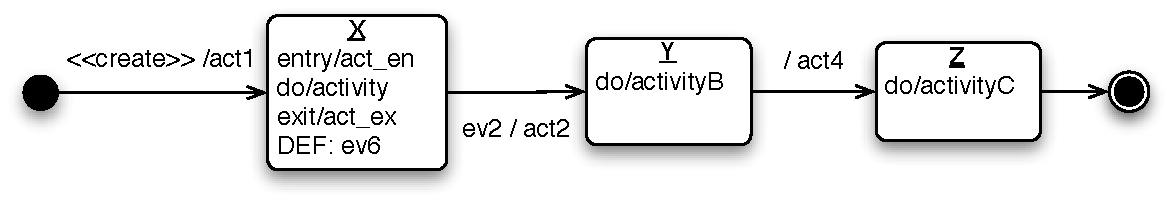
\includegraphics[scale=0.75]{SM.pdf}
	\end{center}
	\caption{Ejemplo de M�quina de Estados.}
	\label{fig:sm}
\end{figure}

\subsection{Diagrama de colaboraci�n}
\label{subsec:colaboracion}
Un {\bf diagrama de colaboraci�n} es un diagrama de interacci�n que destaca la organizaci�n estructural de los objetos que se comunican entre s�. Los diagramas de interacci�n muestran las relaciones existentes entre un grupo de objetos, incluyendo los mensajes que se pueden enviar entre ellos.

\begin{figure}[H]
	\begin{center}
		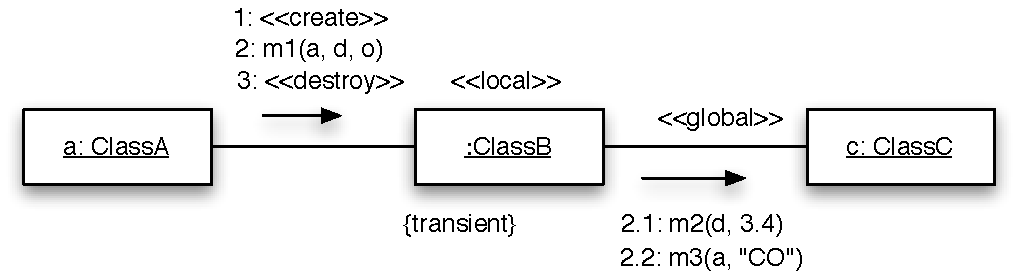
\includegraphics[scale=0.75]{collaboration.pdf}
	\end{center}
	\caption{Ejemplo de Diagrama de Colaboraci�n.}
	\label{fig:collaboration}
\end{figure}

Uno de los elementos m�s importantes dentro del diagrama de colaboraci�n ser� el {\em n�mero de secuencia}, �ste indicar� la ordenaci�n temporal del mensaje, este n�mero se forma con un d�gito que se ir� incrementando secuencialmente por cada nuevo mensaje en el flujo de control. Para soportar el anidamiento, se utiliza la {\em numeraci�n decimal de Dewey} \cite{DDC} en la que, el 1 representa al primer mensaje, el 1.1 ser� el primer mensaje dentro del mensaje 1, el 1.2 ser� el segundo mensaje dentro del mensaje 1, soportando cualquier nivel de profundidad.

%Buscar informaci�n sobre Dewey para la presentaci�n del pfc

Por �ltimo decir que los diagramas de colaboraci�n y los diagramas de secuencia son sem�nticamente equivalentes, debido a que derivan de la misma informaci�n del metamodelo de UML, lo cual hace que presenten unas capacidades similares de expresividad.

\subsection{Mecanismos de extensi�n}
\label{subsec:extension}
Estos mecanismos son proporcionados para posibilitar la expresi�n de todos los matices posibles de todos los modelos en cualquier dominio, en nuestro caso en el dominio de las prestaciones. Los mecanismos con los que contamos en este lenguaje son:

\begin{itemize}
\item {\bf Estereotipos}: permite la creaci�n de nuevos bloques de construcci�n que deriven de los existentes pero que sean espec�ficos del sistema.
\item {\bf Valores etiquetados}: extiende las propiedades de un bloque de construcci�n de UML, para a�adir nueva informaci�n en la especificaci�n de ese elemento.
\item {\bf Restricciones}: extiende la sem�ntica de un bloque de construcci�n.
\end{itemize}

Los elementos que utilizaremos para ser capaces de anotar los modelos de UML con caracter�sticas de prestaciones ser�n los estereotipos y los valores etiquetados.

\section{UML-SPT}
Desde su nacimiento UML ha sido utilizado en el desarrollo de multitud de sistemas con restricciones como tiempo, recursos, prestaciones, o seguridad. Con el paso del tiempo se comprob� que este lenguaje carec�a de la expresividad suficiente como para poder modelar estas caracter�sticas, lo cual limitaba su expansi�n a campos como sistemas de tiempo real o sistemas empotrados.

A pesar de esto se vio que era posible utilizar los mecanismos de extensi�n (ver \ref{subsec:extension}) que facilita con el fin de introducir este tipo de caracter�sticas dentro de nuestros modelos.

El OMG elabor� un documento denominado, {\bf UML} Profile for {\bf S}chedulability, {\bf P}erformance and {\bf T}ime Specification ({\bf UML-SPT}) \cite{UML-SPT}, en el cual se recogen los m�todos com�nes para enriquecer un modelo de UML con informaci�n para su posterior an�lisis de prestaciones. Estos m�todos son los que ha seguido ArgoSPE en su implementaci�n.

La organizaci�n de este documento sigue un esquema l�gico, cada cap�tulo nos instruye en un dominio concreto, por ejemplo el modelado general del tiempo, o el de la concurrencia. Todos los cap�tulos constan de dos partes, la primera introduce los conceptos te�ricos del dominio al que nos estamos referiendo y la segunda explica como modelarlos con los elementos que nos proporciona UML, esta estructura queda reflejada en el siguiente esquema:

%\begin{figure}[hbt]
\begin{figure}[H]
	\begin{center}
		%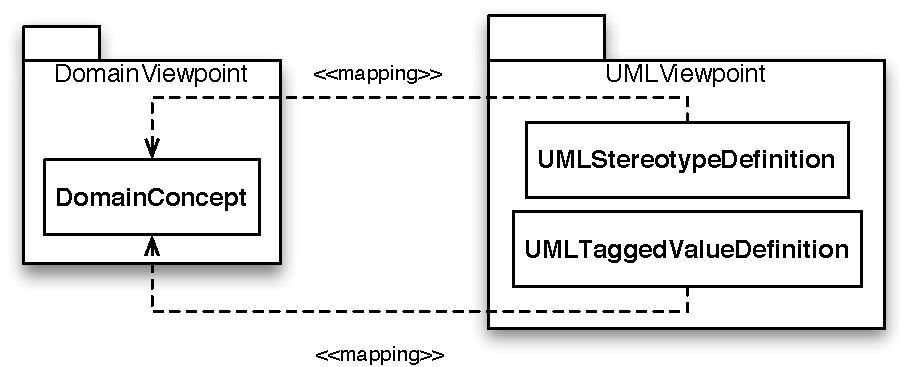
\includegraphics[height=2cm]{UML-SPT.pdf}
		%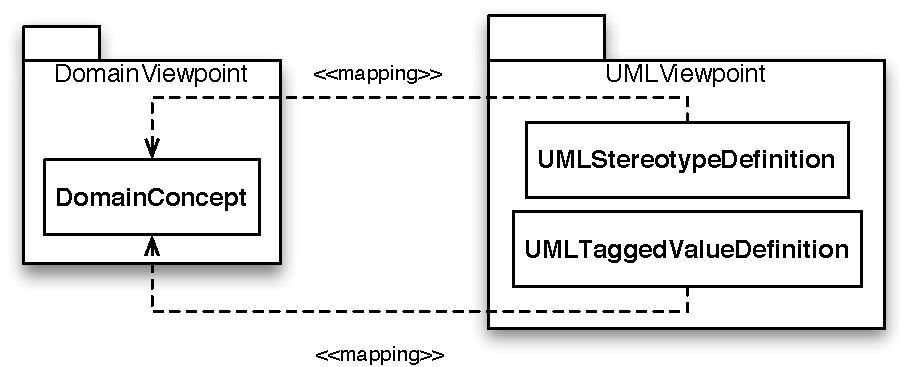
\includegraphics[width=\textwidth]{UML-SPT.pdf}
		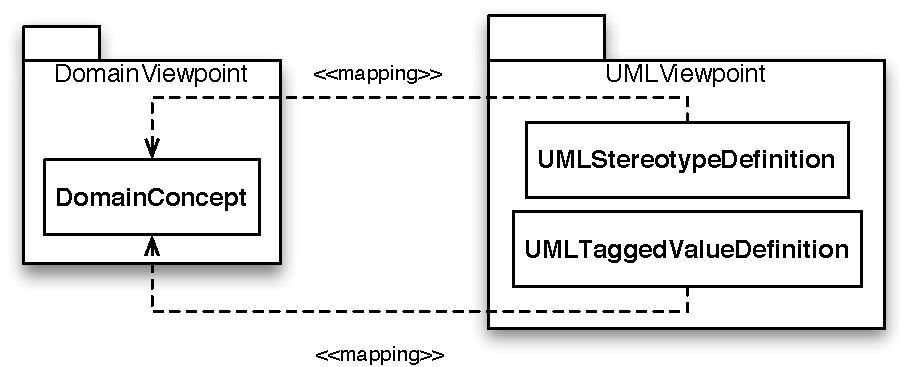
\includegraphics[scale=0.75]{UML-SPT.pdf}
	\end{center}
	\caption{Relaciones entre el punto de vista del dominio y el de UML.}
	\label{fig:UML-SPT}
\end{figure}

La figura \ref{fig:UML-SPT} ilustra uno de estos conceptos del dominio en cuesti�n, el cual ser� representado por un par, estereotipo-valor etiquetado en UML. Los t�rminos m�s interesantes desde el punto de vista del modelado de prestaciones seg�n el UML-SPT son los siguientes:

\begin{itemize}
\item {\bf Contexto}: representa una situaci�n relevante para el dise�ador, dentro de nuestro sistema. Est� constitu�do por varios escenarios.
\item {\bf Escenario}: es una secuencia de 1 o m�s pasos, los cuales est�n ordenados de forma que podremos establecer relaciones de predecesores y sucesores entre los mismos.
Se utilizan para explorar varias situaciones din�micas que envuelven a un conjunto de recursos.
\item {\bf Paso}: incremento en la ejecuci�n de un escenario particular utilizando ciertos recursos.
\item {\bf Recurso}: es visto como un servidor que posee un tiempo de servicio, podemos ver a los pasos como clientes de estos servidores.
\item {\bf Carga de trabajo}: indica la intensidad de la demanda para la ejecuci�n de un escenario espec�fico. Existen dos tipos: las {\em abiertas} que modelan un flujo de peticiones, y las {\em cerradas} que caracterizan un n�mero constante de usuarios.
\end{itemize}

Dentro de la evaluaci�n de prestaciones los escenarios juegan un papel importante puesto que las prestaciones son propiedades din�micas de los  sistemas, para modelarlos utilizando UML tendremos que utilizar alg�n elemento que represente tambi�n propiedades din�micas, en nuestro caso, los {\bf diagramas de colaboraci�n} (ver \ref{subsec:colaboracion}). La representaci�n concreta de los conceptos mencionados con anterioridad quedar� expuesta en el anexo \ref{chap:case}.

\section{Redes de Petri}

En la investigaci�n previa a mi trabajo se decantaron por las redes de Petri como formalismo para la evaluaci�n de prestaciones. Despu�s de una comparativa entre diferentes formalismos como por ejemplo las redes de colas \cite{MolloyBook} o las �lgebras de procesos \cite{HR-98}, se lleg� a la conclusi�n de que las redes de Petri proporcionaban un nivel de detalle mayor para modelar los sistemas que cualquiera de las anteriores. Ahora vamos a proceder a una breve explicaci�n.

Las redes de Petri \cite{Silva-85} ({\bf RdP}) son una herramienta gr�fica para la descripci�n formal de sistemas cuyos comportamientos din�micos est�n caracterizados por la concurrencia, sincronizaci�n, exclusi�n mutua y conflictos. 

La RdP est� representada por un grafo dirigido bipartito en el cual los lugares se representan como c�rculos y las transiciones son dibujadas como barras o como cajas. Los lugares suelen describir estados locales del sistema, mientras que las transiciones representar�an los eventos que modifican el estado del sistema.

El comportamiento din�mico de las RdP est� dirigido por la {\em regla de disparo}, una transici�n puede dispararse si todos sus {\em lugares de entrada} contienen al menos una marca, entonces decimos que la transici�n est� sensibilizada, tras dispararse la transici�n eliminamos una marca de cada uno de los lugares de entrada y generamos una marca en sus {\em lugares de salida}.

Una de las evoluciones que se han producido de las RdP es la introducci�n del concepto del tiempo, por ejemplo a trav�s de transiciones con tiempo, es decir, que ahora tenemos dos tipos de transiciones las inmediatas y las temporizadas. Una RdP con estas caracter�sticas la denominaremos estoc�stica o {\bf SPN}.

Al introducir transiciones con tiempo tambi�n ser� necesario a�adir prioridades a las transiciones, esto evita situaciones conflictivas dentro de la red \cite{GSPN-book}, aqu� s�lo comentaremos que las prioridades ser�n n�meros naturales asociados a las transiciones y que la transici�n con mayor prioridad se disparar� primero si hay posibilidad de que otra tambi�n se pueda disparar.

Las {\bf GSPN}'s ser�n SPN's (con prioridades) en las cuales las transiciones con tiempo tienen definido el retraso de su disparo como una variable aleatoria exponencialmente distribu�da.

\subsection{Operador composici�n}
Para realizar la traducci�n autom�tica de UML a GSPN's ser� necesario un operador que una varias GSPN's en una �nica red, para ello necesitaremos a�adir etiquetas tanto a las transiciones como a los lugares de cada una de las redes que queremos fusionar, este nuevo tipo de redes las llamaremos GSPN etiquetadas o bien {\bf LGSPN}'s.

El resultado de componer lugares y transiciones de dos LGSPN's ser� algo como lo siguiente:

\begin{figure}[H]
	\begin{center}
		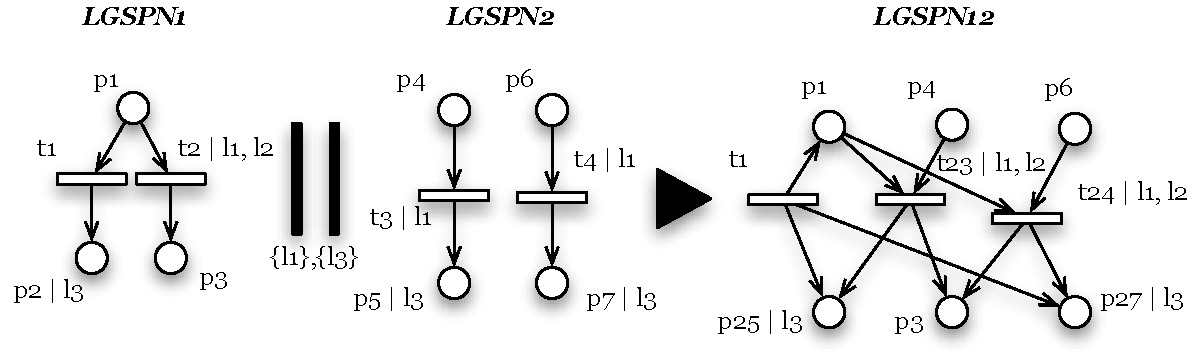
\includegraphics[scale=0.7]{compose.pdf}
	\end{center}
	\caption{Funcionamiento del operador composici�n.}
	\label{fig:compose}
\end{figure}

%En la figura anterior es preciso comentar que los lugares de la red han sido etiquetados con {\em px}, %las transiciones est�n denotadas como {\em tx}, las etiquetas ({\bf �tiles para la composici�n}) ser�n %{\em lx}, y hemos utilizado una {\em tuber�a} como delimitador entre el nombre y las etiquetas.

A continuaci�n vamos a explicar con un poco m�s en detalle una de las etiquetas que forman parte de la figura \ref{fig:compose},  en concreto, \verb!t2|l1,l2!, �sta consta de varias partes, la primera constituye el nombre de la transici�n,  \verb!t2! en este caso, lo siguiente es el separador, \verb! | !, y tras �ste nos encontraremos con una secuencia de etiquetas que utilizaremos para la {\bf composici�n}, \verb!l1! y \verb!l2!.

\section{ArgoSPE}

ArgoSPE es una herramienta fruto de varios proyectos fin de carrera, que ya han sido comentados con anterioridad, adem�s de varias becas de colaboraci�n. Ha sido desarrollada bajo la licencia p�blica de GNU \cite{GNU} (anexo \ref{chap:gpl}).

Esta aplicaci�n tiene como fin poder evaluar las prestaciones de un sistema modelado con ArgoUML (por ahora\footnote{Futuras implementaciones de nuestro m�dulo podr�n utilizar cualquier herramienta CASE (Computer Assisted Software Engineering) como Editor del Modelo, dado que lo permite esta arquitectura flexible.}), implementa muchas de las caracter�sticas ofrecidas en los trabajos \cite{BCDM-TSE,LGMC-WOSP04,MBCD-WODES02} y sigue la arquitectura sugerida en el UML-SPT, representada en la figura \ref{fig:arquitectura}.
%ver figura \ref{fig:arquitectura}.

\begin{figure}[H]
	\begin{center}
		%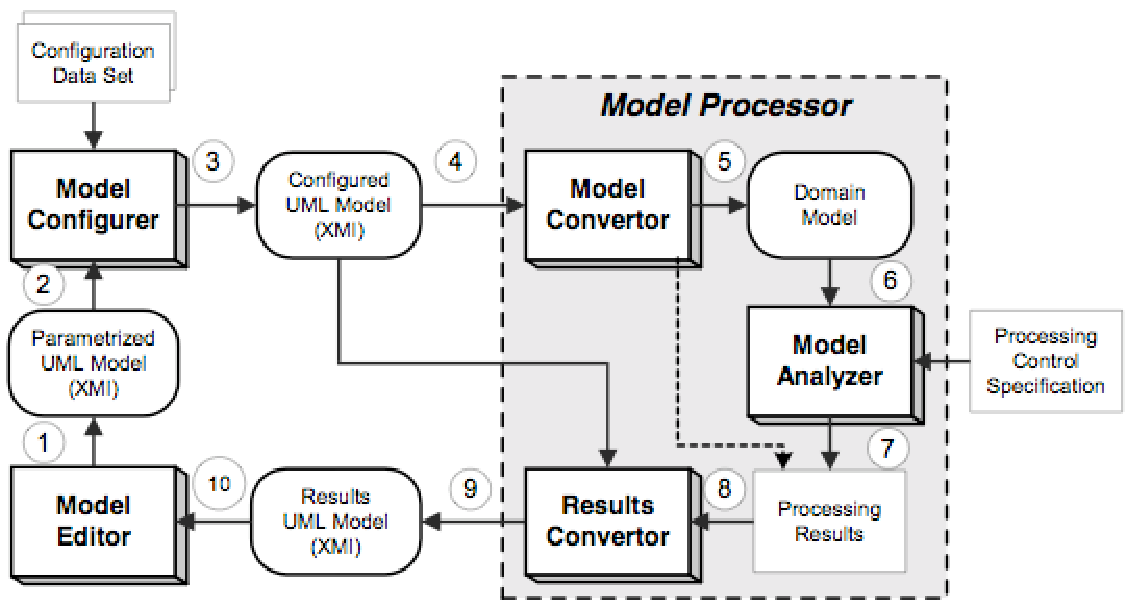
\includegraphics[scale=0.7]{arquitectura.pdf}
		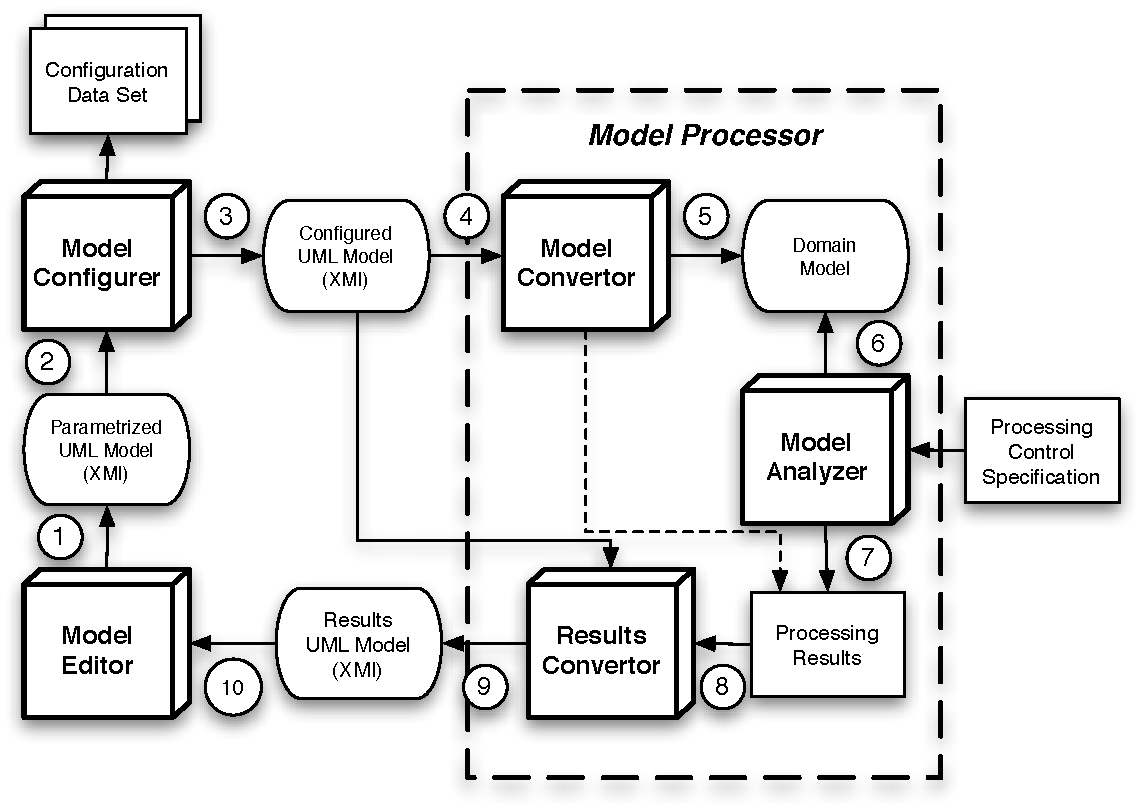
\includegraphics[scale=0.6]{arquitecture.pdf}
	\end{center}
	\caption{Arquitectura sugerida por el UML-SPT.}
	\label{fig:arquitectura}
\end{figure}

Para finalizar comentar que est� dise�ada como un conjunto de paquetes de Java  y es implementada como un plug-in (o m�dulo) de ArgoUML,  para la versi�n {\bf 0.18.1}.

Como queda reflejado en la figura \ref{fig:arquitectura} las principales partes de la arquitectura son el {\bf editor}, el {\bf configurador} y el {\bf procesador del modelo}, este �ltimo est� dividido en {\bf conversor} y {\bf analizador del modelo} y en el {\bf conversor de resultados}.

Esta separaci�n funcional de la arquitectura provoca que se pueda utilizar cualquier herramienta para que aporte la funcionalidad concreta, por ejemplo, se podr�an utilizar diversos programas como analizadores del modelo, aunque para ello deber�amos tener que representar el modelo a analizar en un formato est�ndar y comprensible por dichas herramientas. 

Incluso podr�amos considerar el cambio de formalismo utilizado para el an�lisis, lo que da idea de la potencia de la arquitectura de ArgoSPE.

En la siguiente figura podemos observar c�mo, la estructura de paquetes que constituyen parte de los fuentes de nuestro m�dulo, representa la arquitectura propuesta en el UML-SPT.

\begin{figure}[H]
	\begin{center}
		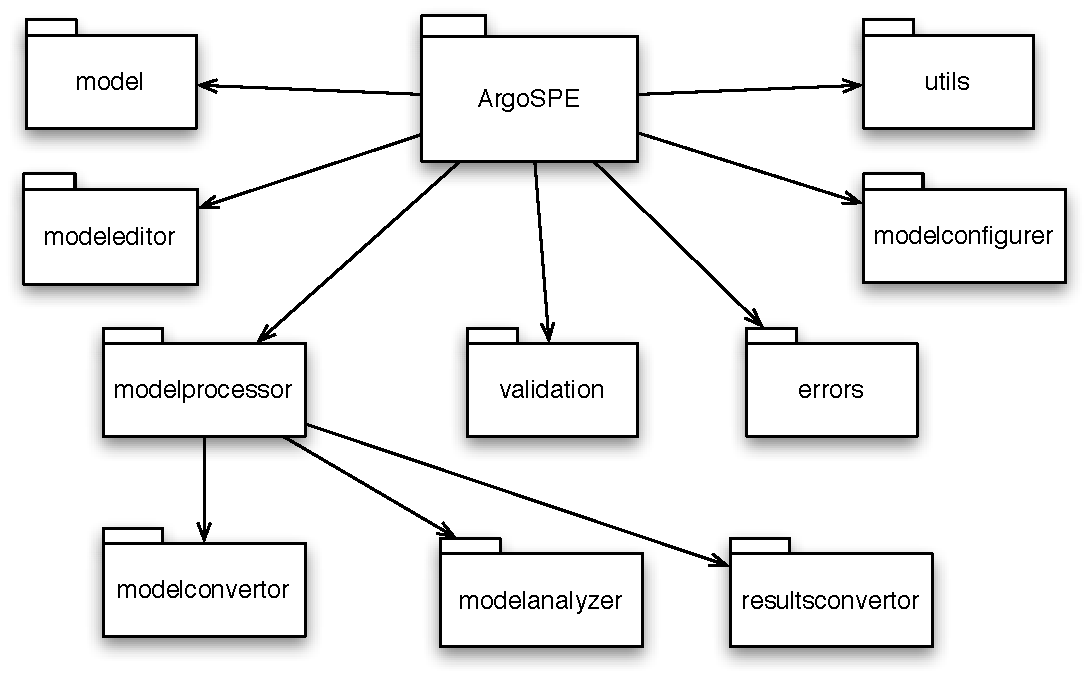
\includegraphics[scale=0.7]{packages.pdf}
	\end{center}
	\caption{Distribuci�n en paquetes de la arquitectura de ArgoSPE.}
	\label{fig:paquetes}
\end{figure}

Las funcionalidades de los principales componentes que conforman la arquitectura son \cite{QEST05-GMM}: 

\begin{itemize}
\item {\bf Editor del Modelo}: este m�dulo debe ofrecer la posibilidad de crear, editar y anotar, usando el {\bf T}agged {\bf V}alue {\bf L}anguage ({\bf TVL} o Lenguaje de Valores Etiquetados), modelos software en UML.
\item {\bf Configurador del Modelo}: su funcionalidad consiste en sustituir los valores etiquetados que poseen expresiones en TVL, por el resultado de evaluar las expresiones, gracias a un fichero de configuraci�n. Pasando a tener un modelo con el XMI configurado.
\item El {\bf Procesador del Modelo} como vemos en la figura \ref{fig:paquetes} est� dividido en:
	\begin{itemize}
		\item {\bf Conversor del Modelo}: es la parte encargada de pasar de un modelo en formato XMI al mismo modelo representado con GSPN's.
		\item {\bf Analizador del Modelo}: este componente ejecuta las consultas realizadas por el usuario utilizando para ello la aplicaci�n GreatSPN.
		\item {\bf Conversor de resultados}: su objetivo es hacer regresar los valores obtenidos por el analizador, al editor del modelo, para que puedan ser recibidos por el usuario.
	\end{itemize}
\end{itemize}
	%\chapter{Conceptos Previos}
\label{chap:concepts}
En el cap�tulo que nos ocupa vamos a poner de manifiesto algunos de los aspectos m�s relevantes dentro de cada una de las �reas que han sido objetivo de mi proyecto fin de carrera.

El objetivo del presente cap�tulo es poner en contexto al lector en las diferentes teor�as y herramientas utilizadas en nuestro trabajo con el fin de que se pueda entender el resto de los cap�tulos. Obviamente estas peque�as introducciones a cada una de las teor�as no ponen de manifiesto la profundidad que el proyectando ha adquirido en cada una de ellas.
 
\section{Estado del Arte}
Hoy en d�a el n�mero de usuarios de herramientas inform�ticas ha crecido enormemente con respecto a �pocas pasadas, este fen�meno es debido fundamentalmente al gran auge de Internet, que ha abierto las puertas de la inform�tica a un cuantioso colectivo de personas. 

Por otro lado las empresas que desarrollan software sacan al mercado aplicaciones cada vez m�s complejas, con un n�mero mayor de funcionalidades que intentan mejorar las ya existentes, y las cuales se desarrollan a una velocidad vertiginosa.

La alta exigencia de calidad, robustez, eficiencia y funcionalidad por parte de todos esos usuarios que hemos comentado, hace que la industria del software tenga que recurrir a disciplinas que ayuden a conseguir todos estos prop�sitos. 

Este es el caso de la {\bf Ingenier�a del software} \cite{Pressman} que se encarga de optimizar el proceso de desarrollo de un producto software, con el fin de hacer cumplir los requisitos impuestos evitando pr�cticas que puedan retrasar la finalizaci�n del producto.

El problema existente es que esta disciplina no est� enfocada a asegurar las caracter�sticas del software relacionadas con su rendimiento, lo que obliga cont�nuamente a valorar las prestaciones de un sistema en sus fases finales de desarrollo, con una versi�n funcional.

Esta pr�ctica conlleva riesgos inevitables, por ejemplo, podr�a darse el caso de que una vez conseguida un versi�n funcional, y tras realizar una serie de pruebas llegaramos a la conclusi�n de que no podemos alcanzar los niveles de prestaciones esperados, con lo que habr�amos desaprovechado una gran cantidad de tiempo que no podr�amos recuperar.

Una soluci�n diferente ser�a el adelantar el an�lisis del rendimiento de este tipo de productos a las etapas iniciales de sus ciclos de vida, con el consiguiente ahorro del tiempo invertido en desarrollar un producto, que no va a cumplir con las prestaciones requeridas. Este concepto es la piedra angular de un campo de investigaci�n conocido como {\bf Ingenier�a de Prestaciones del Software} o {\bf SPE} \cite{Connie90}.

En este punto aparece el problema de c�mo incluir este nuevo enfoque al proceso de desarrollo del software actual. UML es, hoy en d�a, el est�ndar de facto en la ingenier�a del software y es utilizado por la gran mayor�a de personas dedicadas al mundo del desarrollo, lo cual lo convierte en el candidato id�neo para incluirle las prestaciones de los sistemas. 

�sta es a grandes rasgos la idea que han seguido los trabajos de investigaci�n realizados en el GISED comentados anteriormente, y que mencionaremos m�s adelante.

Todav�a quedan en el aire preguntas importantes como por ejemplo, �{\bf c�mo} incluiremos las medidas de prestaciones en UML?, �{\bf qu� modelo} utilizaremos para analizar las {\bf prestaciones} que nos van a interesar?, todas estas cuestiones quedar�n respondidas en las secciones siguientes.

\section{UML}
%Se puede eliminar y reescribir lo siguiente
El  Object  Management  Group  ({\bf OMG}) \cite{OMG-org}  es  un consorcio a  nivel  internacional  que  integra a los principales representantes de la industria de la tecnolog�a de informaci�n Orientada a Objetos ({\bf OO}). El OMG tiene como objetivo central la promoci�n, y el impulso de la industria OO. �ste propone y adopta por consenso especificaciones en torno a la tecnolog�a OO, especificaciones que se convierten en est�ndar {\bf ISO} por defecto. 

Una de las especificaciones m�s importantes es la adopci�n en 1998 de UML como un est�ndar.  �ste se integra dentro de Model Driven Architecture ({\bf MDA}) de OMG, que es a la  postre un conjunto de est�ndares que sirven para planificar y controlar el ciclo completo  de vida del software, independientemente de la plataforma para la que se desarrolla ese  software. Y es aqu� donde queda clara su relaci�n con lo que conocemos como Ingenier�a  del Software.
 
UML es pues una especificaci�n semi-formal que define un lenguaje gr�fico que nos sirve para  visualizar,  especificar,  construir  y  documentar  los  artefactos  o  elementos  de  nuestro  sistema.
En �l tambi�n se definen reglas sem�nticas y de correcci�n de modelos lo que lo convierten en algo m�s que un lenguaje gr�fico.

UML define {\bf doce} tipos distintos de diagramas gr�ficos, que sirven para  describir todas las vistas que un modelo pueda necesitar para ser caracterizado, vistas que se  ajusten al paradigma OO.  

Estos doce diagramas se agrupan a su vez en tres categor�as: la que incluye diagramas  que  definen  estructuras  o  elementos  est�ticos,  la  compuesta por diagramas  que  definen  diferentes aspectos del comportamiento din�mico y la que engloba diagramas que definen  como organizar los m�dulos de una aplicaci�n. �stas son las tres categor�as respectivas, junto con los nombres de los diagramas que forman parte de ellas: 

\begin{itemize}
\item {\bf Diagramas  estructurales}:  diagrama  de  clases,  diagrama  de  objetos,  diagrama de componentes y diagrama de despliegue.
\item {\bf Diagramas de comportamiento}: diagrama de casos de uso, diagrama de  secuencia, diagrama de actividad, diagrama de colaboraci�n y diagrama (o m�quinas) de estados.
\item {\bf Diagramas  de  organizaci�n  del  modelo}:  diagramas  de  paquetes,  subsistemas y de modelos.  
\end{itemize}

Es momento de realizar una breve presentaci�n de los dos tipos de diagramas que participan m�s activamente en mi proyecto: M�quina de Estados y Diagrama de Colaboraci�n.

\subsection{M�quina de estados}
Una {\bf m�quina de estados} se utiliza para modelar los aspectos din�micos de un sistema. La mayor�a de las veces esto supone el modelado del comportamiento de objetos  que reaccionan ante los eventos lanzados desde fuera de su contexto.

Los estados son los elementos primordiales de este tipo de diagramas. Un estado es  una  condici�n  o  situaci�n  en  la  vida  de  un  objeto  durante  la  cual  satisface  alguna  condici�n, realiza alguna actividad o espera alg�n evento. En esta figura se muestra un diagrama de estados gen�rico:

\begin{figure}[H]
	\begin{center}
		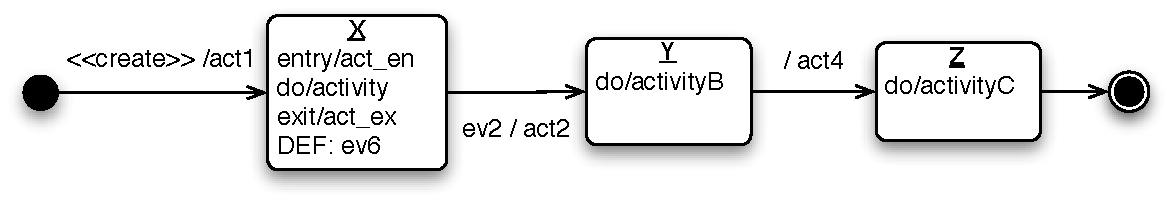
\includegraphics[scale=0.75]{SM.pdf}
	\end{center}
	\caption{Ejemplo de M�quina de Estados.}
	\label{fig:sm}
\end{figure}

\subsection{Diagrama de colaboraci�n}
\label{subsec:colaboracion}
Un {\bf diagrama de colaboraci�n} es un diagrama de interacci�n que destaca la organizaci�n estructural de los objetos que se comunican entre s�. Los diagramas de interacci�n muestran las relaciones existentes entre un grupo de objetos, incluyendo los mensajes que se pueden enviar entre ellos.

\begin{figure}[H]
	\begin{center}
		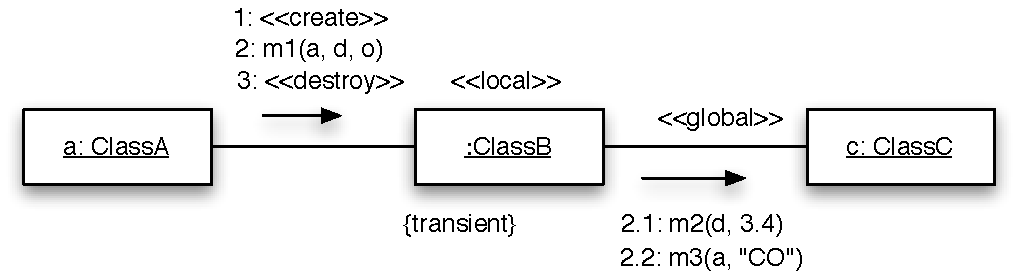
\includegraphics[scale=0.75]{collaboration.pdf}
	\end{center}
	\caption{Ejemplo de Diagrama de Colaboraci�n.}
	\label{fig:collaboration}
\end{figure}

Uno de los elementos m�s importantes dentro del diagrama de colaboraci�n ser� el {\em n�mero de secuencia}, �ste indicar� la ordenaci�n temporal del mensaje, este n�mero se forma con un d�gito que se ir� incrementando secuencialmente por cada nuevo mensaje en el flujo de control. Para soportar el anidamiento, se utiliza la {\em numeraci�n decimal de Dewey} \cite{DDC} en la que, el 1 representa al primer mensaje, el 1.1 ser� el primer mensaje dentro del mensaje 1, el 1.2 ser� el segundo mensaje dentro del mensaje 1, soportando cualquier nivel de profundidad.

%Buscar informaci�n sobre Dewey para la presentaci�n del pfc

Por �ltimo decir que los diagramas de colaboraci�n y los diagramas de secuencia son sem�nticamente equivalentes, debido a que derivan de la misma informaci�n del metamodelo de UML, lo cual hace que presenten unas capacidades similares de expresividad.

\subsection{Mecanismos de extensi�n}
\label{subsec:extension}
Estos mecanismos son proporcionados para posibilitar la expresi�n de todos los matices posibles de todos los modelos en cualquier dominio, en nuestro caso en el dominio de las prestaciones. Los mecanismos con los que contamos en este lenguaje son:

\begin{itemize}
\item {\bf Estereotipos}: permite la creaci�n de nuevos bloques de construcci�n que deriven de los existentes pero que sean espec�ficos del sistema.
\item {\bf Valores etiquetados}: extiende las propiedades de un bloque de construcci�n de UML, para a�adir nueva informaci�n en la especificaci�n de ese elemento.
\item {\bf Restricciones}: extiende la sem�ntica de un bloque de construcci�n.
\end{itemize}

Los elementos que utilizaremos para ser capaces de anotar los modelos de UML con caracter�sticas de prestaciones ser�n los estereotipos y los valores etiquetados.

\section{UML-SPT}
Desde su nacimiento UML ha sido utilizado en el desarrollo de multitud de sistemas con restricciones como tiempo, recursos, prestaciones, o seguridad. Con el paso del tiempo se comprob� que este lenguaje carec�a de la expresividad suficiente como para poder modelar estas caracter�sticas, lo cual limitaba su expansi�n a campos como sistemas de tiempo real o sistemas empotrados.

A pesar de esto se vio que era posible utilizar los mecanismos de extensi�n (ver \ref{subsec:extension}) que facilita con el fin de introducir este tipo de caracter�sticas dentro de nuestros modelos.

El OMG elabor� un documento denominado, {\bf UML} Profile for {\bf S}chedulability, {\bf P}erformance and {\bf T}ime Specification ({\bf UML-SPT}) \cite{UML-SPT}, en el cual se recogen los m�todos com�nes para enriquecer un modelo de UML con informaci�n para su posterior an�lisis de prestaciones. Estos m�todos son los que ha seguido ArgoSPE en su implementaci�n.

La organizaci�n de este documento sigue un esquema l�gico, cada cap�tulo nos instruye en un dominio concreto, por ejemplo el modelado general del tiempo, o el de la concurrencia. Todos los cap�tulos constan de dos partes, la primera introduce los conceptos te�ricos del dominio al que nos estamos referiendo y la segunda explica como modelarlos con los elementos que nos proporciona UML, esta estructura queda reflejada en el siguiente esquema:

%\begin{figure}[hbt]
\begin{figure}[H]
	\begin{center}
		%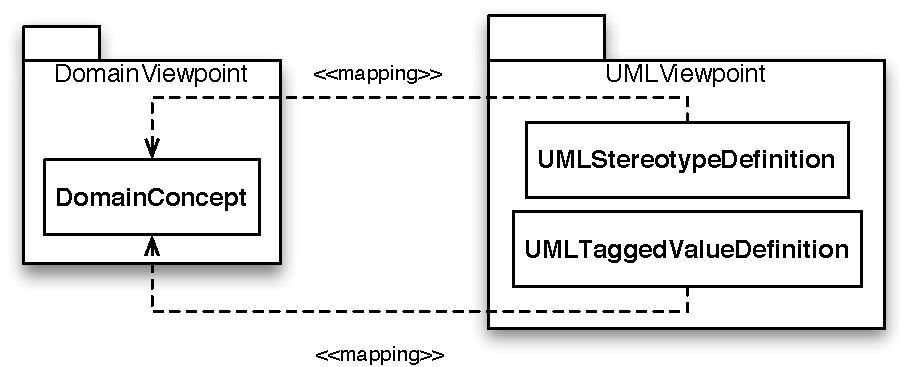
\includegraphics[height=2cm]{UML-SPT.pdf}
		%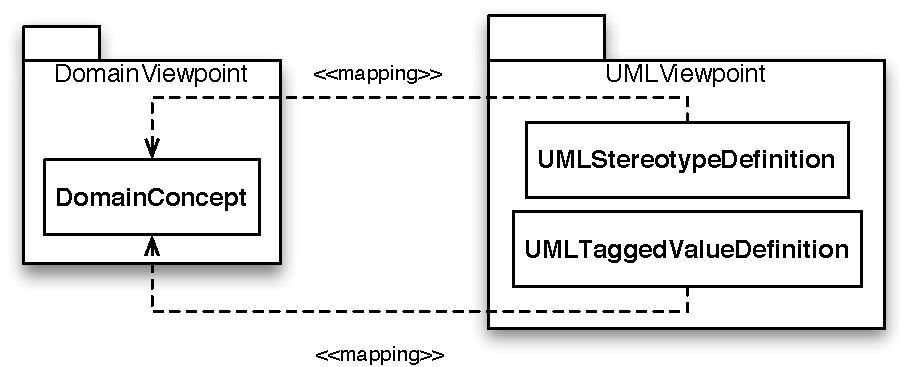
\includegraphics[width=\textwidth]{UML-SPT.pdf}
		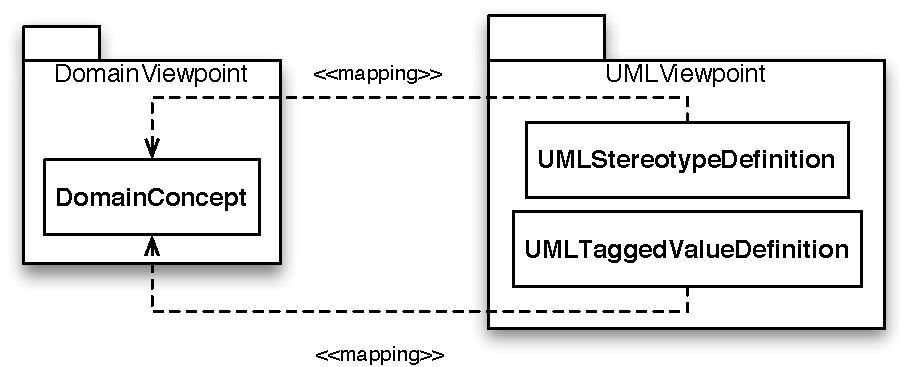
\includegraphics[scale=0.75]{UML-SPT.pdf}
	\end{center}
	\caption{Relaciones entre el punto de vista del dominio y el de UML.}
	\label{fig:UML-SPT}
\end{figure}

La figura \ref{fig:UML-SPT} ilustra uno de estos conceptos del dominio en cuesti�n, el cual ser� representado por un par, estereotipo-valor etiquetado en UML. Los t�rminos m�s interesantes desde el punto de vista del modelado de prestaciones seg�n el UML-SPT son los siguientes:

\begin{itemize}
\item {\bf Contexto}: representa una situaci�n relevante para el dise�ador, dentro de nuestro sistema. Est� constitu�do por varios escenarios.
\item {\bf Escenario}: es una secuencia de 1 o m�s pasos, los cuales est�n ordenados de forma que podremos establecer relaciones de predecesores y sucesores entre los mismos.
Se utilizan para explorar varias situaciones din�micas que envuelven a un conjunto de recursos.
\item {\bf Paso}: incremento en la ejecuci�n de un escenario particular utilizando ciertos recursos.
\item {\bf Recurso}: es visto como un servidor que posee un tiempo de servicio, podemos ver a los pasos como clientes de estos servidores.
\item {\bf Carga de trabajo}: indica la intensidad de la demanda para la ejecuci�n de un escenario espec�fico. Existen dos tipos: las {\em abiertas} que modelan un flujo de peticiones, y las {\em cerradas} que caracterizan un n�mero constante de usuarios.
\end{itemize}

Dentro de la evaluaci�n de prestaciones los escenarios juegan un papel importante puesto que las prestaciones son propiedades din�micas de los  sistemas, para modelarlos utilizando UML tendremos que utilizar alg�n elemento que represente tambi�n propiedades din�micas, en nuestro caso, los {\bf diagramas de colaboraci�n} (ver \ref{subsec:colaboracion}). La representaci�n concreta de los conceptos mencionados con anterioridad quedar� expuesta en el anexo \ref{chap:case}.

\section{Redes de Petri}

En la investigaci�n previa a mi trabajo se decantaron por las redes de Petri como formalismo para la evaluaci�n de prestaciones. Despu�s de una comparativa entre diferentes formalismos como por ejemplo las redes de colas \cite{MolloyBook} o las �lgebras de procesos \cite{HR-98}, se lleg� a la conclusi�n de que las redes de Petri proporcionaban un nivel de detalle mayor para modelar los sistemas que cualquiera de las anteriores. Ahora vamos a proceder a una breve explicaci�n.

Las redes de Petri \cite{Silva-85} ({\bf RdP}) son una herramienta gr�fica para la descripci�n formal de sistemas cuyos comportamientos din�micos est�n caracterizados por la concurrencia, sincronizaci�n, exclusi�n mutua y conflictos. 

La RdP est� representada por un grafo dirigido bipartito en el cual los lugares se representan como c�rculos y las transiciones son dibujadas como barras o como cajas. Los lugares suelen describir estados locales del sistema, mientras que las transiciones representar�an los eventos que modifican el estado del sistema.

El comportamiento din�mico de las RdP est� dirigido por la {\em regla de disparo}, una transici�n puede dispararse si todos sus {\em lugares de entrada} contienen al menos una marca, entonces decimos que la transici�n est� sensibilizada, tras dispararse la transici�n eliminamos una marca de cada uno de los lugares de entrada y generamos una marca en sus {\em lugares de salida}.

Una de las evoluciones que se han producido de las RdP es la introducci�n del concepto del tiempo, por ejemplo a trav�s de transiciones con tiempo, es decir, que ahora tenemos dos tipos de transiciones las inmediatas y las temporizadas. Una RdP con estas caracter�sticas la denominaremos estoc�stica o {\bf SPN}.

Al introducir transiciones con tiempo tambi�n ser� necesario a�adir prioridades a las transiciones, esto evita situaciones conflictivas dentro de la red \cite{GSPN-book}, aqu� s�lo comentaremos que las prioridades ser�n n�meros naturales asociados a las transiciones y que la transici�n con mayor prioridad se disparar� primero si hay posibilidad de que otra tambi�n se pueda disparar.

Las {\bf GSPN}'s ser�n SPN's (con prioridades) en las cuales las transiciones con tiempo tienen definido el retraso de su disparo como una variable aleatoria exponencialmente distribu�da.

\subsection{Operador composici�n}
Para realizar la traducci�n autom�tica de UML a GSPN's ser� necesario un operador que una varias GSPN's en una �nica red, para ello necesitaremos a�adir etiquetas tanto a las transiciones como a los lugares de cada una de las redes que queremos fusionar, este nuevo tipo de redes las llamaremos GSPN etiquetadas o bien {\bf LGSPN}'s.

El resultado de componer lugares y transiciones de dos LGSPN's ser� algo como lo siguiente:

\begin{figure}[H]
	\begin{center}
		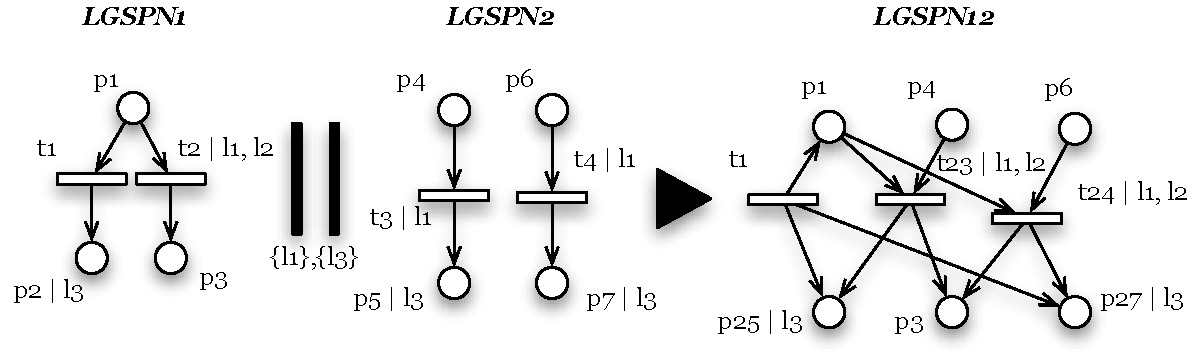
\includegraphics[scale=0.7]{compose.pdf}
	\end{center}
	\caption{Funcionamiento del operador composici�n.}
	\label{fig:compose}
\end{figure}

%En la figura anterior es preciso comentar que los lugares de la red han sido etiquetados con {\em px}, %las transiciones est�n denotadas como {\em tx}, las etiquetas ({\bf �tiles para la composici�n}) ser�n %{\em lx}, y hemos utilizado una {\em tuber�a} como delimitador entre el nombre y las etiquetas.

A continuaci�n vamos a explicar con un poco m�s en detalle una de las etiquetas que forman parte de la figura \ref{fig:compose},  en concreto, \verb!t2|l1,l2!, �sta consta de varias partes, la primera constituye el nombre de la transici�n,  \verb!t2! en este caso, lo siguiente es el separador, \verb! | !, y tras �ste nos encontraremos con una secuencia de etiquetas que utilizaremos para la {\bf composici�n}, \verb!l1! y \verb!l2!.

\section{ArgoSPE}

ArgoSPE es una herramienta fruto de varios proyectos fin de carrera, que ya han sido comentados con anterioridad, adem�s de varias becas de colaboraci�n. Ha sido desarrollada bajo la licencia p�blica de GNU \cite{GNU} (anexo \ref{chap:gpl}).

Esta aplicaci�n tiene como fin poder evaluar las prestaciones de un sistema modelado con ArgoUML (por ahora\footnote{Futuras implementaciones de nuestro m�dulo podr�n utilizar cualquier herramienta CASE (Computer Assisted Software Engineering) como Editor del Modelo, dado que lo permite esta arquitectura flexible.}), implementa muchas de las caracter�sticas ofrecidas en los trabajos \cite{BCDM-TSE,LGMC-WOSP04,MBCD-WODES02} y sigue la arquitectura sugerida en el UML-SPT, representada en la figura \ref{fig:arquitectura}.
%ver figura \ref{fig:arquitectura}.

\begin{figure}[H]
	\begin{center}
		%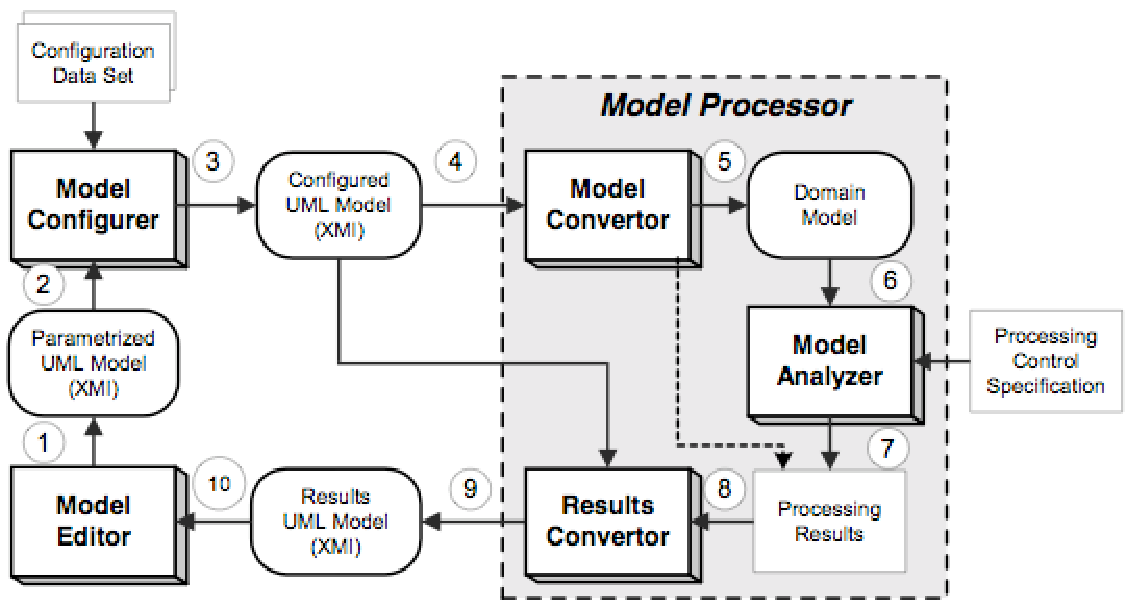
\includegraphics[scale=0.7]{arquitectura.pdf}
		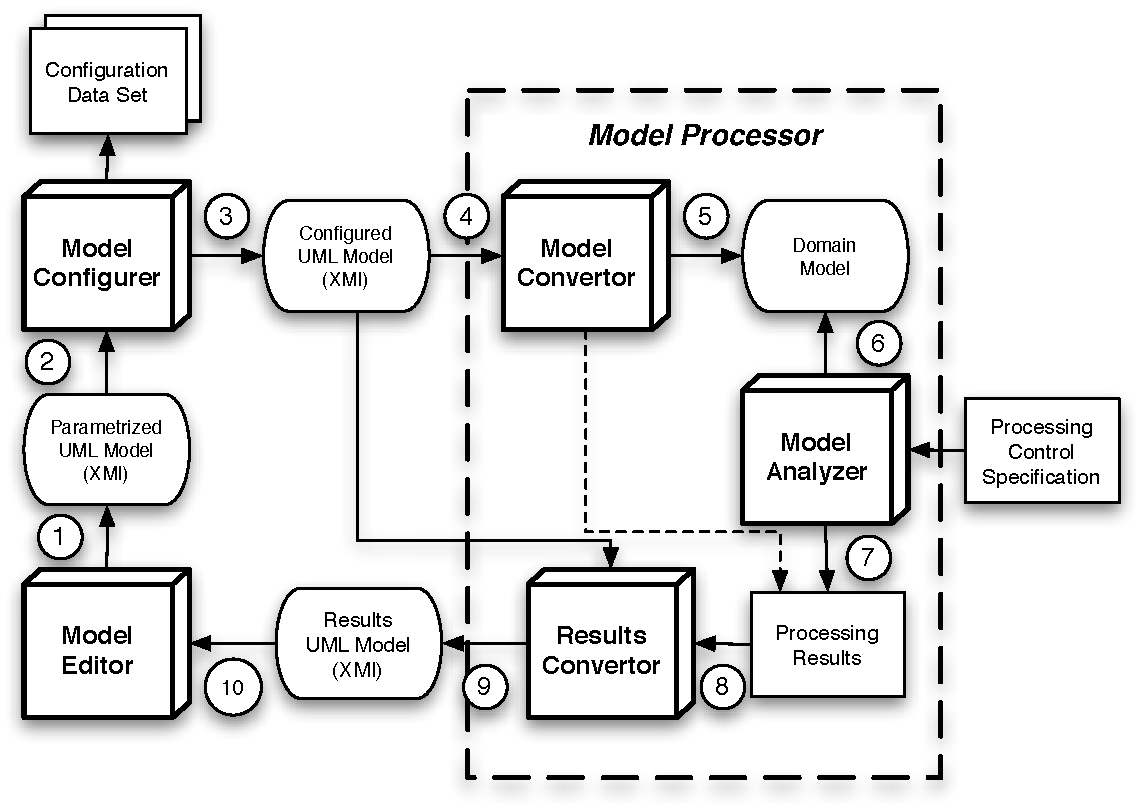
\includegraphics[scale=0.6]{arquitecture.pdf}
	\end{center}
	\caption{Arquitectura sugerida por el UML-SPT.}
	\label{fig:arquitectura}
\end{figure}

Para finalizar comentar que est� dise�ada como un conjunto de paquetes de Java  y es implementada como un plug-in (o m�dulo) de ArgoUML,  para la versi�n {\bf 0.18.1}.

Como queda reflejado en la figura \ref{fig:arquitectura} las principales partes de la arquitectura son el {\bf editor}, el {\bf configurador} y el {\bf procesador del modelo}, este �ltimo est� dividido en {\bf conversor} y {\bf analizador del modelo} y en el {\bf conversor de resultados}.

Esta separaci�n funcional de la arquitectura provoca que se pueda utilizar cualquier herramienta para que aporte la funcionalidad concreta, por ejemplo, se podr�an utilizar diversos programas como analizadores del modelo, aunque para ello deber�amos tener que representar el modelo a analizar en un formato est�ndar y comprensible por dichas herramientas. 

Incluso podr�amos considerar el cambio de formalismo utilizado para el an�lisis, lo que da idea de la potencia de la arquitectura de ArgoSPE.

En la siguiente figura podemos observar c�mo, la estructura de paquetes que constituyen parte de los fuentes de nuestro m�dulo, representa la arquitectura propuesta en el UML-SPT.

\begin{figure}[H]
	\begin{center}
		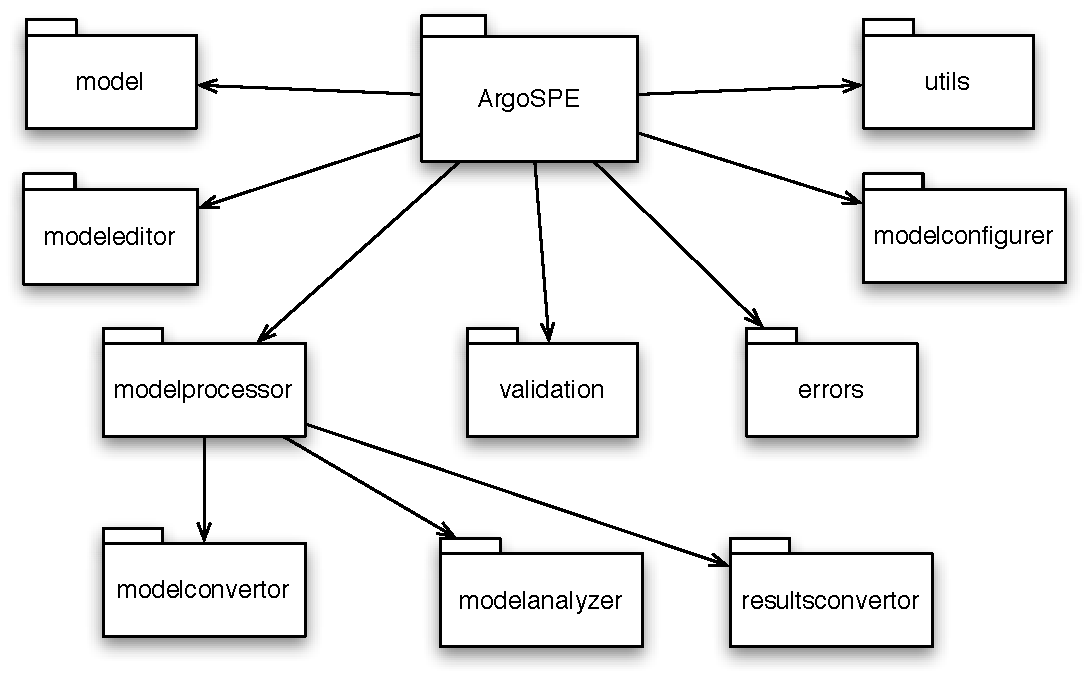
\includegraphics[scale=0.7]{packages.pdf}
	\end{center}
	\caption{Distribuci�n en paquetes de la arquitectura de ArgoSPE.}
	\label{fig:paquetes}
\end{figure}

Las funcionalidades de los principales componentes que conforman la arquitectura son \cite{QEST05-GMM}: 

\begin{itemize}
\item {\bf Editor del Modelo}: este m�dulo debe ofrecer la posibilidad de crear, editar y anotar, usando el {\bf T}agged {\bf V}alue {\bf L}anguage ({\bf TVL} o Lenguaje de Valores Etiquetados), modelos software en UML.
\item {\bf Configurador del Modelo}: su funcionalidad consiste en sustituir los valores etiquetados que poseen expresiones en TVL, por el resultado de evaluar las expresiones, gracias a un fichero de configuraci�n. Pasando a tener un modelo con el XMI configurado.
\item El {\bf Procesador del Modelo} como vemos en la figura \ref{fig:paquetes} est� dividido en:
	\begin{itemize}
		\item {\bf Conversor del Modelo}: es la parte encargada de pasar de un modelo en formato XMI al mismo modelo representado con GSPN's.
		\item {\bf Analizador del Modelo}: este componente ejecuta las consultas realizadas por el usuario utilizando para ello la aplicaci�n GreatSPN.
		\item {\bf Conversor de resultados}: su objetivo es hacer regresar los valores obtenidos por el analizador, al editor del modelo, para que puedan ser recibidos por el usuario.
	\end{itemize}
\end{itemize}
	
	\chapter{Planificaci�n del trabajo} 
\label{chap:schedule}
\section{Diagrama de actividades}
En mi opini�n este proyecto no cuadra con el esquema de un ciclo de vida convencional, esto se debe a que nuestro trabajo consiste en la extensi�n de una herramienta ya existente, como es ArgoSPE. Se ha considerado m�s adecuado describir el modo en que se ha desarrollado mi trabajo gracias a un esquema que tiene mucha similitud con un ciclo de vida en cascada mejorado. La siguiente figura representa el orden cronol�gico de las fases (ver \ref{sec:fases} y \ref{sec:trabajo}) en las se organiz� mi proyecto desde el primer momento.

\begin{figure}[H]
	\begin{center}
		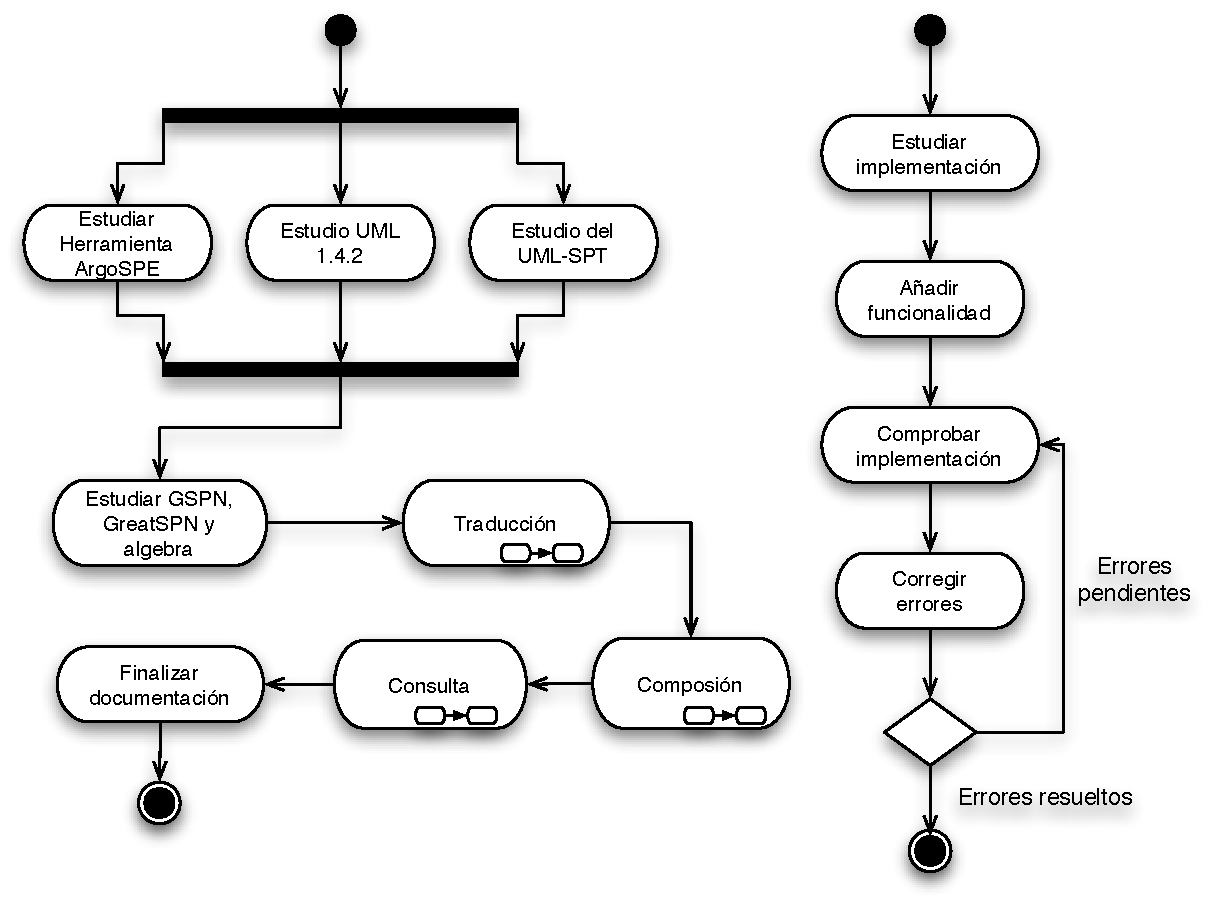
\includegraphics[scale=0.7]{planificacion.pdf}
	\end{center}
	\caption{Diagramas de actividades de la planificaci�n.}
	\label{fig:planificacion}
\end{figure}

\section{Diagrama de Gantt}

\begin{figure}[H]
	\begin{center}
		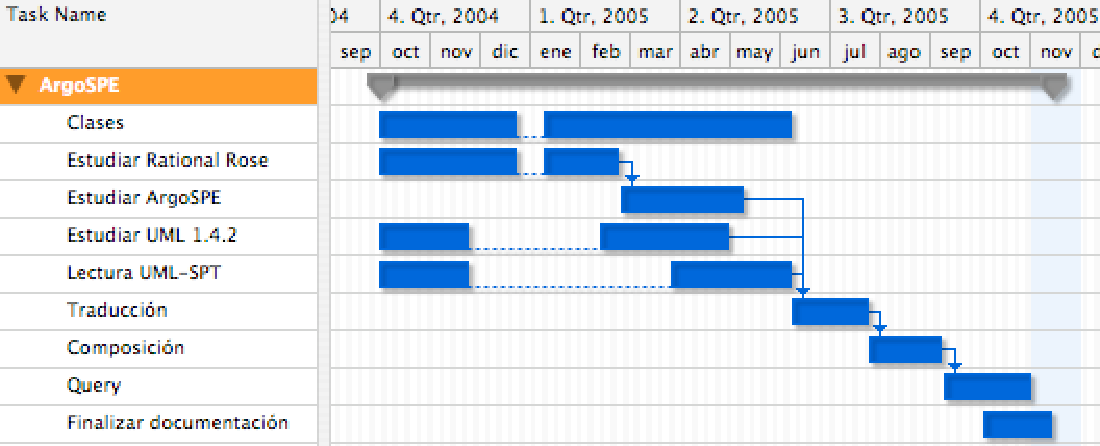
\includegraphics[scale=0.75]{shortgantt.pdf}
	\end{center}
	\caption{Diagrama de la cronolog�a real.}
	\label{fig:gantt}
\end{figure}

En el diagrama anterior queda reflejado (tarea Clases) el hecho de que durante la realizaci�n de este proyecto he tenido que terminar las �ltimas asignaturas de mi carrera,  factor que ha supuesto la prolongaci�n, m�s all� de lo esperado, de algunas tareas relacionadas con mi trabajo.

Otro hecho muy importante que ha marcado el transcurso de mi trabajo fue {\bf estudio de Rational Rose}\footnote{El objetivo original del proyecto era modificar ArgoSPE para que trabajara con Rational Rose.} \cite{Rose}, que consisiti� en la b�squeda y lectura de toda la informaci�n disponible referente a la extensi�n de esta aplicaci�n.

La investigaci�n realizada concluy� con, la implementaci�n de una peque�a extensi�n, en forma de submen�, y con la idea clara de que era {\bf imposible}\footnote{Este t�rmino refleja el hecho de que no disponer de la documentaci�n adecuada prolongar�a en exceso una posible extensi�n, haciendo inviable esa opci�n.} llegar a desarrollar una extensi�n completa, a menos que fu�ramos socios tecnol�gicos de la empresa\footnote{Rational, la empresa desarrolladora, fue adquirida por IBM.} que se dedicaba a la implementaci�n de la herramienta, puesto que la documentaci�n necesaria para ello solamente era distribu�da a estos �ltimos.

El resultado de la investigaci�n hizo que el objetivo de mi proyecto fuera completamente diferente al que en un principio se me hab�a propuesto, a partir de ahora nuestro trabajo iba a consistir en la ampliaci�n de la herramienta ArgoSPE.

A parte de hacer inservible la gran parte del trabajo elaborado en la primera fase, estos cambios produjeron una reestructuraci�n completa de las tareas que se deb�an realizar para conseguir los nuevos objetivos, estas nuevas tareas son las que aparecen en el diagrama anterior a partir de Febrero de 2005.

El gr�fico anterior pone de manifiesto las dependencias existentes entre las tareas en las cuales se ha organizado el trabajo, as� se puede observar que el estudio de la teor�a precede a la implementaci�n de cada una de las partes. Tambi�n observamos que, existe una dependencia entre la traducci�n, la composici�n y la consulta, la cual ha sido respetada.
	%\chapter{Planificaci�n del trabajo} 
\label{chap:schedule}
\section{Diagrama de actividades}
En mi opini�n este proyecto no cuadra con el esquema de un ciclo de vida convencional, esto se debe a que nuestro trabajo consiste en la extensi�n de una herramienta ya existente, como es ArgoSPE. Se ha considerado m�s adecuado describir el modo en que se ha desarrollado mi trabajo gracias a un esquema que tiene mucha similitud con un ciclo de vida en cascada mejorado. La siguiente figura representa el orden cronol�gico de las fases (ver \ref{sec:fases} y \ref{sec:trabajo}) en las se organiz� mi proyecto desde el primer momento.

\begin{figure}[H]
	\begin{center}
		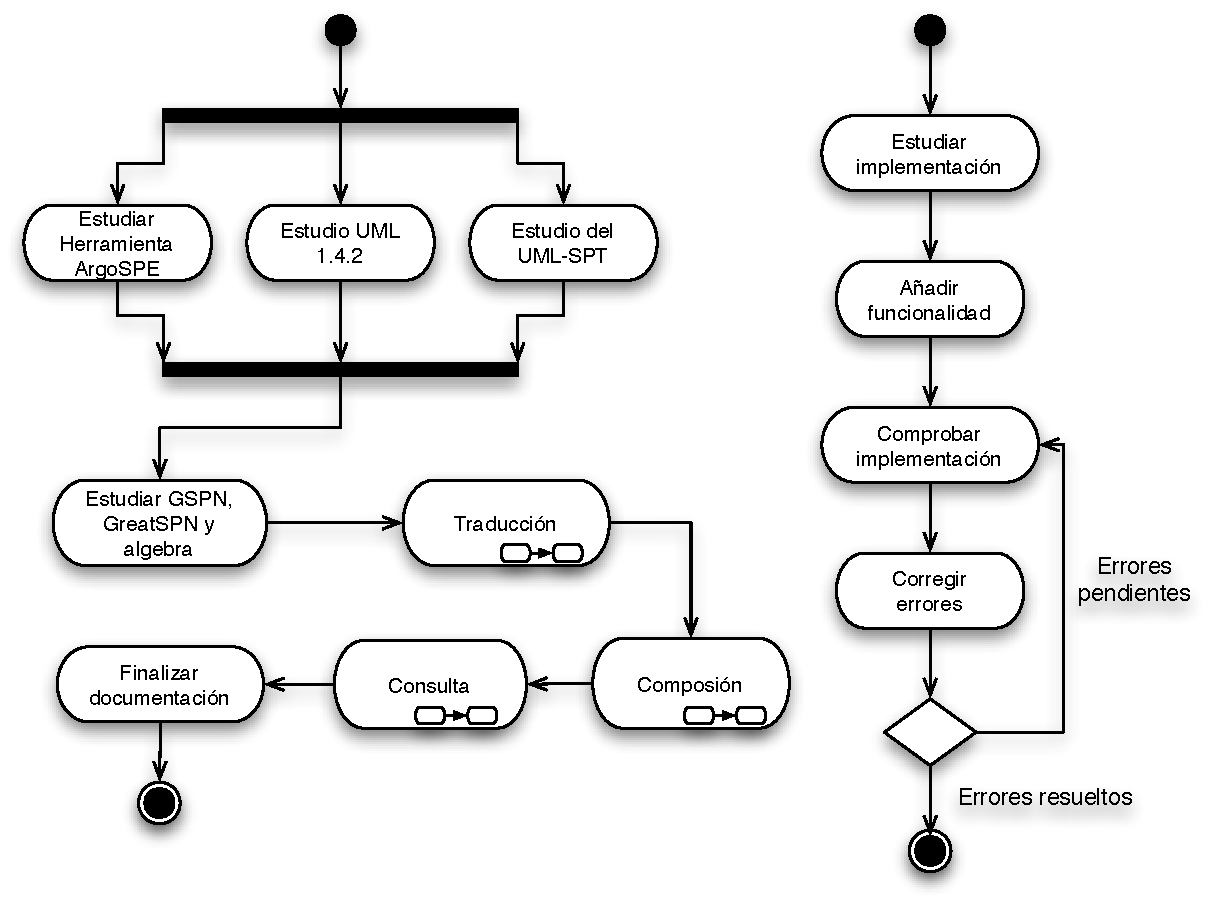
\includegraphics[scale=0.7]{planificacion.pdf}
	\end{center}
	\caption{Diagramas de actividades de la planificaci�n.}
	\label{fig:planificacion}
\end{figure}

\section{Diagrama de Gantt}

\begin{figure}[H]
	\begin{center}
		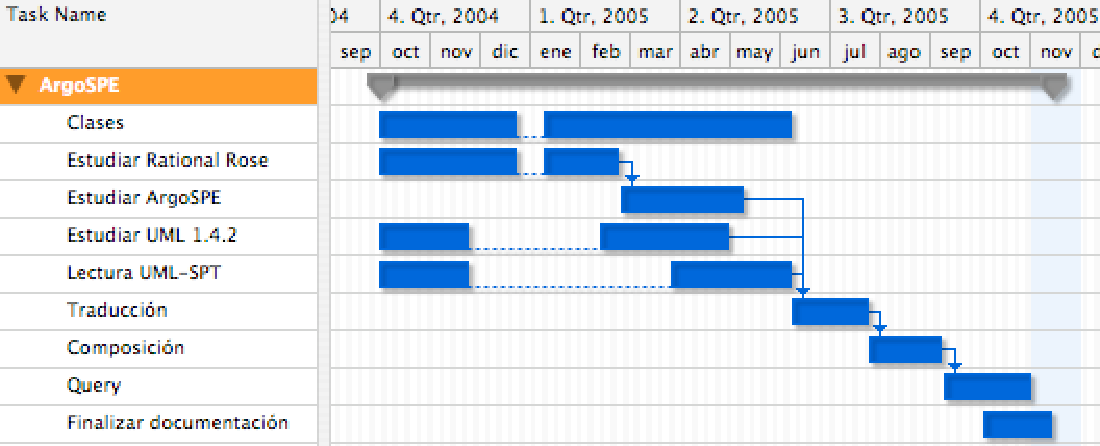
\includegraphics[scale=0.75]{shortgantt.pdf}
	\end{center}
	\caption{Diagrama de la cronolog�a real.}
	\label{fig:gantt}
\end{figure}

En el diagrama anterior queda reflejado (tarea Clases) el hecho de que durante la realizaci�n de este proyecto he tenido que terminar las �ltimas asignaturas de mi carrera,  factor que ha supuesto la prolongaci�n, m�s all� de lo esperado, de algunas tareas relacionadas con mi trabajo.

Otro hecho muy importante que ha marcado el transcurso de mi trabajo fue {\bf estudio de Rational Rose}\footnote{El objetivo original del proyecto era modificar ArgoSPE para que trabajara con Rational Rose.} \cite{Rose}, que consisiti� en la b�squeda y lectura de toda la informaci�n disponible referente a la extensi�n de esta aplicaci�n.

La investigaci�n realizada concluy� con, la implementaci�n de una peque�a extensi�n, en forma de submen�, y con la idea clara de que era {\bf imposible}\footnote{Este t�rmino refleja el hecho de que no disponer de la documentaci�n adecuada prolongar�a en exceso una posible extensi�n, haciendo inviable esa opci�n.} llegar a desarrollar una extensi�n completa, a menos que fu�ramos socios tecnol�gicos de la empresa\footnote{Rational, la empresa desarrolladora, fue adquirida por IBM.} que se dedicaba a la implementaci�n de la herramienta, puesto que la documentaci�n necesaria para ello solamente era distribu�da a estos �ltimos.

El resultado de la investigaci�n hizo que el objetivo de mi proyecto fuera completamente diferente al que en un principio se me hab�a propuesto, a partir de ahora nuestro trabajo iba a consistir en la ampliaci�n de la herramienta ArgoSPE.

A parte de hacer inservible la gran parte del trabajo elaborado en la primera fase, estos cambios produjeron una reestructuraci�n completa de las tareas que se deb�an realizar para conseguir los nuevos objetivos, estas nuevas tareas son las que aparecen en el diagrama anterior a partir de Febrero de 2005.

El gr�fico anterior pone de manifiesto las dependencias existentes entre las tareas en las cuales se ha organizado el trabajo, as� se puede observar que el estudio de la teor�a precede a la implementaci�n de cada una de las partes. Tambi�n observamos que, existe una dependencia entre la traducci�n, la composici�n y la consulta, la cual ha sido respetada.
	
	\chapter{Resultados y conclusiones}
\label{chap:res}
\section{Dificultades encontradas}

Cumplir los objetivos marcados al inicio de este trabajo no ha sido un tarea precisamente sencilla. En esta secci�n se har� una breve descripci�n de las dificultades y problemas que nos hemos encontrado y que han sido superados.

Este proyecto utiliza y ampl�a una herramienta ya implementada, ArgoSPE. Durante mi per�odo de formaci�n en la carrera se nos ha inculcado la creencia de que la {\bf comprensi�n de c�digo ajeno}, es una de las tareas m�s complicadas con las que nos podemos enfrentar, de ah� que ayude enormemente una buena documentaci�n del mismo. En nuestro caso nos hemos encontrado con partes que no han sido adecuadamente documentadas, lo que ha llevado a realizar una gran inversi�n de tiempo para comprender dicha implementaci�n.

El primer obst�culo que hemos tenido que salvar fue la comprensi�n de una {\bf parte te�rica realmente compleja}. Para empezar tuvimos que estudiar el est�ndar UML 1.4.2\footnote{El documento de sus especificaciones t�cnicas cuenta con 736 p�ginas de extensi�n.} que nos ayudar�a a poder modelar los ejemplos que m�s tarde utilizar�amos para la comprobaci�n del funcionamiento de nuestra aportaci�n. 

M�s adelante adquirimos los conceptos necesarios para modelar las prestaciones que deber�amos anotar en nuestros modelos, gracias al UML-SPT\footnote{Este documento abarca un total de 232 p�ginas.}, documento que encierra cantidad de conceptos con un alto grado de abstracci�n.

Por �ltimo, y no por ello lo m�s simple, entender la teor�a que rige la traducci�n de diagramas UML al dominio de las LGSPN's conlleva un gran esfuerzo, basta decir que es el trabajo investigado en la tesis de mi director \cite{Merse-PhD}, y que adem�s ha suscitado numerosos art�culos de investigaci�n.

Aprender a utilizar la herramienta ArgoSPE no ha resultado algo trivial, el motivo principal es la falta de documentaci�n en relaci�n a su uso, principalmente en el apartado de la anotaci�n de los diagramas UML, tema indispensable cuando tratamos de comprobar el funcionamiento del programa.

La naturaleza de las ampliaciones que he tenido que realizar dentro de ArgoSPE me han obligado a meterme de lleno con cada una de las partes de la arquitectura que compone la aplicaci�n, lo cual me ha supuesto observar con detalle la mayor�a del c�digo implementado en cada uno de los {\bf 167 ficheros fuente} que constituyen nuestra herramienta.

Unido a esto ha sido necesario realizar modificaciones sobre partes del c�digo que ya estaban implementadas, estas modificaciones han sido motivadas fundamentalmente por dos razones, la primera ha sido la correcci�n de algunos errores en la traducci�n de las m�quinas de estado, errores que ser�n explicados en los anexos con detalle. Y la segunda fue la transformaci�n de la traducci�n de los diagramas de estado para posibilitar la composici�n entre las RdP's resultantes. Como es comprensible esto ha llevado al estudio tanto te�rico como pr�ctico del proceso de traducci�n de estos diagramas.

\section{Trabajo realizado}
\label{sec:trabajo}
Para lograr alcanzar los objetivos marcados al principio de este trabajo (secci�n \ref{sec:objetivos}) hemos tenido que realizar una dura labor implementando tanto la traducci�n, como la composici�n, sin olvidarnos de la consulta a nivel UML. Los resultados obtenidos son explicados a continuaci�n.

\subsection{Traducci�n}
\label{subsec:traduccion}

Como hemos comentado con anterioridad la traducci�n consiste en el paso de un modelo en UML, en este caso, de los diagramas de colaboraci�n, al dominio de las LGSPN's. Vamos a representar en un dibujo la relaci�n que existe entre los dos modelos:
%\begin{figure}[H]
\begin{figure}[hbt]
	\begin{center}
		%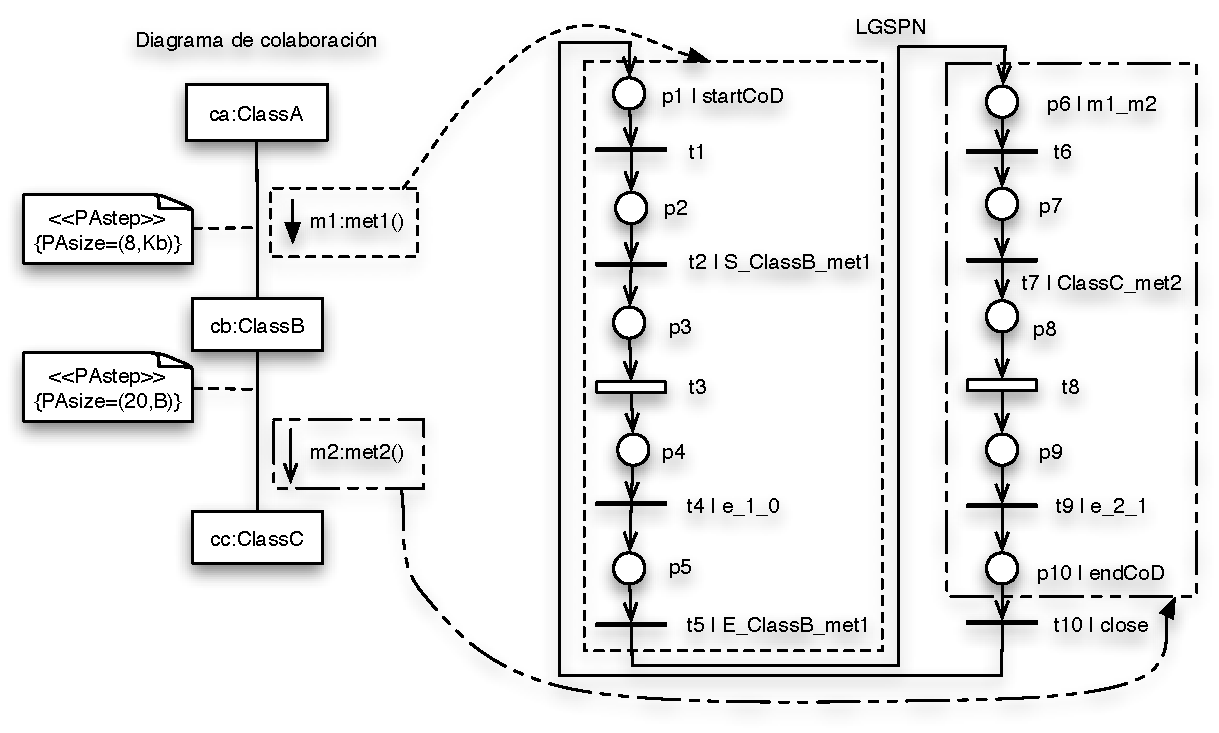
\includegraphics[scale=0.75]{translation.pdf}
		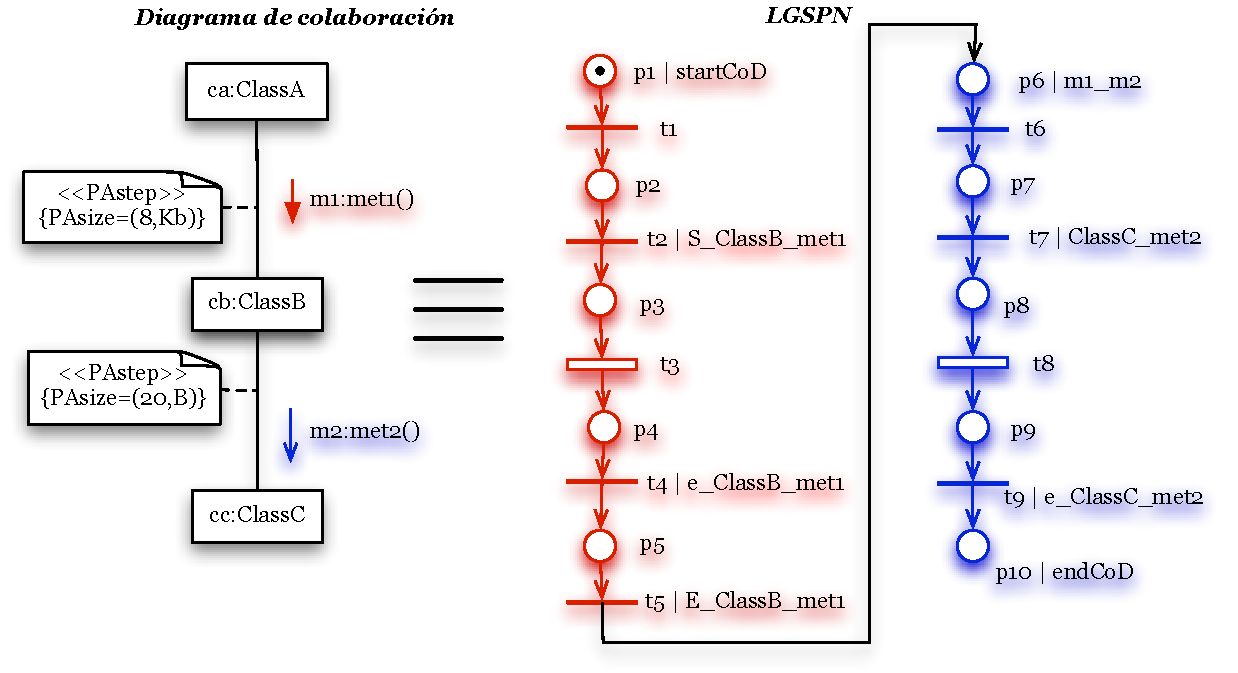
\includegraphics[scale=0.77]{translationColored.pdf}
	\end{center}
	\caption{Representaci�n del resultado del proceso de traducci�n.}
	\label{fig:traduccion}
\end{figure}

El proceso de traducci�n de un diagrama de colaboraci�n, se basa en la traducci�n por separado de cada uno de los mensajes que componen la colaboraci�n. 

Esta traducci�n ser� diferente dependiendo de los elementos que caractericen a ese mensaje, cada mensaje generar� una peque�a red que deber� ser fusionada con la RdP generada por el mensaje anterior, una vez finalizada la composici�n de las RdP's asociadas a los mensajes habremos obtenido como resultado una RdP que representar� el comportamiento modelado por nuestro diagrama. 

La informaci�n necesaria para determinar la traducci�n de un mensaje ser� recibida a trav�s de un fichero XMI, que es el formato en el que se almacenar� la informaci�n de nuestro modelo, de aqu� tomaremos si el mensaje es s�ncrono o as�ncrono, si ha sido anotado especificando su tama�o o no, as� como otras cuestiones de menor importancia.

En la figura \ref{fig:traduccion} observamos que el mensaje {\em m1} (coloreado en {\bf rojo}) tiene una traducci�n diferente (RdP {\bf roja}) al mensaje {\em m2} (en {\bf azul}, como su RdP), el primero es s�ncrono, (lo cual viene reflejado por la representaci�n de su flecha, los mensajes s�ncronos se representan por una flecha con la punta rellena) y est� etiquetado con un tama�o, el segundo es as�ncrono, (por lo que est� representado por una flecha con punta sin rellenar).

Este esquema representa la salida del traductor que he implementado ante ese diagrama de colaboraci�n,  adem�s tenemos que se�alar que el traductor soporta cualquier elemento que pueda ser modelado dentro de un diagrama de colaboraci�n por ArgoUML, y ha sido integrado con �xito formando ya parte de ArgoSPE. Con lo que consideramos como cumplido el objetivo de conseguir la traducci�n de estos diagramas.

\subsection{Composici�n}

El proceso de composici�n es dif�cil de explicar sin ayudarnos de complicadas f�rmulas, por lo que vamos a mostrar a continuaci�n un esquema que muestra el resultado final para intentar facilitar la comprensi�n del mismo:

\begin{figure}[H]
%\begin{figure}[hbt]
	\begin{center}
		%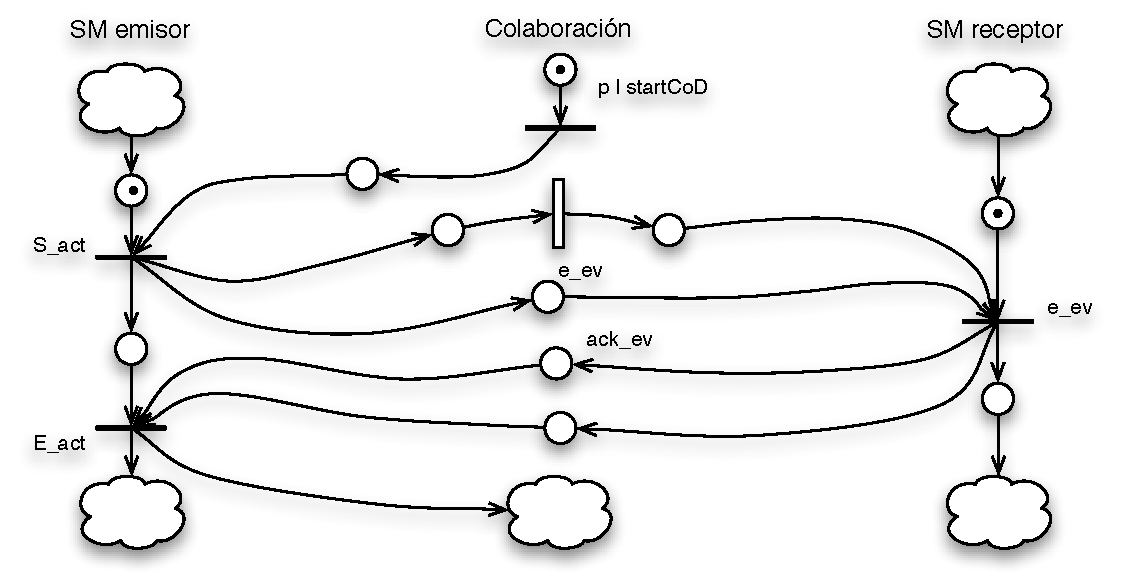
\includegraphics[scale=0.72]{merge.pdf}
		%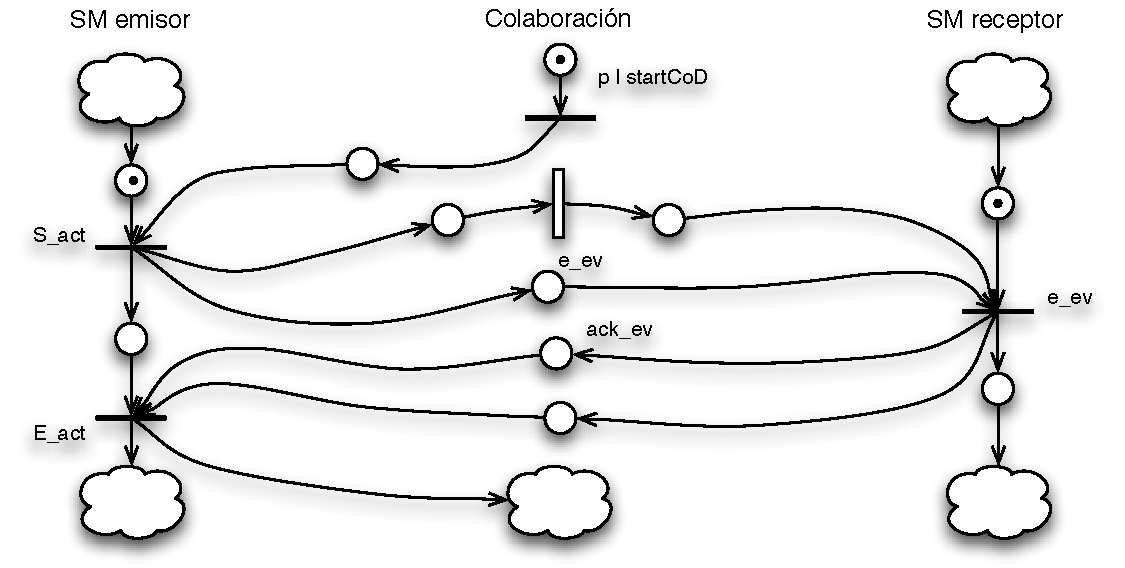
\includegraphics[scale=0.72]{merge2.pdf}
		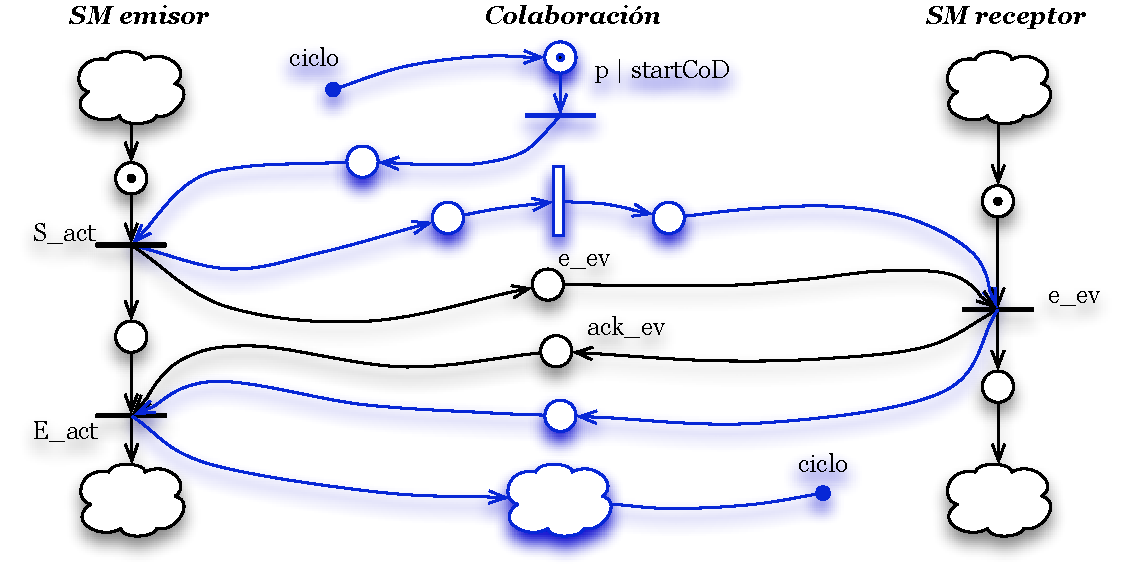
\includegraphics[scale=0.72]{mergeColored.pdf}
	\end{center}
	\caption{Composici�n entre m�quinas de estado y diagramas de colaboraci�n.}
	\label{fig:merge}
\end{figure}

Al observar el gr�fico anterior con atenci�n tenemos que fijarnos que existen varios elementos diferenciados, en la parte izquierda tenemos la RdP obtenida de la traducci�n de la m�quina de estados de la clase que ha generado el mensaje, el cual deber� estar representado en el diagrama de colaboraci�n, en la parte derecha estar� la RdP de la m�quina de estados de la clase que recibe el mensaje. Por �ltimo en la parte central aparece un fragmento de la RdP generada al traducir el diagrama de colaboraci�n.

En relaci�n con el dibujo tenemos que destacar que se ha considerado oportuno resaltar, colore�ndola de {\bf azul}, la RdP generada por el mensaje (del diagrama de colaboraci�n), con el fin de facilitar la comprensi�n del esquema por parte del lector. Con esta medida tambi�n conseguimos aislar el resultado producido por la composici�n de las RdP de las m�quinas de estado, las cuales, como se puede observar tienen en los eventos de igual nombre su nexo de uni�n. Este es el mismo mecanismo utilizado en el gr�fico de la traducci�n para diferenciar la RdP generada por cada uno de los mensajes.

Para entender el porqu� de este proceso, tenemos que explicar una serie de cuestiones, lo primero de todo es que las clases son los elementos que definen la estructura de nuestro dise�o, la m�quina de estados de cada una de ellas modela la din�mica seguida por una instancia suya, por lo tanto el comportamiento del sistema queda descrito gracias a todas las m�quinas de estados de las clases que participan en nuestro modelo.

Hasta ahora nuestra herramienta lo que hac�a era traducir las m�quinas de estados de un sistema y fusionarlas, con lo cual se obten�a un RdP gigantesca que caracterizaba el comportamiento global de nuestro sistema.

Los diagramas de colaboraci�n reflejan las interacciones que realizan unas determinadas clases con otras definiendo un escenario concreto para nuestro dise�o, es como si sacaramos una foto de como trabajan las clases para llevar a cabo una tarea.

Entonces al traducir el diagrama de colaboraci�n a RdP y fusionar esta red con la RdP completa de nuestro sistema, obtenemos una red que describir� el comportamiento del sistema completo en una determinada situaci�n (o escenario), que viene a ser la definida por nuestro diagrama.

Para lograr una perfecta composici�n entre las RdP anteriores, se tuvieron que realizar una serie de modificaciones en la traducci�n de las m�quinas de estados, debido a que las etiquetas generadas por las RdP, tanto de las referidas a los diagramas de estados como de las del diagrama de colaboraci�n, no eran iguales, condici�n sin la cual no se puede realizar la composici�n. Adem�s cont�bamos con problema a�adido de que GreatSPN tiene una longitud relativamente peque�a para almacenar las etiquetas, lo que nos oblig� a definir un formato que fuera lo suficientemente peque�o y que adem�s fuera �nico para cada uno de los elementos que representara.

Una vez subsanados todos los problemas simplemente tenemos que pasar las RdP generadas a {\bf algebra}, (paquete que acompa�a al programa GreatSPN y aporta la composici�n de GSPN's y la elminaci�n de etiquetas dentro de las redes), el cual ser� el encargado final de realizar la composici�n. Este programa funciona en l�nea comandos y la llamada ser�a algo parecido a esto:

\begin{center}
\verb	! rdp99:~/ algebra -no_ba net1 net2 t eti_file net12 1 !
\end{center}

El primer par�metro {\em --no\_ba} evita que los arcos sin destino o sin origen (en definitiva, rotos) sean dibujados en la red final. El fichero de etiquetas almacenar� todas las etiquetas de los elementos que tendr�n que fusionarse. Debemos mencionar adem�s que la {\em {\bf t}} que aparece como par�metro, se refiere a que la composici�n ser� meramente de transiciones ya que es lo �nico que se precisa en nuestro caso.

El �ltimo par�metro que acompa�a a la herramienta es un n�mero, en nuestro caso el 1, que ser� utilizado para indicar la colocaci�n final de las RdP dentro del fichero resultado, el 1 significa que se colocar�n horizontalmente, de izquierda a derecha, y si hubi�ramos utilizado el 2 la ordenaci�n hubiera sido vertical.

Como es l�gico {\em net1} y {\em net2} representar�n los ficheros en los que se encuentran las RdP's que queremos fusionar, y {\em net12} ser� el nombre del fichero en el que queremos que se almacene el resultado de la composici�n.

Una �ltima cuesti�n que no se ha mencionado anteriormente es el hecho de que ha resultado especialmente dif�cil la implementaci�n, tanto de la traducci�n como de la composici�n, ya que deb�amos de mantener intacta la funcionalidad que ya era proporcionada por la herrramienta, as� que las modificaciones requiridas en el c�digo existente se han realizado como com�nmente se suele decir, {\em con pies de plomo}.

\subsection{Consulta}

Todo lo implementado anteriormente quedar�a sin sentido si no proporcion�semos alg�n modo de sacar partido de ello.

Pensando detenidamente, vemos que el objetivo de anotar nuestro modelo con caracter�sticas que definan las prestaciones de ciertos elementos, es el obtener una informaci�n que sea �til durante la fase de modelado a la persona que est� realizando el dise�o del sistema.

Una de las cuestiones m�s interesantes que podemos preguntarnos cuando estamos dise�ando un sistema ser�a, �cu�nto tiempo nos cuesta ejecutar una determinada tarea? Pues bien esa es la pregunta que podemos responder gracias al proceso de traducci�n y composici�n.

En nuestro caso vamos a denominar a la consulta que a�adimos a ArgoSPE, {\bf Response Time} y vendr� definida como el tiempo medio de respuesta de un escenario concreto, la consulta se podr�a decir que calcula el tiempo de respuesta del diagrama de colaboraci�n que define dicho escenario.

Para poder calcular esta caracter�stica en nuestro sistema fue preciso realizar unas peque�as transformaciones a la RdP que gener�bamos en el proceso de traducci�n, �stas implican crear una transici�n etiquetada como {\em close}, que har� de puente entre el lugar final de la RdP del diagrama de colaboraci�n y su lugar inicial, obteniendo de esta manera una red cerrada necesaria para el an�lisis en el estado estacionario.

\subsection{Pruebas}

Al finalizar cada una de las etapas de implementaci�n se pasaba a un per�odo de comprobaci�n, este proceso era de una gran importancia debido a que todas las partes depend�an las unas de las otras para su correcto funcionamiento.

Para comprobar el buen comportamiento del c�digo creado para realizar la traducci�n se ten�a que modelar ejemplos de sistemas, en ArgoUML, que cumplieran los requisitos necesarios para poder generar una RdP.

Estos requisitos pasaban por dise�ar, al menos dos clases, cada una con sus respectivos diagramas de estados, y en las que ten�amos que enviar y recibir al menos un evento, lo que quiere decir que, en una de las m�quinas de estados una acci�n ser�a la llamada de uno de los m�todos de la otra clase y en la m�quina de estados de la clase llamada recoger�amos la llamada, gracias al modelado del evento disparador (o trigger). Esta misma interacci�n era representada a su vez con un diagrama de colaboraci�n. Una vez ideado el sistema ten�amos que anotar el dise�o con las anotaciones conforme a la tabla \ref{tab:anotaciones}.

Con todo esto ya podr�amos generar una RdP para nuestro diagrama de colaboraci�n con nuestro traductor, la cual deber�a ser comparada con una RdP que hab�amos elaborado a mano previamente, con la estructura correcta.

Este mismo proceso tambi�n es seguido para la comprobaci�n del adecuado funcionamiento del c�digo de la composici�n, aunque en este caso se hace mucho m�s complicada la verificaci�n debido al gran n�mero de lugares y transiciones existentes en la red, recordemos que estamos formando una �nica red a partir de todas las RdP de las m�quinas de estado y de la del diagrama de colaboraci�n seleccionado.
 
 Con todo lo dicho queda claro que la realizaci�n de pruebas es una tarea bastante complicada.
 
\section{Valoraci�n del trabajo}

\subsection{Aplicaci�n del trabajo desarrollado}

Uno de los logros m�s significativos de este proyecto es la contribuci�n realizada a una aplicaci�n, ArgoSPE, que tiene como objetivo mejorar el proceso de desarrollo del software, introduciendo los criterios de prestaciones desde la fases iniciales del ciclo de vida del sistema, con el fin de ahorrar tiempo evitando dise�os que no cumplir�n los requisitos que nos hemos marcado.

No nos podemos olvidar que al mejorar ArgoSPE, tambi�n estamos posibilitando el aumento las caracter�sticas ofrecidas por ArgoUML, cuya versi�n 0.18.1 fue bajada 98.143 veces (datos hasta Agosto de 2005), todos estos usuarios al fin y al cabo son usuarios potenciales de nuestro m�dulo.

Es m�s, a pesar de sus deficiencias y de que a�n no existe una versi�n totalmente estable, ArgoUML es la herramienta CASE, gratuita y de c�digo libre, m�s utilizada en todo  el mundo.

\subsection{Trabajo futuro}

Una de las ventajas de haber trabajado en la mayor�a de las componentes que constituyen la aplicaci�n es que se tiene una visi�n global de la funcionalidad que ofrece y de las posibles mejoras que podr�an llegar a realizarse.

En mi opini�n sugerir nuevas funcionalidades para una aplicaci�n sin conocer, de una manera precisa, el estado de las funcionalidades que ahora mismo aporta no es algo razonable. Por este motivo la primera ampliaci�n que propondr�a ser�a la realizaci�n de un estudio del proceso de traducci�n, que refleje las situaciones que son tenidas en cuenta y las que no soporta.

Una vez realizado ese estudio, enfocar�a los esfuerzos en subsanar todos los defectos encontrados en la traducci�n, as� como la implementaci�n de cada nuevo aspecto que se han tenido en cuenta en el trabajo \cite{TSE}, ya que la considero un punto clave sobre el que se fundamenta el buen funcionamiento de nuestra herramienta.

Bas�ndonos ahora en el enfoque de ampliar la funcionalidad de ArgoSPE, cabe se�alar la realizaci�n de un estudio de herramientas CASE que puedan ser utilizadas con nuestro m�dulo. El objeto de cambiar ArgoUML por otra aplicaci�n no es otro que proporcionar un mayor abanico de diagramas con los que pueda trabajar nuestra herramienta, a la vez que contar con un mayor n�mero de elementos implementados dentro de cada tipo de diagrama.

Otra ampliaci�n que resultar�a de gran utilidad ser�a sustituir el formato de las RdP que genera el traductor, ya que actualmente las RdP se generan con formato GreatSPN, formato que no es est�ndar, por lo que limita la herramienta con la que podemos analizar las redes obtenidas. El mejor candidato como formato est�ndar de RdP es {\bf PNML} ({\bf P}etri {\bf N}et {\bf M}arkup {\bf L}anguage) \cite{PNML}.

Por supuesto la funcionalidad que ArgoSPE ofrece, viene dada por las consultas que proporcione sobre los modelos de nuestros sistemas, por eso consideramos una buena opci�n a�adir m�s consultas a las ya implementadas por nuestra aplicaci�n.

Para finalizar me gustar�a proponer la investigaci�n de las caracter�sticas menos documentadas de esta aplicaci�n, lo cual implicar�a la lectura detallada de todos los documentos relacionados con ella que existen, como art�culos memorias de proyectos fin de carrera y dem�s y tratar de aclarar todo aquello que sea susceptible de ser necesitado por futuros desarrolladores. 

\section{Conclusiones personales}

Como resultado de este proyecto la principal conclusi�n que se puede extraer es lo valioso que resultan  la  experiencia y los conocimientos adquiridos a lo largo de su desarrollo.  

Por un lado he conseguido incrementar ampliamente mis conocimientos de Java, uno de los  lenguajes m�s extendidos en la actualidad. Adem�s he asentado y aumentado mi entendimiento sobre un est�ndar tan extendido e importante como es UML. Por otra parte tambi�n he sido capaz poner en pr�ctica algunos de los conocimientos adquiridos a lo largo de mi per�odo de formaci�n.

Por otro lado he aprendido a utilizar con soltura herramientas b�sicas en el desarrollo  de proyectos como CVS, Ant (para desarrollo de Java) y otras herramientas proporcionadas por el sistema operativo GNU/Linux, adem�s del perfeccionamiento en el manejo del editor de textos Vim.

La envergadura de este tipo de trabajos me ha aportado tambi�n soltura a la hora de planificar, documentar  y gestionar las diferentes etapas que lo compon�an.

Un concepto importante que he aprendido es que una adecuada organizaci�n inicial,  una  correcta  planificaci�n  y  unos  conocimientos  previos  bien asentados (no necesarios pero desde luego deseables) son elementos muy a tener en cuenta ya que facilitan en gran medida el trabajo desarrollado a posteriori y ahorran gran cantidad de tiempo y esfuerzo.

Gracias a la observaci�n de otros proyectos como ArgoUML se han adquirido nociones de c�mo se organiza y planifica un proyecto software, en el cual colaboran decenas de personas (siempre dentro del marco de un proyecto de c�digo libre). El hecho de que toda la gesti�n del proyecto se realice v�a web le da a�n m�s  valor a este asunto. 

En �ltimo  lugar me gustar�a  expresar  que  estoy  profundamente  satisfecho  con  el  resultado de este proyecto y espero que los conocimientos y mecanismos aprendidos durante su desarrollo me resulten muy �tiles en un, esperemos pr�ximo, entorno laboral.
	%\chapter{Resultados y conclusiones}
\label{chap:res}
\section{Dificultades encontradas}

Cumplir los objetivos marcados al inicio de este trabajo no ha sido un tarea precisamente sencilla. En esta secci�n se har� una breve descripci�n de las dificultades y problemas que nos hemos encontrado y que han sido superados.

Este proyecto utiliza y ampl�a una herramienta ya implementada, ArgoSPE. Durante mi per�odo de formaci�n en la carrera se nos ha inculcado la creencia de que la {\bf comprensi�n de c�digo ajeno}, es una de las tareas m�s complicadas con las que nos podemos enfrentar, de ah� que ayude enormemente una buena documentaci�n del mismo. En nuestro caso nos hemos encontrado con partes que no han sido adecuadamente documentadas, lo que ha llevado a realizar una gran inversi�n de tiempo para comprender dicha implementaci�n.

El primer obst�culo que hemos tenido que salvar fue la comprensi�n de una {\bf parte te�rica realmente compleja}. Para empezar tuvimos que estudiar el est�ndar UML 1.4.2\footnote{El documento de sus especificaciones t�cnicas cuenta con 736 p�ginas de extensi�n.} que nos ayudar�a a poder modelar los ejemplos que m�s tarde utilizar�amos para la comprobaci�n del funcionamiento de nuestra aportaci�n. 

M�s adelante adquirimos los conceptos necesarios para modelar las prestaciones que deber�amos anotar en nuestros modelos, gracias al UML-SPT\footnote{Este documento abarca un total de 232 p�ginas.}, documento que encierra cantidad de conceptos con un alto grado de abstracci�n.

Por �ltimo, y no por ello lo m�s simple, entender la teor�a que rige la traducci�n de diagramas UML al dominio de las LGSPN's conlleva un gran esfuerzo, basta decir que es el trabajo investigado en la tesis de mi director \cite{Merse-PhD}, y que adem�s ha suscitado numerosos art�culos de investigaci�n.

Aprender a utilizar la herramienta ArgoSPE no ha resultado algo trivial, el motivo principal es la falta de documentaci�n en relaci�n a su uso, principalmente en el apartado de la anotaci�n de los diagramas UML, tema indispensable cuando tratamos de comprobar el funcionamiento del programa.

La naturaleza de las ampliaciones que he tenido que realizar dentro de ArgoSPE me han obligado a meterme de lleno con cada una de las partes de la arquitectura que compone la aplicaci�n, lo cual me ha supuesto observar con detalle la mayor�a del c�digo implementado en cada uno de los {\bf 167 ficheros fuente} que constituyen nuestra herramienta.

Unido a esto ha sido necesario realizar modificaciones sobre partes del c�digo que ya estaban implementadas, estas modificaciones han sido motivadas fundamentalmente por dos razones, la primera ha sido la correcci�n de algunos errores en la traducci�n de las m�quinas de estado, errores que ser�n explicados en los anexos con detalle. Y la segunda fue la transformaci�n de la traducci�n de los diagramas de estado para posibilitar la composici�n entre las RdP's resultantes. Como es comprensible esto ha llevado al estudio tanto te�rico como pr�ctico del proceso de traducci�n de estos diagramas.

\section{Trabajo realizado}
\label{sec:trabajo}
Para lograr alcanzar los objetivos marcados al principio de este trabajo (secci�n \ref{sec:objetivos}) hemos tenido que realizar una dura labor implementando tanto la traducci�n, como la composici�n, sin olvidarnos de la consulta a nivel UML. Los resultados obtenidos son explicados a continuaci�n.

\subsection{Traducci�n}
\label{subsec:traduccion}

Como hemos comentado con anterioridad la traducci�n consiste en el paso de un modelo en UML, en este caso, de los diagramas de colaboraci�n, al dominio de las LGSPN's. Vamos a representar en un dibujo la relaci�n que existe entre los dos modelos:
%\begin{figure}[H]
\begin{figure}[hbt]
	\begin{center}
		%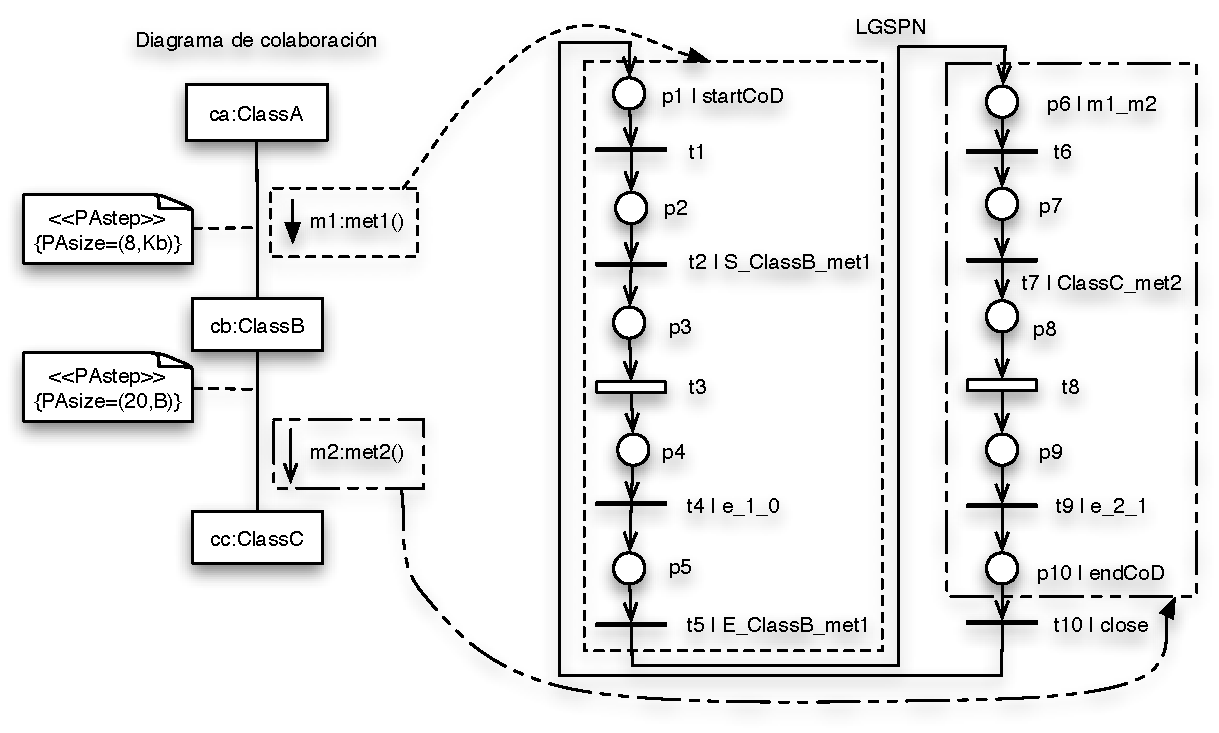
\includegraphics[scale=0.75]{translation.pdf}
		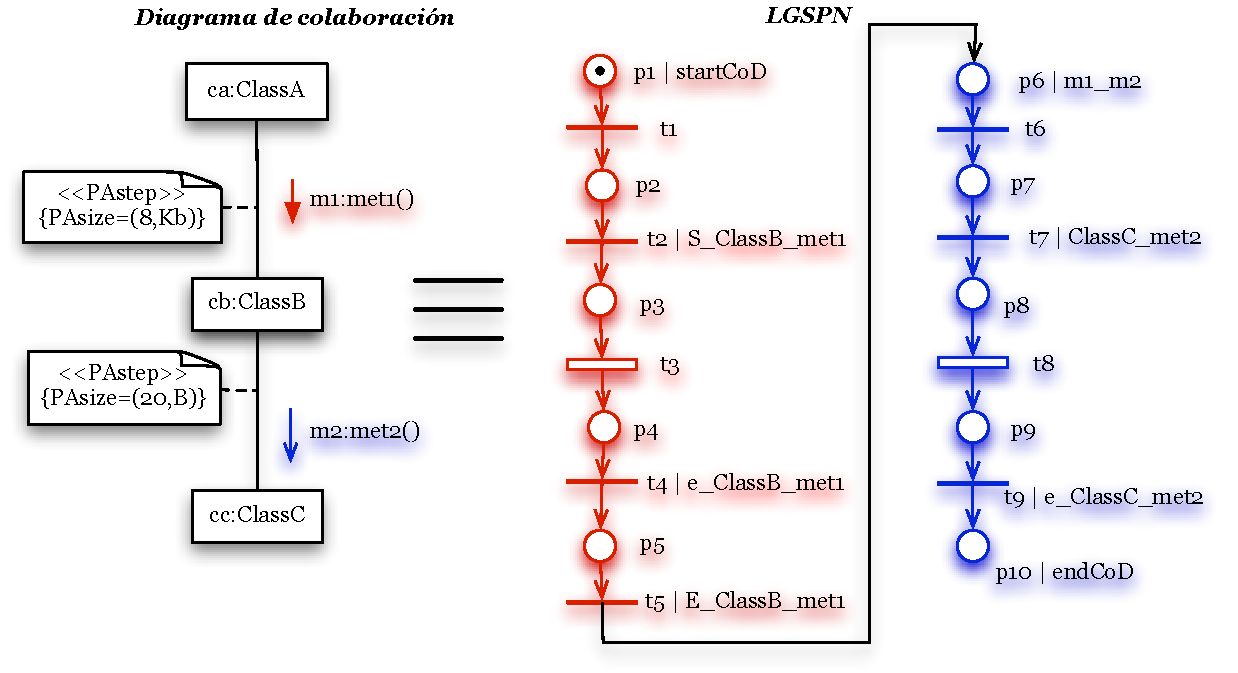
\includegraphics[scale=0.77]{translationColored.pdf}
	\end{center}
	\caption{Representaci�n del resultado del proceso de traducci�n.}
	\label{fig:traduccion}
\end{figure}

El proceso de traducci�n de un diagrama de colaboraci�n, se basa en la traducci�n por separado de cada uno de los mensajes que componen la colaboraci�n. 

Esta traducci�n ser� diferente dependiendo de los elementos que caractericen a ese mensaje, cada mensaje generar� una peque�a red que deber� ser fusionada con la RdP generada por el mensaje anterior, una vez finalizada la composici�n de las RdP's asociadas a los mensajes habremos obtenido como resultado una RdP que representar� el comportamiento modelado por nuestro diagrama. 

La informaci�n necesaria para determinar la traducci�n de un mensaje ser� recibida a trav�s de un fichero XMI, que es el formato en el que se almacenar� la informaci�n de nuestro modelo, de aqu� tomaremos si el mensaje es s�ncrono o as�ncrono, si ha sido anotado especificando su tama�o o no, as� como otras cuestiones de menor importancia.

En la figura \ref{fig:traduccion} observamos que el mensaje {\em m1} (coloreado en {\bf rojo}) tiene una traducci�n diferente (RdP {\bf roja}) al mensaje {\em m2} (en {\bf azul}, como su RdP), el primero es s�ncrono, (lo cual viene reflejado por la representaci�n de su flecha, los mensajes s�ncronos se representan por una flecha con la punta rellena) y est� etiquetado con un tama�o, el segundo es as�ncrono, (por lo que est� representado por una flecha con punta sin rellenar).

Este esquema representa la salida del traductor que he implementado ante ese diagrama de colaboraci�n,  adem�s tenemos que se�alar que el traductor soporta cualquier elemento que pueda ser modelado dentro de un diagrama de colaboraci�n por ArgoUML, y ha sido integrado con �xito formando ya parte de ArgoSPE. Con lo que consideramos como cumplido el objetivo de conseguir la traducci�n de estos diagramas.

\subsection{Composici�n}

El proceso de composici�n es dif�cil de explicar sin ayudarnos de complicadas f�rmulas, por lo que vamos a mostrar a continuaci�n un esquema que muestra el resultado final para intentar facilitar la comprensi�n del mismo:

\begin{figure}[H]
%\begin{figure}[hbt]
	\begin{center}
		%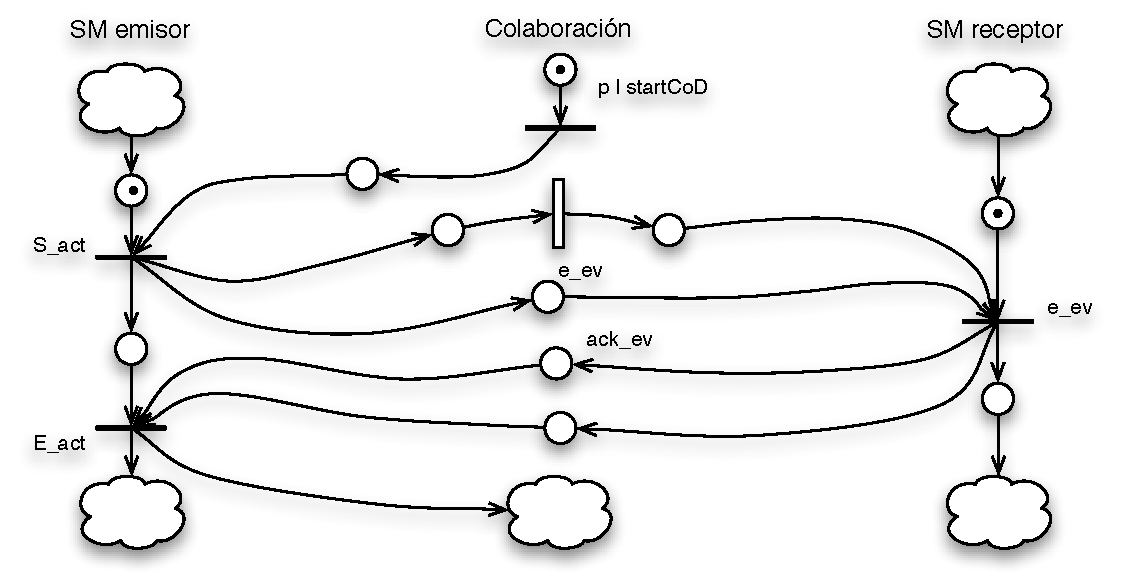
\includegraphics[scale=0.72]{merge.pdf}
		%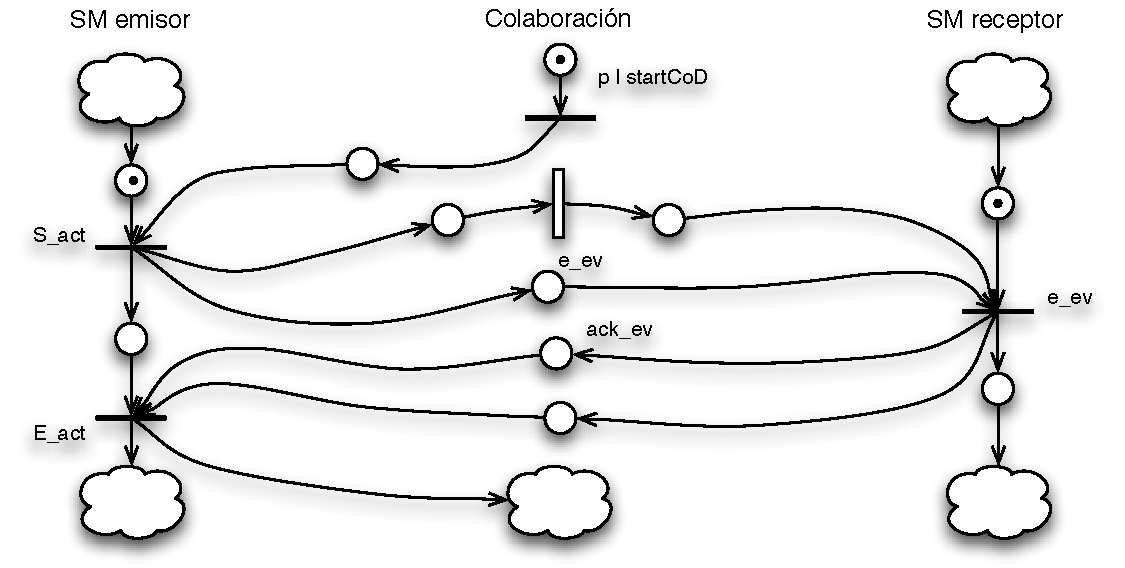
\includegraphics[scale=0.72]{merge2.pdf}
		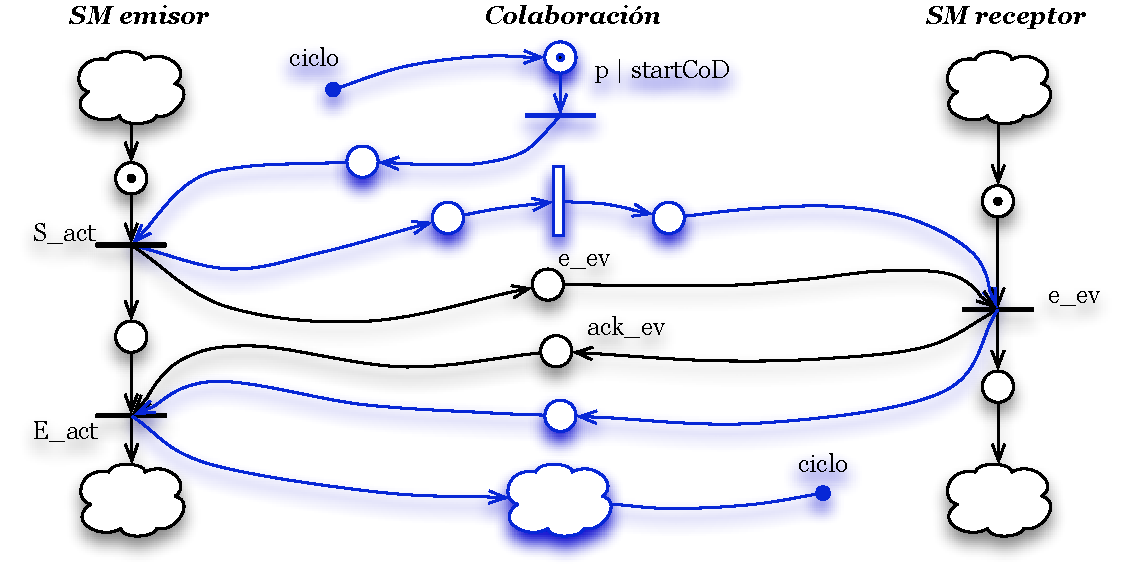
\includegraphics[scale=0.72]{mergeColored.pdf}
	\end{center}
	\caption{Composici�n entre m�quinas de estado y diagramas de colaboraci�n.}
	\label{fig:merge}
\end{figure}

Al observar el gr�fico anterior con atenci�n tenemos que fijarnos que existen varios elementos diferenciados, en la parte izquierda tenemos la RdP obtenida de la traducci�n de la m�quina de estados de la clase que ha generado el mensaje, el cual deber� estar representado en el diagrama de colaboraci�n, en la parte derecha estar� la RdP de la m�quina de estados de la clase que recibe el mensaje. Por �ltimo en la parte central aparece un fragmento de la RdP generada al traducir el diagrama de colaboraci�n.

En relaci�n con el dibujo tenemos que destacar que se ha considerado oportuno resaltar, colore�ndola de {\bf azul}, la RdP generada por el mensaje (del diagrama de colaboraci�n), con el fin de facilitar la comprensi�n del esquema por parte del lector. Con esta medida tambi�n conseguimos aislar el resultado producido por la composici�n de las RdP de las m�quinas de estado, las cuales, como se puede observar tienen en los eventos de igual nombre su nexo de uni�n. Este es el mismo mecanismo utilizado en el gr�fico de la traducci�n para diferenciar la RdP generada por cada uno de los mensajes.

Para entender el porqu� de este proceso, tenemos que explicar una serie de cuestiones, lo primero de todo es que las clases son los elementos que definen la estructura de nuestro dise�o, la m�quina de estados de cada una de ellas modela la din�mica seguida por una instancia suya, por lo tanto el comportamiento del sistema queda descrito gracias a todas las m�quinas de estados de las clases que participan en nuestro modelo.

Hasta ahora nuestra herramienta lo que hac�a era traducir las m�quinas de estados de un sistema y fusionarlas, con lo cual se obten�a un RdP gigantesca que caracterizaba el comportamiento global de nuestro sistema.

Los diagramas de colaboraci�n reflejan las interacciones que realizan unas determinadas clases con otras definiendo un escenario concreto para nuestro dise�o, es como si sacaramos una foto de como trabajan las clases para llevar a cabo una tarea.

Entonces al traducir el diagrama de colaboraci�n a RdP y fusionar esta red con la RdP completa de nuestro sistema, obtenemos una red que describir� el comportamiento del sistema completo en una determinada situaci�n (o escenario), que viene a ser la definida por nuestro diagrama.

Para lograr una perfecta composici�n entre las RdP anteriores, se tuvieron que realizar una serie de modificaciones en la traducci�n de las m�quinas de estados, debido a que las etiquetas generadas por las RdP, tanto de las referidas a los diagramas de estados como de las del diagrama de colaboraci�n, no eran iguales, condici�n sin la cual no se puede realizar la composici�n. Adem�s cont�bamos con problema a�adido de que GreatSPN tiene una longitud relativamente peque�a para almacenar las etiquetas, lo que nos oblig� a definir un formato que fuera lo suficientemente peque�o y que adem�s fuera �nico para cada uno de los elementos que representara.

Una vez subsanados todos los problemas simplemente tenemos que pasar las RdP generadas a {\bf algebra}, (paquete que acompa�a al programa GreatSPN y aporta la composici�n de GSPN's y la elminaci�n de etiquetas dentro de las redes), el cual ser� el encargado final de realizar la composici�n. Este programa funciona en l�nea comandos y la llamada ser�a algo parecido a esto:

\begin{center}
\verb	! rdp99:~/ algebra -no_ba net1 net2 t eti_file net12 1 !
\end{center}

El primer par�metro {\em --no\_ba} evita que los arcos sin destino o sin origen (en definitiva, rotos) sean dibujados en la red final. El fichero de etiquetas almacenar� todas las etiquetas de los elementos que tendr�n que fusionarse. Debemos mencionar adem�s que la {\em {\bf t}} que aparece como par�metro, se refiere a que la composici�n ser� meramente de transiciones ya que es lo �nico que se precisa en nuestro caso.

El �ltimo par�metro que acompa�a a la herramienta es un n�mero, en nuestro caso el 1, que ser� utilizado para indicar la colocaci�n final de las RdP dentro del fichero resultado, el 1 significa que se colocar�n horizontalmente, de izquierda a derecha, y si hubi�ramos utilizado el 2 la ordenaci�n hubiera sido vertical.

Como es l�gico {\em net1} y {\em net2} representar�n los ficheros en los que se encuentran las RdP's que queremos fusionar, y {\em net12} ser� el nombre del fichero en el que queremos que se almacene el resultado de la composici�n.

Una �ltima cuesti�n que no se ha mencionado anteriormente es el hecho de que ha resultado especialmente dif�cil la implementaci�n, tanto de la traducci�n como de la composici�n, ya que deb�amos de mantener intacta la funcionalidad que ya era proporcionada por la herrramienta, as� que las modificaciones requiridas en el c�digo existente se han realizado como com�nmente se suele decir, {\em con pies de plomo}.

\subsection{Consulta}

Todo lo implementado anteriormente quedar�a sin sentido si no proporcion�semos alg�n modo de sacar partido de ello.

Pensando detenidamente, vemos que el objetivo de anotar nuestro modelo con caracter�sticas que definan las prestaciones de ciertos elementos, es el obtener una informaci�n que sea �til durante la fase de modelado a la persona que est� realizando el dise�o del sistema.

Una de las cuestiones m�s interesantes que podemos preguntarnos cuando estamos dise�ando un sistema ser�a, �cu�nto tiempo nos cuesta ejecutar una determinada tarea? Pues bien esa es la pregunta que podemos responder gracias al proceso de traducci�n y composici�n.

En nuestro caso vamos a denominar a la consulta que a�adimos a ArgoSPE, {\bf Response Time} y vendr� definida como el tiempo medio de respuesta de un escenario concreto, la consulta se podr�a decir que calcula el tiempo de respuesta del diagrama de colaboraci�n que define dicho escenario.

Para poder calcular esta caracter�stica en nuestro sistema fue preciso realizar unas peque�as transformaciones a la RdP que gener�bamos en el proceso de traducci�n, �stas implican crear una transici�n etiquetada como {\em close}, que har� de puente entre el lugar final de la RdP del diagrama de colaboraci�n y su lugar inicial, obteniendo de esta manera una red cerrada necesaria para el an�lisis en el estado estacionario.

\subsection{Pruebas}

Al finalizar cada una de las etapas de implementaci�n se pasaba a un per�odo de comprobaci�n, este proceso era de una gran importancia debido a que todas las partes depend�an las unas de las otras para su correcto funcionamiento.

Para comprobar el buen comportamiento del c�digo creado para realizar la traducci�n se ten�a que modelar ejemplos de sistemas, en ArgoUML, que cumplieran los requisitos necesarios para poder generar una RdP.

Estos requisitos pasaban por dise�ar, al menos dos clases, cada una con sus respectivos diagramas de estados, y en las que ten�amos que enviar y recibir al menos un evento, lo que quiere decir que, en una de las m�quinas de estados una acci�n ser�a la llamada de uno de los m�todos de la otra clase y en la m�quina de estados de la clase llamada recoger�amos la llamada, gracias al modelado del evento disparador (o trigger). Esta misma interacci�n era representada a su vez con un diagrama de colaboraci�n. Una vez ideado el sistema ten�amos que anotar el dise�o con las anotaciones conforme a la tabla \ref{tab:anotaciones}.

Con todo esto ya podr�amos generar una RdP para nuestro diagrama de colaboraci�n con nuestro traductor, la cual deber�a ser comparada con una RdP que hab�amos elaborado a mano previamente, con la estructura correcta.

Este mismo proceso tambi�n es seguido para la comprobaci�n del adecuado funcionamiento del c�digo de la composici�n, aunque en este caso se hace mucho m�s complicada la verificaci�n debido al gran n�mero de lugares y transiciones existentes en la red, recordemos que estamos formando una �nica red a partir de todas las RdP de las m�quinas de estado y de la del diagrama de colaboraci�n seleccionado.
 
 Con todo lo dicho queda claro que la realizaci�n de pruebas es una tarea bastante complicada.
 
\section{Valoraci�n del trabajo}

\subsection{Aplicaci�n del trabajo desarrollado}

Uno de los logros m�s significativos de este proyecto es la contribuci�n realizada a una aplicaci�n, ArgoSPE, que tiene como objetivo mejorar el proceso de desarrollo del software, introduciendo los criterios de prestaciones desde la fases iniciales del ciclo de vida del sistema, con el fin de ahorrar tiempo evitando dise�os que no cumplir�n los requisitos que nos hemos marcado.

No nos podemos olvidar que al mejorar ArgoSPE, tambi�n estamos posibilitando el aumento las caracter�sticas ofrecidas por ArgoUML, cuya versi�n 0.18.1 fue bajada 98.143 veces (datos hasta Agosto de 2005), todos estos usuarios al fin y al cabo son usuarios potenciales de nuestro m�dulo.

Es m�s, a pesar de sus deficiencias y de que a�n no existe una versi�n totalmente estable, ArgoUML es la herramienta CASE, gratuita y de c�digo libre, m�s utilizada en todo  el mundo.

\subsection{Trabajo futuro}

Una de las ventajas de haber trabajado en la mayor�a de las componentes que constituyen la aplicaci�n es que se tiene una visi�n global de la funcionalidad que ofrece y de las posibles mejoras que podr�an llegar a realizarse.

En mi opini�n sugerir nuevas funcionalidades para una aplicaci�n sin conocer, de una manera precisa, el estado de las funcionalidades que ahora mismo aporta no es algo razonable. Por este motivo la primera ampliaci�n que propondr�a ser�a la realizaci�n de un estudio del proceso de traducci�n, que refleje las situaciones que son tenidas en cuenta y las que no soporta.

Una vez realizado ese estudio, enfocar�a los esfuerzos en subsanar todos los defectos encontrados en la traducci�n, as� como la implementaci�n de cada nuevo aspecto que se han tenido en cuenta en el trabajo \cite{TSE}, ya que la considero un punto clave sobre el que se fundamenta el buen funcionamiento de nuestra herramienta.

Bas�ndonos ahora en el enfoque de ampliar la funcionalidad de ArgoSPE, cabe se�alar la realizaci�n de un estudio de herramientas CASE que puedan ser utilizadas con nuestro m�dulo. El objeto de cambiar ArgoUML por otra aplicaci�n no es otro que proporcionar un mayor abanico de diagramas con los que pueda trabajar nuestra herramienta, a la vez que contar con un mayor n�mero de elementos implementados dentro de cada tipo de diagrama.

Otra ampliaci�n que resultar�a de gran utilidad ser�a sustituir el formato de las RdP que genera el traductor, ya que actualmente las RdP se generan con formato GreatSPN, formato que no es est�ndar, por lo que limita la herramienta con la que podemos analizar las redes obtenidas. El mejor candidato como formato est�ndar de RdP es {\bf PNML} ({\bf P}etri {\bf N}et {\bf M}arkup {\bf L}anguage) \cite{PNML}.

Por supuesto la funcionalidad que ArgoSPE ofrece, viene dada por las consultas que proporcione sobre los modelos de nuestros sistemas, por eso consideramos una buena opci�n a�adir m�s consultas a las ya implementadas por nuestra aplicaci�n.

Para finalizar me gustar�a proponer la investigaci�n de las caracter�sticas menos documentadas de esta aplicaci�n, lo cual implicar�a la lectura detallada de todos los documentos relacionados con ella que existen, como art�culos memorias de proyectos fin de carrera y dem�s y tratar de aclarar todo aquello que sea susceptible de ser necesitado por futuros desarrolladores. 

\section{Conclusiones personales}

Como resultado de este proyecto la principal conclusi�n que se puede extraer es lo valioso que resultan  la  experiencia y los conocimientos adquiridos a lo largo de su desarrollo.  

Por un lado he conseguido incrementar ampliamente mis conocimientos de Java, uno de los  lenguajes m�s extendidos en la actualidad. Adem�s he asentado y aumentado mi entendimiento sobre un est�ndar tan extendido e importante como es UML. Por otra parte tambi�n he sido capaz poner en pr�ctica algunos de los conocimientos adquiridos a lo largo de mi per�odo de formaci�n.

Por otro lado he aprendido a utilizar con soltura herramientas b�sicas en el desarrollo  de proyectos como CVS, Ant (para desarrollo de Java) y otras herramientas proporcionadas por el sistema operativo GNU/Linux, adem�s del perfeccionamiento en el manejo del editor de textos Vim.

La envergadura de este tipo de trabajos me ha aportado tambi�n soltura a la hora de planificar, documentar  y gestionar las diferentes etapas que lo compon�an.

Un concepto importante que he aprendido es que una adecuada organizaci�n inicial,  una  correcta  planificaci�n  y  unos  conocimientos  previos  bien asentados (no necesarios pero desde luego deseables) son elementos muy a tener en cuenta ya que facilitan en gran medida el trabajo desarrollado a posteriori y ahorran gran cantidad de tiempo y esfuerzo.

Gracias a la observaci�n de otros proyectos como ArgoUML se han adquirido nociones de c�mo se organiza y planifica un proyecto software, en el cual colaboran decenas de personas (siempre dentro del marco de un proyecto de c�digo libre). El hecho de que toda la gesti�n del proyecto se realice v�a web le da a�n m�s  valor a este asunto. 

En �ltimo  lugar me gustar�a  expresar  que  estoy  profundamente  satisfecho  con  el  resultado de este proyecto y espero que los conocimientos y mecanismos aprendidos durante su desarrollo me resulten muy �tiles en un, esperemos pr�ximo, entorno laboral.
	
	\part{Anexos}
	
	\appendix
	
	\chapter{An�lisis de UML}
\label{chap:uml}
\section{Diagramas de estados}
Un {\bf diagrama de estados} se utiliza para modelar aspectos din�micos de un sistema. La mayor�a de las veces esto supone el modelado del comportamiento de objetos reactivos. Un {\bf objeto reactivo} es aqu�l para el que la mejor forma de caracterizar su comportamiento es se�alar cu�l es su respuesta a los eventos lanzados desde fuera de su contexto.

Los diagramas de estados pueden asociarse a las clases, los casos de uso, o a sistemas completos para visualizar, especificar, construir y documentar la din�mica de un objeto individual.  

Supongamos que hemos modelado una clase que representa un sistema de registro (login) de usuarios. El comportamiento din�mico de cada objeto que instancia dicha  clase se modela con el ejemplo de la figura \ref{fig:SC}, que adem�s nos sirve como ejemplo de la  notaci�n gr�fica empleada en un diagrama de estados:    
\begin{figure}[H]
	\begin{center}
		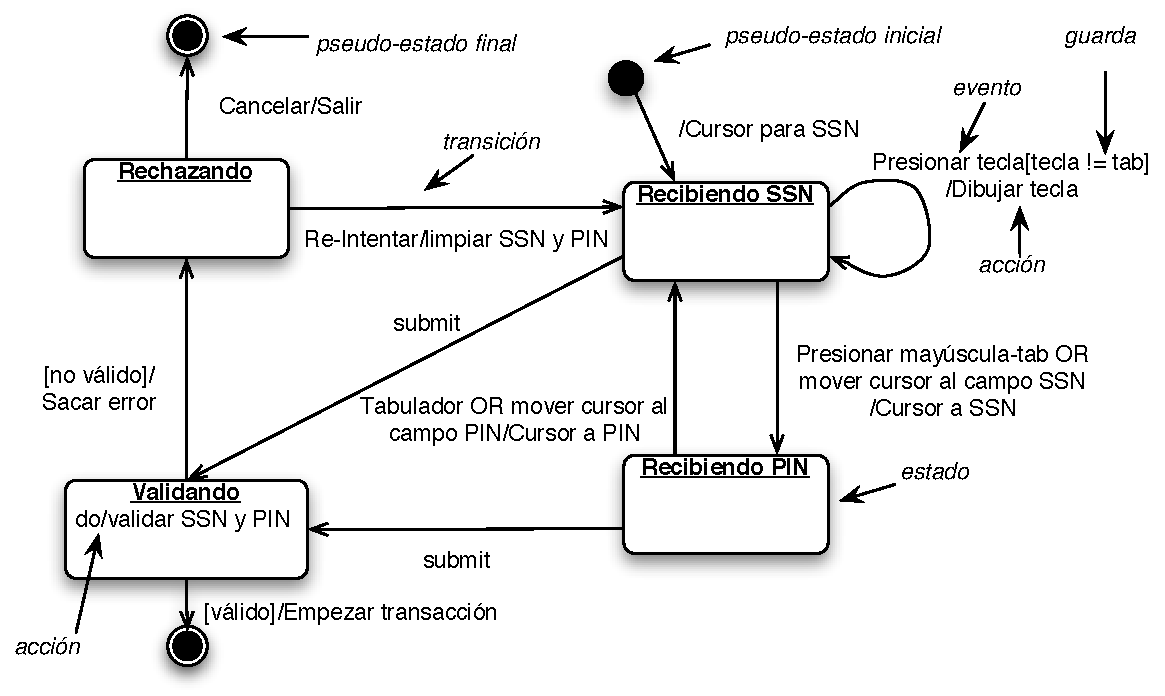
\includegraphics[scale=0.6]{SC.pdf}
	\end{center}
	\caption{Ejemplo de diagrama de estados.}
	\label{fig:SC}
\end{figure}

Tambi�n en este ejemplo vemos algunos de los elementos m�s representativos, las  relaciones que se establecen entre ellos y varios adornos. Los elementos m�s comunes dentro de un diagrama de estados son los estados y las  transiciones.

Un {\bf estado} es una condici�n o situaci�n en la vida de un objeto durante la cual  satisface alguna condici�n, realiza alguna actividad o espera alg�n evento. Cuando la  m�quina de estados de un objeto se encuentra en un estado dado, se dice que el objeto est�  en ese estado y que ese estado est� {\bf activo}. 

Un estado tiene varias partes: un nombre (cadena de texto que distingue al estado de  otros  estados),  {\bf acciones  de  entrada}  (acciones  ejecutadas  al  entrar  en  el  estado  e  identificadas con la palabra clave {\em entry}), {\bf acciones de salida} (acciones ejecutadas al salir de  un estado e identificadas con la palabra clave {\em exit}), {\bf transiciones internas} (transiciones que  se manejan sin causar un cambio en el estado), {\bf actividades} (actividades que son ejecutadas  mientras se encuentra activo el estado que las contiene y que se identifican con la palabra  clave {\em do}) y {\bf eventos diferidos} (lista de eventos que no se manejan en este estado sino que se  posponen y se a�aden a una cola para ser manejados por el objeto en otro estado).

Adem�s de los estados simples podemos encontrar otros tipos de estados como los  estados  compuestos,  los  estados {\bf de sincronizaci�n},  los  estados  de  subm�quina,  los  pseudoestados, etc.

En la figura del ejemplo vemos dos tipos de estado m�s muy comunes que son el {\bf estado inicial}, que indica el punto de comienzo por defecto para una m�quina de estados o  el subestado, y el {\bf estado final}, que indica que la ejecuci�n de la m�quina de estados o del  estado que lo contiene ha finalizado.

Los estados {\bf compuestos} son tambi�n elementos comunes de los diagramas de estados. Mientras que un estado simple no tiene una subestructura, un estado compuesto es  capaz de contener a otros estados. Los estados anidados dentro de un estado compuesto  reciben el nombre de subestados. Cuando un subestado est� activo,  tambi�n lo est� el  estado compuesto que lo contiene. Adem�s, los subestados se pueden anidar a cualquier  nivel.    

Una {\bf transici�n} es una relaci�n entre dos estados que indica que un objeto que est� en  el primer estado realizar� ciertas acciones y entrar� en el segundo estado cuando ocurra un  evento especificado y se satisfagan unas condiciones espec�ficas. Cuando se produce ese  cambio de estado se dice que la transici�n se ha disparado.  Una transici�n tiene cinco partes:

\begin{itemize}
\item {\bf Estado origen}: El estado afectado por la transici�n; si un objeto est� en el  estado origen,  una transici�n de salida puede dispararse cuando el objeto  reciba el evento de disparo de la transici�n, y si la condici�n de guarda,  si  la hay,  se satisface.
\item {\bf Evento de disparo}: el evento cuya recepci�n por el objeto que est� en el  estado  origen  provoca  el  disparo  de  la  transici�n  si  se  satisface  su  condici�n de guarda.
\item {\bf Condici�n de guarda}: Una expresi�n booleana que se eval�a cuando la  transici�n se activa por la recepci�n del evento de disparo; si la expresi�n  toma el valor cierto, la transici�n se puede disparar; si la expresi�n toma el valor falso,  la transici�n no se dispara y si no hay otra transici�n que  pueda ser disparada por el mismo evento, �ste se pierde.
\item {\bf Acci�n}:  Una  computaci�n  at�mica  ejecutable  que  puede  actuar  directamente  sobre  el  objeto  asociado  a  la  m�quina  de  estados,  e  indirectamente sobre otros objetos visibles al objeto.
\item {\bf Estado destino}: El estado activo tras completarse la transici�n.
\end{itemize} 

%\colorbox{red}{A�adir las partes que tiene Jose Luis S�nchez en el Anexo C}

\section{Diagramas de colaboraci�n}
%\section{Sem�ntica de los diagramas de colaboraci�n}
Un {\bf diagrama de colaboraci�n} es uno de los dos tipos de diagrama de interacci�n que podemos encontrar, �stos �ltimos est�n dedicados a describir c�mo colaboran un grupo de objetos para conseguir la realizaci�n de una tarea. En ellos se muestra los mensajes intercambiados entre los objetos dentro de un caso de uso, recogiendo de esta manera el comportamiento del mismo, o de un diagrama de clases.

Los dos tipos de diagramas de interacci�n muestran la colaboraci�n entre los objetos aunque cada uno  hace �nfasis en una cualidad diferente de esta relaci�n, as� por ejemplo los {\bf diagramas de secuencia}, que son los otros diagramas pertenecientes a este grupo, remarcan la ordenaci�n temporal de los mensajes, mostrando la secuencia de mensajes intercambiados a lo largo de la l�nea de vida de cada uno de los objetos participantes.

Por el contrario los diagramas de colaboraci�n enfatizan la organizaci�n estructural de los objetos que componen la interacci�n, en detrimento de la representaci�n del orden temporal de los mensajes, no obstante, se puede conocer la ordenaci�n de �stos simplemente fij�ndose en los n�meros de secuencia que aparecen representados en el diagrama. A partir de este punto vamos a centrarnos en el diagrama de colaboraci�n, ya que es el diagrama de interacci�n que es relevante para nuestro trabajo.

En el metamodelo de UML el paquete que define los elementos que utilizaremos en los diagramas de colaboraci�n, es el Collaborations package (o paquete de Colaboraciones), �ste se relaciona con otros paquetes que forman parte del metamodelo, siguiendo la estructura representada en la figura:

\begin{figure}[H]
	\begin{center}
		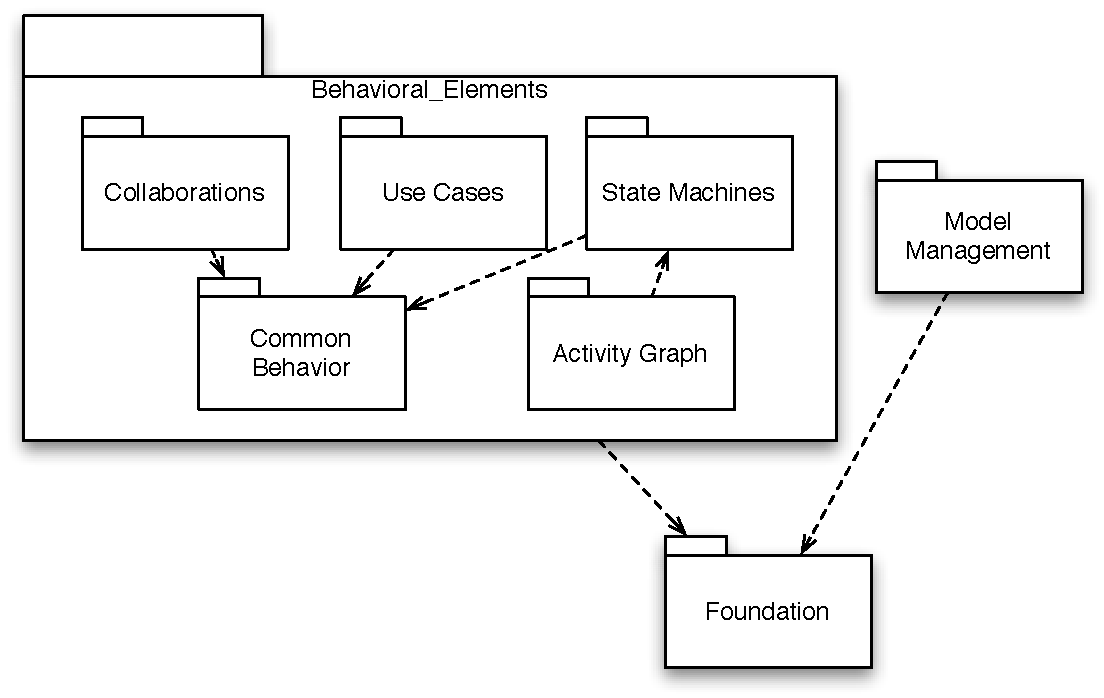
\includegraphics[scale=0.6]{UMLpackages.pdf}
	\end{center}
	\caption{Paquetes del metamodelo de UML.}
	\label{fig:metapackages}
\end{figure} 

El paquete {\bf Behavioral\_Elements} (Elementos de comportamiento) es una estructura que especifica el comportamiento din�mico. El paquete Collaborations, como vemos, forma parte de este super-paquete, y est� dividido en dos partes: la {\bf colaboraci�n} y la {\bf interacci�n}.

\begin{description}
\item[Colaboraci�n] define los roles que juegan (o los papeles representados por) un conjunto de instancias cuando realizan una tarea en particular, como una operaci�n o un caso de uso. 
\item[Interacci�n]  Es una colecci�n de comunicaciones producidas entre instancias, en las que se incluyen todos los tipos de formas en las cuales podemos afectar en una instancia, como la invocaci�n de una operaci�n, o la creaci�n y destrucci�n de �stas. Las comunicaciones est�n parcialemente ordenadas (en tiempo). Una interacci�n expresa un patr�n de comunicaci�n modelado por las instancias que representan los roles de una colaboraci�n.
\end{description}

%Si consigo hacer el glosario lo podremos quitar de aqui

\subsection{Interacciones}
Los elementos que forman parte de una interacci�n son los siguientes:
\begin{itemize}
\item {\bf Instancia} (objeto, valor de datos, instancia de un componente): es una entidad con una �nica identidad y para la cual tenemos un conjunto de operaciones que pueden ser aplicadas (o se�ales ser enviadas) y que tiene un estado que almacena los efectos de las operaciones.
\item {\bf Acci�n}: una especificaci�n de una sentencia ejecutable. Existen diferentes tipos de acciones que est�n predefinidas, por ejemplo acci�n de creaci�n, de llamada, de destrucci�n, y la acci�n no interpretada.
\item {\bf Est�mulo}: representa una comunicaci�n entre dos instancias. La notaci�n utilizada para definir un est�mulo es una flecha.
\item  {\bf Operaci�n}: una declaraci�n de un servicio que puede ser consultado desde una instancia para conseguir un comportamiento.
\item {\bf Se�al}: una especificaci�n de un est�mulo as�ncrono comunicado entre instancias.
\item {\bf Enlace}: una conexi�n entre instancias.
\end{itemize}

\subsection{Colaboraci�n}
Una colaboraci�n, a su vez, tambi�n est� constitu�da por un conjunto de artefactos que le proporcionan toda la expresividad que necesitamos:

\begin{itemize}
\item {\bf Colaboraci�n}: describe un clasificador como, una operaci�n, una clase, o un caso de uso, es realizado por un conjunto de clasificadores y asociaciones utilizados de una determinada manera. Se representa con esta sintaxis:
\begin{figure}[H]
	\begin{center}
		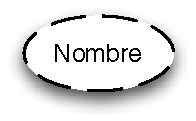
\includegraphics[scale=0.7]{colaboracion.pdf}
	\end{center}
	\caption{Representaci�n de una colaboraci�n.}
	\label{fig:colaboracion}
\end{figure}
\item {\bf ClassifierRole} (papel representado por el clasificador): es un rol espec�fico que juega un participante en una colaboraci�n. Especifica un {\em punto de vista restringido} de un clasificador, definido por lo que es requerido en la colaboraci�n.
\item {\bf Mensaje}: expresa una comunicaci�n entre instancias. Es una parte del patr�n de comunicaci�n representado por una interacci�n. La notaci�n utilizada para definir un mensaje es una flecha.
\item {\bf AssociationRole} (asociaci�n de un rol): una {\em association role} es un uso espec�fico de una asociaci�n necesaria en una colaboraci�n. Concreta un punto de vista limitado de una asociaci�n entre clasificadores.
\item {\bf Generalizaci�n}: es una relaci�n taxon�mica\footnote{Taxonom�a: Ciencia que trata de los principios, m�todos y fines de la clasificaci�n.} entre un elemento general y otro elemento m�s espec�fico. Se representa de esta manera:
\begin{figure}[H]
	\begin{center}
		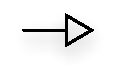
\includegraphics[scale=0.7]{generalizacion.pdf}
	\end{center}
	\caption{Representaci�n de una generalizaci�n.}
	\label{fig:generalizacion}
\end{figure}
\end{itemize}

A la hora de representar tanto los mensajes como los est�mulos existen diferentes tipos de flechas, las cuales describen diferentes tipos de flujo de control, entre �stas las m�s conocidas son:
\begin{figure}[H]
	\begin{center}
		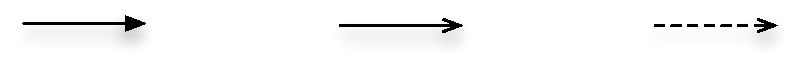
\includegraphics[scale=0.7]{arrows.pdf}
	\end{center}
	\caption{Tipos de flechas.}
	\label{fig:arrows}
\end{figure}

La primera flecha, empezando por la izquierda, representa una llamada a un procedimiento, aunque tambi�n puede ser utilizada para denotar que existen instancias activas y una de ellas env�a una se�al , esperando una secuencia de llamadas que complete el comportamiento antes de continuar, se distingue perfectamente porque tiene la punta rellena. La siguiente flecha denota una comunicaci�n as�ncrona, es decir, el emisor dispara el est�mulo e inmediatamente contin�a con el siguiente paso de la ejecuci�n.

Y por �ltimo la flecha discont�nua que refleja el hecho de regresar de la llamada a un procedimiento, como es l�gico estar� emparejada con una flecha del primer tipo, la flecha de retorno ser�a obviada cuando estemos al final de la activaci�n de un objeto.

Las {\bf etiquetas} que acompa�an a las {\bf flechas} que representan tanto los mensajes como los est�mulos tienen un formato determinado: \\
%\begin{center}
%\vspace*{1pt}
\hspace*{1cm}\verb!predecesor '/' guarda n�_de_secuencia valor ':=' nombre_msj argumentos!
%\end{center}

Para que veamos con un poco m�s de claridad los diferentes tipos de comunicaci�n que podemos tener utilizando este tipo de flechas vamos a representar unos diagramas de secuencia:

\begin{figure}[H]
	\begin{center}
		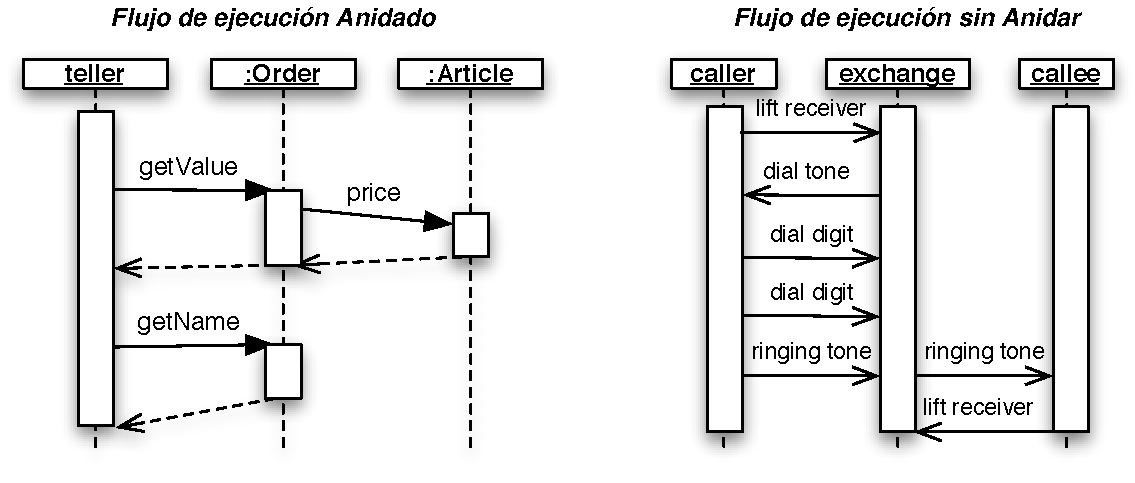
\includegraphics[scale=0.5]{communications.pdf}
	\end{center}
	\caption{Tipos de comunicaci�n.}
	\label{fig:communications}
\end{figure}

\subsection{Tricotom�a Clasificador-Instancia-Rol}
Una de las cosas que se puede hacer m�s complicado a la hora de la comprensi�n de los diagramas de interacci�n, en general, es diferenciar entre los conceptos de instancia, clasificador y papel que juega un clasificador dentro de la colaboraci�n, lo que denominamos {\em rol}.

Una {\bf instancia} es una entidad con comportamiento y un estado, y adem�s tiene un identidad �nica.
Un {\bf clasificador} es una descripci�n de una instancia.
Un {\bf rol del clasificador} define un uso (una abstracci�n) de una instancia.
La relaci�n existente entre estos elementos queda patente en la figura \ref{fig:trychotomy}.

\begin{figure}[H]
	\begin{center}
		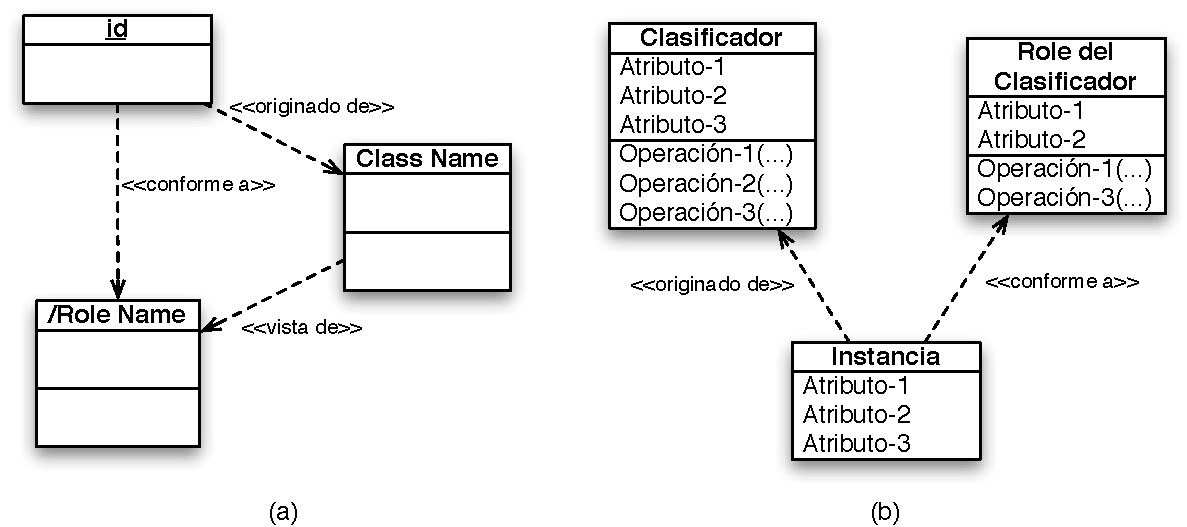
\includegraphics[scale=0.5]{trichotomy.pdf}
	\end{center}
	\caption{Tricotom�a Clasificador-Instancia-Rol.}
	\label{fig:trychotomy}
\end{figure}

Los atributos de una instancia corresponden a los atributos que posee su clasificador. Todos los atributos requeridos por el {\em rol del clasificador} tienen su atributo correspondiente en la instancia. Todas las operaciones definidas en el clasificador de la instancia pueden ser aplicadas a la instancia.
Todas las operaciones requeridas por el rol del clasificador, son aplicables a la instancia.

Otra situaci�n un tanto confusa que podemos encontrarnos es la diferencia existente entre la asociaci�n de un rol y la asociaci�n que relaciona los clasificadores, como se puede observar en el siguiente modelo existen sutiles diferencias entre ambas:

\begin{figure}[H]
	\begin{center}
		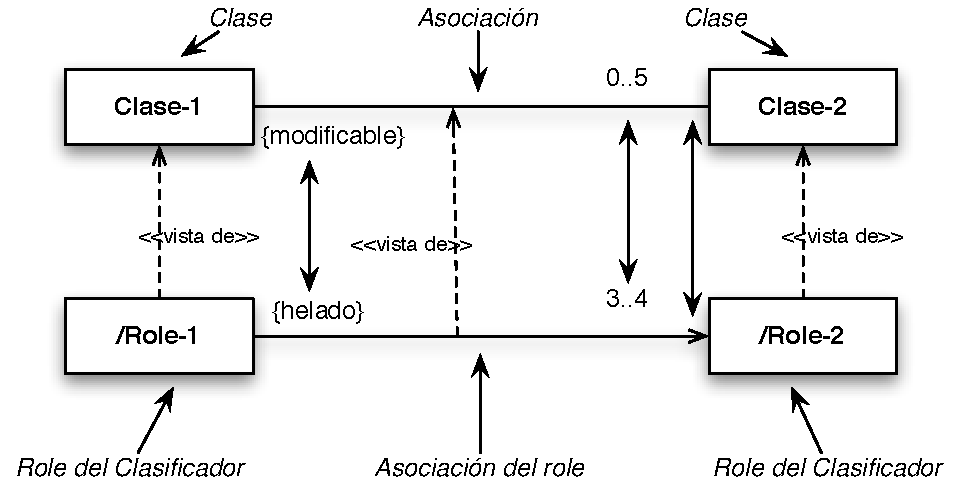
\includegraphics[scale=0.7]{associationRole.pdf}
	\end{center}
	\caption{Asociaci�n y asociaci�n de los roles.}
	\label{fig:associationRole}
\end{figure}

%\subsection{Tipos de colaboraci�n}
%Debemos diferenciar entre dos tipos de colaboraci�n: por un lado tenemos la colaboraci�n a nivel de %especificaci�n, lo que se conoce en la especificaci�n del lenguaje como {\em Collaboration}, y la %colaboraci�n a nivel de instancia, tambi�n denominada {\em CollaborationInstanceSet}.

%\subsubsection{Colaboraci�n a nivel de especificaci�n}
%Una colaboraci�n a nivel de especificaci�n puede estar asociada a un tipo, una operaci�n o a un %caso de uso. Este tipo de colaboraci�n estar� constitu�do por una serie de elementos que son los %clasificadores (ClassifierRoles), las asociaciones entre los clasificadores, denominadas %AssociationRole, interacciones y mensajes.

%\subsubsection{Colaboraci�n a nivel de instancia}
%Una colaboraci�n puede estar asociada a una clase, a un m�todo (implementaci�n de la operaci�n), %o a la realizaci�n de un caso de uso

	 \chapter{ArgoUML}
 \label{chap:argo}
 \section{Deficiencias de los diagramas de colaboraci�n}

Como hemos comentado con anterioridad ArgoUML es un programa de software libre, la mayor problem�tica existente con este tipo de proyectos es que la dedicaci�n que los desarrolladores invierten en ellos, est� muy determinada por su tiempo libre ya que, como norma general, estos productos no son implementados con �nimo de lucro, sino para cubrir una necesidad detectada por una cierta comunidad de usuarios, que ser�n los que a la postre lleven el peso de la implementaci�n.

Con todo esto es l�gico que algunos de estos proyectos manifiesten ciertas deficiencias en su implementaci�n, ArgoUML no es una excepci�n a todo esto, es m�s, las librer�as utilizadas por �ste tambi�n han sido desarrolladas de la misma forma, como consecuencia de ello presenta algunas carencias que nos afectaron a la hora de la realizaci�n de nuestro trabajo.

Todas estas deficiencias se engloban en varios grupos:
\begin{itemize}
\item {\bf Diagramas enteros sin implementar}: Como es el caso de los diagramas de secuencia, aunque seg�n queda reflejado en la p�gina de ArgoUML se espera que en la versi�n 0.20 vuelva a estar  soportado por la herramienta.
\item {\bf Elementos incorrectamente  implementados}: Normalmente esto se debe a una incorrecta interpretaci�n de las caracter�sticas descritas en la especificaci�n de UML.
\item {\bf Funcionalidades  poco desarrolladas}: �sto se ve reflejado, por ejemplo, en que la impresi�n de los diagramas no satisface grandes expectativas, lo mismo que ocurre con la generaci�n de c�digo y alg�n que otro fallo de programaci�n, como excepciones no capturadas debidamente.
\item {\bf Diagramas que no contemplan varios elementos} que se encuentran descritos en el est�ndar UML dentro de ellos, este �ltimo grupo ser� el que m�s nos afecte a la hora de poder realizar nuestro trabajo, en concreto, en el proceso de traducci�n.
\end{itemize}

Es importante tener en cuenta el hecho de que ArgoUML soporta en estos momentos la versi�n 1.3 de UML, esta versi�n ya qued� obsoleta a finales de 2003, este retraso en cuanto a la evoluci�n de UML es debido a la librer�a Java que proporciona a ArgoUML una implementaci�n del metamodelo de UML: la librer�a {\bf NSUML} \cite{NSUML}.

Esta librer�a implementa la versi�n de UML con la que trabaja Argo, se encuentra inacabada con diversos fallos y en un estado de abandono en su desarrollo por parte de la empresa que inici� este proyecto, la documentaci�n que proporcionan es muy deficiente lo que hace m�s complicado la actualizaci�n de dicha librer�a.

A continuaci�n pasaremos a citar las carencias detectadas a lo largo del desarrollo de nuestro proyecto, �stas est�n agrupadas en dos apartados que se�alaremos a continuaci�n:

\begin{itemize}
\item{\bf Elementos no implementados en el Diagrama de Colaboraci�n}:
	\begin{itemize}
	\item No es posible incluir un objeto m�ltiple (o multiobjeto) en uno de estos diagramas. Un {\bf multiobjeto} representa un conjunto de instancias de una determinada clase, es usado para mostrar que, ciertas operaciones y se�ales, van dirigidas a un conjunto, en vez de a una �nica instancia como ocurre habitualmente. Su representaci�n ser�a algo como esto:
	\begin{figure}[H]
		\begin{center}
			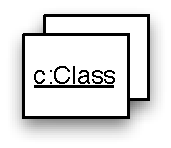
\includegraphics[scale=0.75]{multiobject.pdf}
		\end{center}
		\caption{Representaci�n gr�fica de un objeto m�ltiple.}
		\label{fig:multiobject}
	\end{figure}
	
	\item ArgoUML no permite a�adir un objeto activo dentro de una colaboraci�n. Un {\bf objeto activo} es aquel que posee el hilo de control e iniciar�a la actividad de control, dicho de otra forma, ser� el encargado de iniciar la colaboraci�n. Normalmente se suele representar del mismo modo que un objeto com�n, �nicamente que aparecer�a resaltado en negrita como puede observarse en la figura \ref{fig:activeObject}:
	\begin{figure}[H]
		\begin{center}
			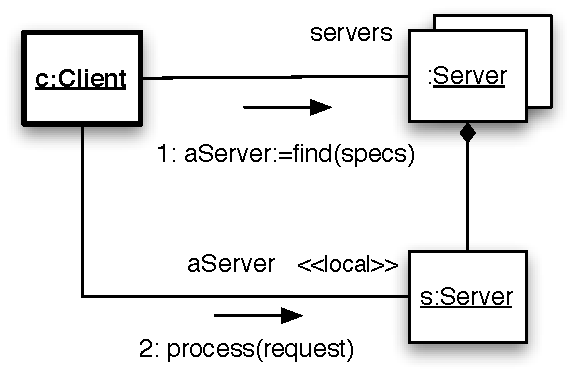
\includegraphics[scale=0.75]{activeObject.pdf}
		\end{center}
		\caption{Representaci�n gr�fica de un diagrama con un objeto activo.}
		\label{fig:activeObject}
	\end{figure}
	\item No podemos crear elementos a nivel de instancia, s�lo a nivel de especificaci�n. Esto impide que utilicemos instancias (en lugar de clasificadores), al igual que ocurre con los est�mulos (en vez de los mensajes), por supuesto tampoco se puede modelar enlaces entre objetos.
	\item La herramienta CASE no permite representar actores dentro de un diagrama de colaboraci�n, por lo tanto no podr�amos modelar un diagrama de este estilo:
	\begin{figure}[H]
		\begin{center}
			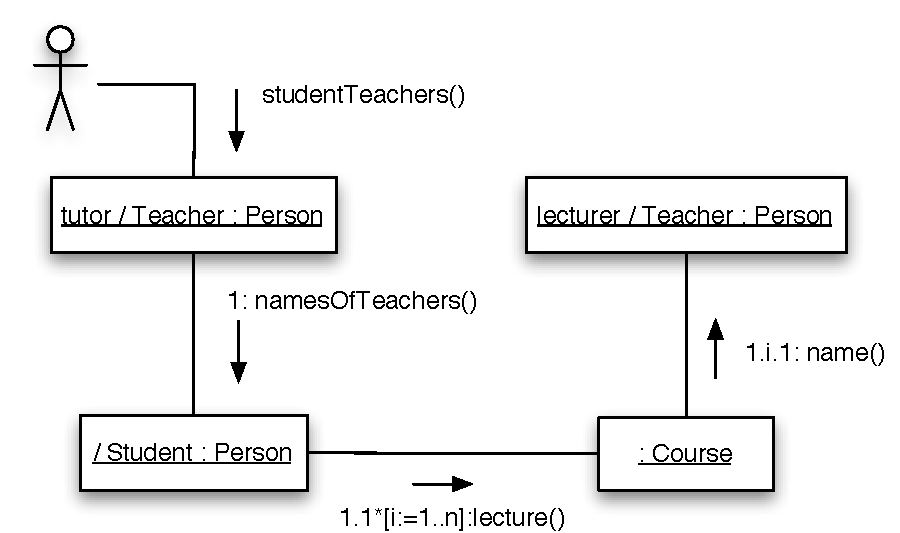
\includegraphics[scale=0.75]{actor.pdf}
		\end{center}
		\caption{Representaci�n gr�fica de un actor en un diagrama de colaboraci�n.}
		\label{fig:actor}
	\end{figure}
	\end{itemize}
	\item En ArgoUML no aparece el s�mbolo de la colaboraci�n (ver \ref{fig:colaboracion}), por lo que tendremos un menor n�mero de posibilidades de relacionar una colaboraci�n con otros elementos de nuestro modelo, como por ejemplo con clasificadores, con instancias o con casos de uso:
	
	\begin{figure}[H]
		\begin{center}
			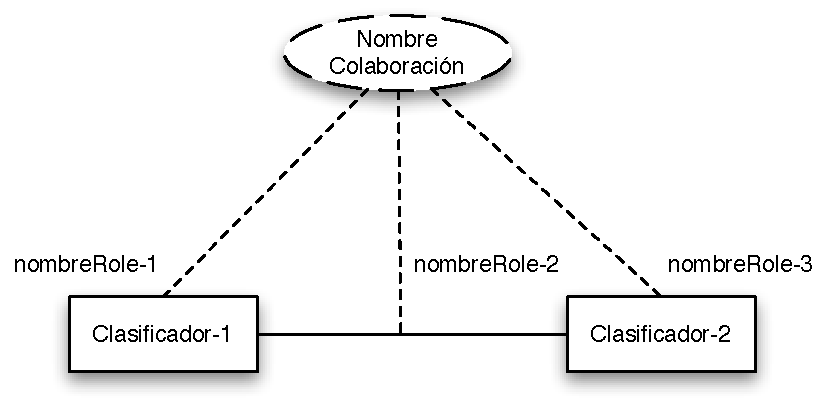
\includegraphics[scale=0.75]{collabDiag.pdf}
		\end{center}
		\caption{Diagrama que representa una colaboraci�n y sus clasificadores.}
		\label{fig:collabDiag}
	\end{figure}
	
	\item Es importante se�alar que la implementaci�n del diagrama de colaboraci�n de Argo no soporta la representaci�n de la {\bf ejecuci�n} de una acci�n {\bf condicionada} al cumplimiento de una situaci�n. Al igual que tampoco ofrece la posibilidad de expresar la {\bf ejecuci�n} de un mensaje de forma {\bf iterativa}. Estas dos carencias han hecho que no nos sea posible utilizar todas las notaciones que dispon�amos para este diagrama.
\item{\bf Elementos implementados que presentan deficiencias}:
	\begin{itemize}
	\item No se puede establecer una asociaci�n entre el papel representado por un clasificador y una clase existente dentro de nuestro modelo, es decir, no podemos reflejar la relaci�n clasificador y su rol.
	\item Los diagramas de colaboraci�n no pueden ser creados sin que est�n asociados a un caso de uso (m�s concretamente a un actor de un caso de uso) o a una clase (perteneciente a un diagrama de clases) que tengamos modelada en nuestro sistema previamente. Esta caracter�stica queda completamente fuera de la sem�ntica que aparece en la especificaci�n de UML, puesto que el diagrama de colaboraci�n se encarga de representar la interacci�n entre objetos de diferentes clases a trav�s de mensajes, no vemos que tenga sentido que para crearse estos diagramas tengan que estar asociados a alguna clase o a alg�n actor, por ejemplo en el esquema \ref{fig:actor}, �a qu� clase tendr�amos que asociar ese diagrama de colaboraci�n? A la clase {\em Person} o la clase {\em Course}. Seg�n la especificaci�n no tendr�amos porque tomar esta decisi�n ya que no se establece una relaci�n directa con ninguna de las dos clases, sino que el diagrama estar�a al mismo nivel que el diagrama de clases o que los casos de uso.
%	Tenemos que comentar que esta peculiaridad a complicado aunque s�lo sea ligeramente la %implementaci�n de nuestro traductor.
	\item ArgoUML no sigue estrictamente la notaci�n para representar los nombres de los clasificadores indicada por la especificaci�n del est�ndar, puesto que el clasificador tiene un formato claramente definido:
	\begin{center}
	\verb! "nombre_del_objeto" / "nombre_del_rol" : "nombre_de_la_clase"!
	\end{center}
	En nuestro caso no es posible escribir el nombre de la clase a la cual va asociada.
	\item Los mensajes no pueden cambiar su orientaci�n una vez han sido representados en una asociaci�n entre clasificadores. �nicamente contamos con un tipo de mensaje, los mensajes s�ncronos (comunicaci�n s�ncrona). El orden de los mensajes es generado autom�ticamente por la herramienta.
	\item Las acciones tambi�n muestran su falta de correcci�n en relaci�n a lo apuntado en la especificaci�n estudiada, �stas no pueden estar asociadas a los m�todos de una clase, ni tampoco podemos pasarle argumentos a una acci�n.
	\end{itemize}
\end{itemize}

Todas estas carencias nos llevan a la conclusi�n de que todav�a falta bastante trabajo para que los diagramas de colaboraci�n est�n implementados de acuerdo a toda la expresividad que ofrece UML, aunque tenemos que decir que son los �nicos representantes, por el momento, de los diagramas de interacci�n en la herramienta CASE que utilizamos.

\newpage

\section{XMI}
\label{sec:xmi}
Cuando la OMG public� en 1997 un {\bf RFP} (Request For Proposal) para un formato de intercambio de modelos basado en Stream \cite{SMIF}(Stream-Based Model Interchange Format -{\bf SMIF}) se presentaron Unisys, IBM, Oracle, y otras compa��as con la propuesta de {\bf XMI}.

Como su propio nombre indica XMI ({\bf X}ML {\bf M}etadata {\bf I}nterchange) es un formato de intercambio de {\bf metadatos} basado en {\bf XML}. Antes de continuar, consideramos necesario realizar unos comentarios acerca de XML.

XML \cite{XML} significa e{\bf X}tensible {\bf M}arkup {\bf L}anguage, es un subconjunto de {\bf SGML} ({\bf S}tandard {\bf G}eneralized {\bf M}arkup {\bf L}anguage), la funcionalidad que convierte a XML en una herramienta tan poderosa es que es un {\bf metalenguaje}, es decir, que es un lenguaje utilizado para definir otros lenguajes de marcado que se adec�en a un problema concreto.

Adem�s de esta caracter�stica tambi�n podemos mencionar el hecho de que es un est�ndar del W3C \cite{W3C}, en su contenido (determinado por un {\bf DTD} \cite{DTD} o Definici�n del Tipo de Documentos) se combina tanto los datos como los metadatos para el intercambio de informaci�n, es flexible e independiente del sistema y las etiquetas forman una estructura en �rbol ({\bf DOM} \cite{DOM} Modelo de Objetos del Documento). En la figura \ref{fig:xml} est�n representados todos los elementos que hemos mencionado.

\begin{figure}[H]
	\begin{center}
		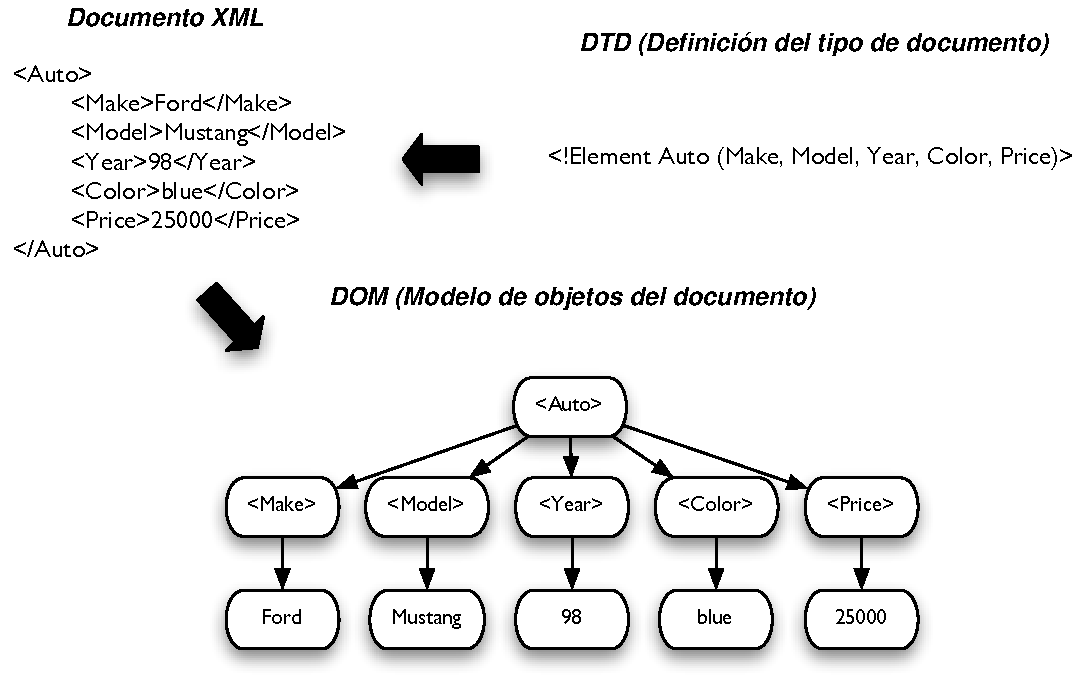
\includegraphics[scale=0.7]{xml.pdf}
	\end{center}
	\caption{Relaci�n entre XML, DTD y DOM.}
	\label{fig:xml}
\end{figure}

El objetivo �ltimo de la definici�n de un formato como XMI era la integraci�n de herramientas aplicaciones y repositorios que trabajaban con metamodelos que eran conformes a {\bf MOF} ({\bf M}odel {\bf O}bject {\bf F}acility).

\subsection{MOF}
UML es un est�ndar utilizado para describir {\em modelos de objetos}. Desde un punto de vista arquitect�nico el modelo de UML est� estructurado en tres niveles: 
\begin{itemize}
\item {\bf Metamodelo}: El metamodelo de UML define un n�mero de elementos tales como {\em Class}, {\em Operation}, {\em Attribute}, {\em Association}, y algunos m�s. Estos elementos se llaman {\bf metaclases}.
\item {\bf Modelo}: Instancias de una {\em Class} de UML representan entidades, y procesos. Por ejemplo: 

\begin{figure}[H]
	\begin{center}
		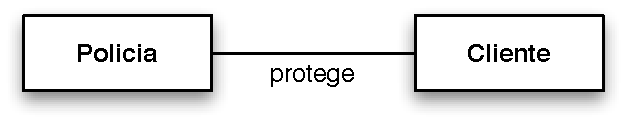
\includegraphics[scale=0.7]{clases.pdf}
	\end{center}
	\caption{Clase Policia y Cliente.}
	\label{fig:clases}
\end{figure}

Se puede definir tambi�n instancias de la metaclase Association entre clases, tal como la asociaci�n ({\em protege} ver \ref{fig:clases}) entre Cliente y Policia. Estas instancias de metaclases de UML se denominan {\bf metaobjetos}.

\item {\bf Objetos del usuario}: Son instancias de los elementos del modelo. Por ejemplo instancias de la clase {\em Cliente} son: c123:Cliente, c456:Cliente. Estos son los objetos. Los modelos de objetos de UML de dominios particulares, se denominan {\em modelos de objetos de dominio} o {\em modelos de dominio}. 
\end{itemize}

Existen tambi�n otros metamodelos como son los metamodelos para sistemas de bases de datos. Un metamodelo de una base de datos define elementos b�sicos como base de datos, tabla, columna, clave, y dem�s. Que son usados para definir modelos de datos espec�ficos.

Tantos los modelos de objetos de dominio como los modelos de datos son guardados en bases de datos especializadas llamadas {\bf repositorios de metadatos}, algunas veces llamado simplemente como {\bf repositorio}. Los administradores de los repositorios normalmente necesitan manejar modelos de dominios y modelos de datos de una forma unificada, pero la naturaleza tan dispar de los metamodelos sobre los cuales est�n basados constituye un gran obst�culo. 

MOF provee una base com�n para esos metamodelos. Si dos metamodelos diferentes est�n de acuerdo con MOF, los modelos basados en ellos pueden residir en el mismo repositorio o intercambiarse por diferentes herramientas compatibles con �l. 

El metamodelo de UML est� basado en el est�ndar MOF, (es decir que sus constructores est�n definidos en t�rminos de los elementos {\em core} de MOF), y esto es una pieza clave de la estrategia de la OMG para soportar repositorios integrados. MOF define un conjunto de constructores que pueden ser usados para describir metamodelos. 

MOF agrega un cuarto nivel a la clasificaci�n que mostramos antes. MOF llama a estos niveles: M0, M1, M2, y M3.
\begin{itemize}
\item {\bf M3} (MOF core): Define los elementos usados para especificar metamodelos, como por ejemplo MetaClass, MetaAttribute, MetaAssociation, Mof::Class, Mof::Association, Mof::Attribute.
\item {\bf M2} (Meta-Model): Un metamodelo definido en t�rminos de los elementos core de MOF consiste de MetaClasses, MetaAttributes, y algunos otros. Como muestra, UML: Class, Attribute, Operation. Data Warehousing: Base de datos, tabla, fila.
\item {\bf M1} (Modelo): Un modelo expresado en t�rminos de un metamodelo. Modela un dominio de informaci�n espec�fico. Consiste de instancias de elementos de un metamodelo (es decir metaobjetos).
\item {\bf M0} (Objetos de usuario): Instancias de los elementos de un modelo.
\end{itemize}

XMI proporciona un mecanismo para derivar un XML-DTD que representa los constructores de un metamodelo compatible con MOF.

Una herramienta compatible con MOF puede por lo tanto representar y enviar un modelo de dominio basado en UML en la forma de XML cuya estructura est� de acuerdo a un XMl DTD. El objetivo de quienes env�an un XMI es que el XML sea usado para importar y exportar modelos desde y a un repositorio persistente.

Todo lo anterior justifica la sugerencia que realiza OMG en la definici�n de arquitectura propu
 en el profile \cite{UML-SPT}, de la utilizaci�n de XMI como formato de intercambio entre las diversas partes, como el editor y el configurador del modelo.

Despu�s de habernos puesto en situaci�n y teniendo claras las ideas que se han comentado pasamos a representar gr�ficamente, c�mo ArgoUML exporta los elementos m�s importantes (desde el punto de vista de nuestro trabajo) que podemos encontrarnos dentro de un modelo UML.

Lo primero que nos vamos a encontrar dentro de un fichero XMI generado con ArgoUML (0.18.1) es la siguiente cabecera:

\begin{figure}[H]
	\begin{center}
		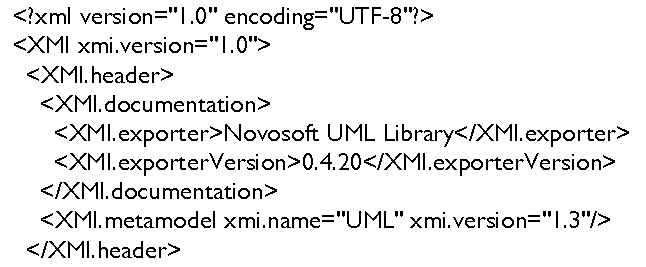
\includegraphics[scale=0.77]{xmiHeader.pdf}
	\end{center}
	\caption{Cabecera del documento XMI.}
	\label{fig:xmiHeader}
\end{figure}

La primera tambi�n conocida como {\em declaraci�n XML}, define la versi�n de XML que estamos utilizando, adem�s en nuestro caso tambi�n especificamos la codificaci�n del documento, en nuestro caso UTF-8. Despu�s de esta l�nea comienza informaci�n referente a la versi�n de XMI, cual es el metamodelo que mapea y su versi�n, UML v1.3 para nosotros, la l�nea que nos informa de esto es:
\verb!<XMI.metamodel xmi.name="UML" xmi.version="1.3"/>!.

Diremos que \verb!XMI.metamodel! es el {\bf elemento} de la etiqueta, \verb!xmi.name! ser� un {\bf atributo} del elemento anterior, lo mismo que xmi.version, y tanto \verb!"UML"! como \verb!"1.3"! ser�n los respectivos valores de los atributos. Un elemento podr� llevar anidados otros elementos, atributos o ambos. A continuaci�n vamos mostrar c�mo est�n serializados los diagramas en formato XMI.

\subsection{Diagrama de clases}

\begin{figure}[H]
	\begin{center}
		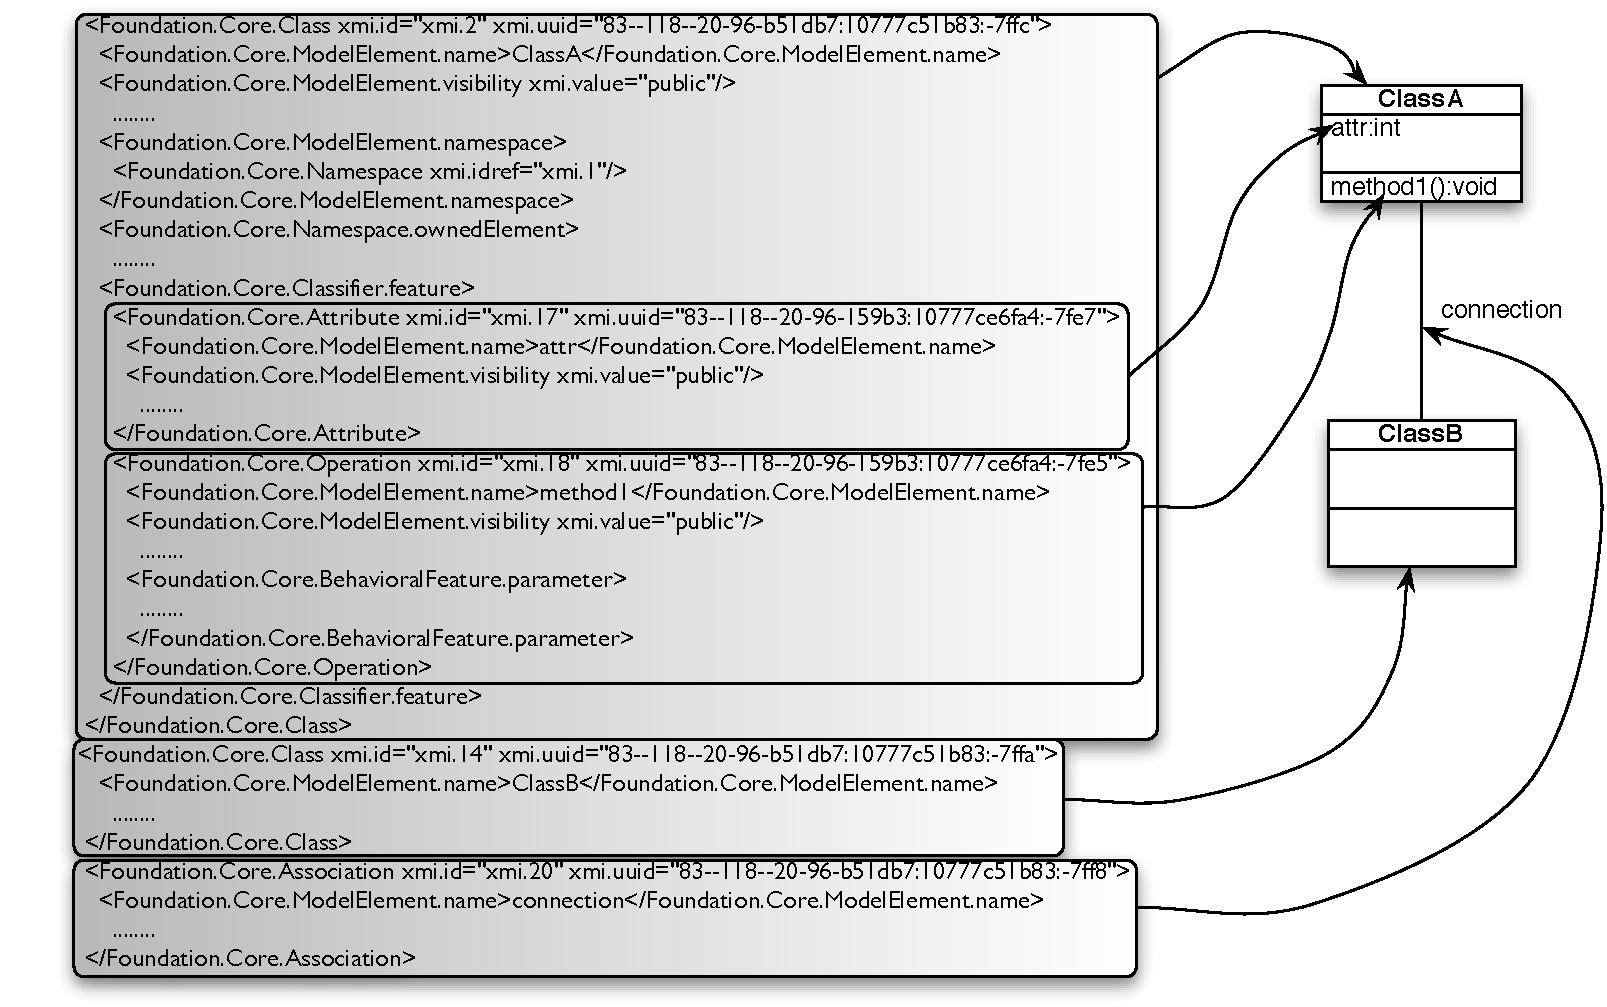
\includegraphics[scale=0.75,angle=90]{xmiClass.pdf}
		%\includegraphics[scale=0.75,angle=-90]{xmiClass.pdf}
	\end{center}
	\caption{Representaci�n XMI de los elementos del diagrama de clases.}
	\label{fig:xmiClass}
\end{figure}

\subsection{Diagrama de despliegue}

\begin{figure}[H]
	\begin{center}
		\includegraphics[scale=0.75,angle=90]{xmiDeploy.pdf}
		%\includegraphics[scale=0.75,angle=-90]{xmiDeploy.pdf}
	\end{center}
	\caption{Representaci�n XMI de los elementos del diagrama de desarrollo.}
	\label{fig:xmiDeploy}
\end{figure}

\subsection{Diagrama de estados}

\begin{figure}[H]
	\begin{center}
		\includegraphics[scale=0.75,angle=90]{xmiSM.pdf}
		%\includegraphics[scale=0.75,angle=-90]{xmiSM.pdf}
	\end{center}
	\caption{Representaci�n XMI de los elementos del diagrama de estados.}
	\label{fig:xmiSM}
\end{figure}

\subsection{Diagrama de colaboraci�n}

\begin{figure}[H]
	\begin{center}
		\includegraphics[scale=0.75,angle=90]{xmiCollab.pdf}
		%\includegraphics[scale=0.75,angle=-90]{xmiCollab.pdf}
	\end{center}
	\caption{Representaci�n XMI de los elementos del diagrama de colaboraci�n.}
	\label{fig:xmiCollab}
\end{figure}
	%\input{deficiency.tex}

	\chapter{Implementaci�n de soluciones}
\label{chap:impl}

A lo largo de este anexo vamos a exponer los detalles m�s importantes de la implementaci�n de ArgoSPE que han estado directamente relacionados con mi proyecto, los cuales fueron estudiados para poder extender adecuadamente la herramienta, sin provocar ninguna modificaci�n no deseada dentro del comportamiento de la aplicaci�n.

En este ap�ndice comentaremos los fallos m�s relevantes que hemos encontrado, fundamentalmente en el proceso de traducci�n de m�quinas de estados a LGSPN's. Para finalizar dejaremos constancia de c�al ha sido el resultado final tanto de los procesos de traducci�n de los diagramas de colaboraci�n, como del mecanismo de composici�n con las LGSPN's de las m�quinas de estado.

\section{Errores}

%Como ya se ha mencionado con anterioridad nuestro trabajo est� fuertemente ligado al proceso de %traducci�n de las m�quinas de estado.
\subsection{Modificaci�n caso A}
\begin{figure}[H]
	\begin{center}
		\includegraphics[scale=0.75]{casoAB.pdf}
	\end{center}
	\caption{Representaci�n de la traducci�n original del estado N.}
	\label{fig:casoAB}
\end{figure}

La figura anterior \ref{fig:casoAB} muestra la traducci�n propuesta en \cite{Merse-PhD} para un estado que posee una {\em do/activity}\footnote{Acci�n que deber� realizar un objeto de esa clase cuando permanezca en el estado representado en el esquema.}, un evento diferido y una transici�n interna\footnote{La diferencia entre una transici�n interna y una autotransici�n es que cuando se produce una transici�n interna no se ejecuta ni la acci�n de entrada ni la acci�n de salida.}.

En el trabajo \cite{PFC-Borja} su autor consider� oportuno realizar una serie de modificaciones con el fin de evitar la duplicidad de etiquetas que se produc�an con la transformaci�n anterior, por ejemplo, en las transiciones que representan la transici�n interna del estado, etiquetadas con \verb!| int!. Como resultado de estas transformaciones la red de Petri resultante del estado mencionado anteriormente quedar�a algo como esto:

\begin{figure}[H]
	\begin{center}
		\includegraphics[scale=0.7]{modifiedCaseA.pdf}
	\end{center}
	\caption{Representaci�n de la traducci�n modificada del estado N.}
	\label{fig:modifCasoA}
\end{figure}

Se puede apreciar claramente en la figura que uno de los arcos dirigidos que hemos representado, tiene un color diferente del resto de los elementos que constituyen el esquema, en este caso el {\bf azul}, gracias a las revisiones realizadas de nuestro m�dulo se advirti� la ausencia de esa transici�n que implicaba una modificaci�n en el comportamiento que deb�a modelar la RdP.

Tambi�n cabe destacar el hecho de la aparici�n de un {\em estado} al que hemos denominado {\em Basura}, la representaci�n de este estado en elementos del dominio de las RdP viene reflejada en la parte derecha, la figura {\em b}, el lugar Basura recibe las marcas que representan los objetos que han terminado la ejecuci�n de la acci�n del estado y que deben ser eliminados de la red para conseguir un funcionamiento correcto de la misma, ya que sino podr�a impedirse el disparo de la transici�n temporizada que describe la acci�n del estado.

En el esquema \ref{fig:modifCasoA} podemos comprobar que existen dos arcos con un c�rculo en uno de los extremos, estos arcos se denominan {\bf arcos inhibidores}, estos arcos hacen que la transici�n que los contiene {\bf no} pueda dispararse si en el lugar enlazado por cada uno de los arcos existen al menos tantas marcas como indica el peso del arco. Estos arcos son una extensi�n de las RdP para implementar la l�gica negativa.

Despu�s de presentar la modificaci�n hemos considerado adecuado explicar brevemente el comportamiento din�mico modelado por la RdP para que el lector se pueda hacer una idea m�s clara de los pasos que realiza una instancia cuando se encuentra en un estado, vamos a representar este recorrido a trav�s de la figura \ref{fig:exeCasoA}.

\begin{figure}[H]
	\begin{center}
		\includegraphics[scale=0.7]{executionCaseA.pdf}
	\end{center}
	\caption{Ejecuci�n de la red de Petri modificada del estado N.}
	\label{fig:exeCasoA}
\end{figure}

Lo primero que tenemos que comentar es que se ha comprobado que el comportamiento descrito por la  RdP original y la modificada es el mismo, por lo que no perdemos nada de sem�ntica con la transformaci�n, as� que consideraremos la modificaci�n como {\bf correcta}.

Dicho esto es preciso aclarar la existencia de dos nubes en cada una de las RdP que componen el esquema, la primera indica que esas RdP son parte de la RdP que representa la m�quina de estados en la que se encuentra el estado N, pero que no hemos querido reflejar para evitar la complejidad que supone la representaci�n de la RdP completa del diagrama de estados.

La otra nube tiene un prop�sito similar aunque esta vez, intentamos reflejar que existen otros elementos pertenecientes a esa red que modelan tanto, la transici�n interna, como la transici�n de salida del estado, como el evento diferido.

La figura \ref{fig:exeCasoA} 1), representa la situaci�n en la que una instancia de la clase representada por la m�quina de estados en la que se encuentra el estado N, ha entrado en ese estado. Lo primero que tiene que hacer nada m�s entrar ser� ejecutar la acci�n de entrada ({\em entry action}) asociada al estado, como nos podemos imaginar si nos fijamos en las etiquetas la {\em entry action} est� modelada como una transici�n inmediata.

La ejecuci�n de esta acci�n es recogida en la red de Petri con el disparo de la transici�n etiquetada como \verb!| entry!, se puede observar que se cumplen todos los requisitos para el disparo de la misma, ya que todos los lugares de entrada, en este caso el etiquetado con \verb!| ini_N!, tienen como m�nimo el n�mero de marcas que indica el peso del arco que lo enlaza con la transici�n, es decir, uno.

Como resultado del disparo de la transici�n (o ejecuci�n de la acci�n de entrada), la marca pasa a  estar situada en su lugar de salida, \verb!| end_entry_N!, (ver \ref{fig:exeCasoA} figura 2)). Si nos fijamos con atenci�n vemos que la transici�n temporizada tiene {\bf dos} lugares de entrada, el lugar de la salida de la transici�n anterior y el lugar \verb!| compl_N!, el primero contiene una marca, pero el segundo no contiene ninguna aunque esto es exactamente lo que necesitamos para que la transici�n se encuentre sensibilizada, ya que este lugar lo enlaza un arco inhibidor a la transici�n.

Por tanto el disparo de la transici�n se efectuar� una vez se haya producido el retraso indicado por la anotaci�n asociada a dicho estado dentro del modelo UML. El resultado de este disparo hace que el marcado de la red sea el presentado en la figura 3 del esquema \ref{fig:exeCasoA}.

En este momento vemos que ha aparecido una marca en el lugar \verb!| compl_N! y otra en \verb!| end_entry_N!, lo cual produce que {\bf ninguna} de las transiciones de la RdP, que estamos contemplando, est� sensibilizada, esto es debido a la acci�n de los arcos inhibidores.

La �nica manera que tenemos para que la red modifique su marcado ser� que se produzcan algunas de las opciones que han sido encerradas en la nube, es decir, que se produzca el evento que dispare o la transici�n interna, o la de salida, o bien sea un evento diferido. 

Vamos a suponer que el evento que dispara la transici�n de salida ha sido generado desde el exterior de la m�quina de estados, esto har� que la marca del lugar \verb!| end_entry_N! desaparezca y se dispare la transici�n que introduzca la marca de \verb!| compl_N! dentro del estado Basura. Con lo que obtendremos el marcado expuesto en la figura \ref{fig:exeCasoA} 4), de esta manera la red queda lista para otra instancia de la clase.

\subsection{Traducci�n del pseudoestado elecci�n}

Al comienzo de nuestro proyecto fueron notificadas dos situaciones que podr�an producir un error en la traducci�n, la primera ha sido comentada en la subsecci�n anterior y la segunda se refiere a la traducci�n que se realizaba de los pseudoestados elecci�n (o {\em choice pseudostates}), elementos pertenecientes a las m�quinas de estados.

Los {\bf pseudoestados de elecci�n} resultan de la evaluaci�n din�mica de las guardas de  sus transiciones de salida, por lo cual definen una ramificaci�n condicional din�mica. Esto significa que la  transici�n de salida a tomar depende de una funci�n o resultado previamente calculado. Las guardas tienen un valor booleano, son exclusivas y al menos una de ellas debe devolver el valor cierto para que el modelo est� bien formado.

Una de las cosas m�s importantes para poder analizar si la traducci�n a RdP es correcta es comprender qu� se est� modelando desde el nivel de UML, para ello vamos a ver un sencillo ejemplo para explicar el significado de lo que modelamos.

\begin{figure}[H]
	\begin{center}
		\includegraphics[scale=0.65]{choice.pdf}
	\end{center}
	\caption{Diagrama de estados con un pseudoestado choice.}
	\label{fig:choice}
\end{figure}

\begin{figure}[H]
	\begin{center}
		\includegraphics[scale=0.7]{translationChoice.pdf}
	\end{center}
	\caption{Traducci�n del diagrama de estados de la figura \ref{fig:choice}.}
	\label{fig:translationChoice}
\end{figure}

Podemos obsevar en la figura \ref{fig:choice} que es una de las m�quinas de estados m�s simple que se puede modelar conteniendo un pseudoestado de elecci�n. Cuando sea recogido un evento de tipo {\em ev1} por esta m�quina de estados la transici�n de salida del {\em estado A} ser� disparada, entonces entraremos en el pseudoestado de elecci�n, para representar la verificaci�n de una guarda hemos colocado unas anotaciones en cada una de las transiciones de salida de la elecci�n, esto indica la probabilidad con la que nos decantaremos por una de las transiciones de salida del {\em branch}, nombre por el que tambi�n es conocido el estado de elecci�n.

Al utilizar este pseudo estado hemos variado el comportamiento normal de las transiciones de las m�quinas de estados, puesto que ahora al dispararse la transici�n de salida no ejecutaremos la acci�n que hemos modelado como efecto de la misma, sino que se ejecutar� el efecto (o acci�n) de la rama que se escoja en el {\em choice}. 

Los eventos desencadenantes de las transiciones de salida del {\em branch}, tambi�n son inocuos debido a que una instancia no permanecer� en el pseudoestado elecci�n como podr�a hacerlo en un estado normal, por lo que el �nico evento que se tendr� en cuenta a la hora de cambiar de estado es el modelado en la transici�n de salida de {\em A}.

%La traducci�n realizada por ArgoSPE para la m�quina de estados est� representada en la figura %\ref{fig:choice} ser� la siguiente:

Debemos comentar que la RdP representada en la figura \ref{fig:translationChoice} no es exactamente id�ntica a la que aparece en la traducci�n de nuestra aplicaci�n, ya que faltan algunas partes como la traducci�n de los estados {\em B} y {\em C}, pero en lo referente al pseudoestado de elecci�n, que hemos denominado {\em choice}, es su representaci�n {\bf exacta}. 

Como apreciamos en la figura \ref{fig:translationChoice} la LGSPN resultante representa perfectamente lo que quer�amos modelar con la m�quina de estados inicial, con lo cual tenemos que concluir que la traducci�n realizada por nuestra aplicaci�n es la adecuada.

\newpage

\section{Traducci�n}

Este es uno de los puntos m�s importantes de nuestro trabajo, debido a que es la base de una correcta composici�n con las m�quinas de estado, y guarda adem�s una estrecha relaci�n con la consulta que hemos implementado.

Antes de comenzar con la traducci�n de los diagramas de colaboraci�n debemos dejar constancia de la representaci�n de los diagramas de estados en el dominio de las GSPN's.
 
\subsection{M�quinas de estado}

Cada m�quina de estados que compone el modelo UML que hemos dise�ado ser� representada por una �nica RdP, el proceso de obtenci�n de esta red est� basado en la composici�n de peque�as subredes que son obtenidas tanto de la traducci�n de los estados que componen la m�quina como de las transiciones que unen a dichos estados.

La subred generada de la traducci�n de un estado UML depender� de los elementos que presente dicho estado, como por ejemplo, la existencia de una {\em entry action}, de una {\em do activity} o de transiciones internas pueden hacer variar de una manera significativa la red obtenida.

Lo mismo ocurre en el caso de las transiciones, aunque esta vez tendremos que fijarnos en si la transici�n cuenta con un disparador ({\em trigger}) y un efecto ({\em effect}). Estos dos elementos son los que utilizaremos como puntos de conexi�n con otros elementos del modelo.

Para nuestro trabajo ha resultado muy pr�ctico conocer al detalle la implementaci�n de c�mo estaban traducidos los diagramas de estados dentro de la herramienta, en primer lugar para poder reparar los defectos que hab�an sido encontrados y posteriormente para realizar unas cuantas modificaciones, que nos facilitar�an m�s tarde la tarea de la composici�n.

Lo anteriormente dicho pone de manifiesto la importancia de conocer al detalle la traducci�n de este tipo de diagramas, motivo por el cual intentaremos dar la mayor precisi�n posible a esta secci�n. Para ello creemos necesario modelar una m�quina de estados con la gran parte de los elementos que podemos encontrar en ella, para posteriormente ir asociando estos elementos con su traducci�n. El modelo de UML utilizado ser�:

\begin{figure}[H]
	\begin{center}
		\includegraphics[scale=0.7]{classModelSM.pdf}
	\end{center}
	\caption{Diagrama de Clases a traducir.}
	\label{fig:classModelSM}
\end{figure}

\begin{figure}[H]
	\begin{center}
		\includegraphics[scale=0.7]{modelSM.pdf}
	\end{center}
	\caption{M�quina de estados a traducir.}
	\label{fig:modeloSM}
\end{figure}

Con el fin de representar lo m�s claramente posible la RdP resultante de la traducci�n del diagrama de estados vamos a representar por separado cada una de las RdP de cada estado.

%	\begin{flushleft}
%	\end{flushleft}
\begin{figure}[H]
	\begin{center}
		\includegraphics[scale=0.63]{translationInicio.pdf}
	\end{center}
	\caption{GSPN obtenida del estado inicio.}
	\label{fig:translationInicio}
\end{figure}

En esta primera red \ref{fig:translationInicio} queda representado como es traducido el estado {\em inicio} en el que �nicamente contamos con un elemento relevante, la transici�n de salida, esta transici�n posee un evento disparador y un efecto, la parte {\bf verde} de la red representa los elementos de la RdP asociados a la transici�n de salida, y los elementos de color {\bf naranja} ser�n los de la acci�n de entrada. 

En la siguiente red tambi�n hemos utilizado otros colores con el fin de distinguir qu� partes est�n relacionadas con ciertos elementos de UML, como por ejemplo el {\bf morado} con la {\em do activity} y el {\bf azul} con la transici�n interna.

Tambi�n podemos encontrar elementos en un color {\bf negro}, estos elementos no est�n relacionados con  ning�n componente concreto de UML sino que forman parte de la RdP, por ejemplo, los lugares cuyas etiquetas empiezan por \verb!| e_!, o \verb!| ack_!, son lugares de enlace con otras m�quinas de estado. Cabe destacar la etiqueta \verb!lambda! que ser� utilizada cuando no exista el elemento que representa el lugar o la transici�n en la cual se coloque.

\begin{figure}[H]
	\begin{center}
		\includegraphics[scale=0.7]{translationMedio.pdf}
	\end{center}
	\caption{GSPN resultante del estado medio.}
	\label{fig:translationMedio}
\end{figure}

Se puede apreciar claramente c�mo dependiendo de los elementos que aparecen en UML la RdP cambia sustancialmente, este hecho queda reflejado en las diferencias entre la traducci�n del estado {\em inicio} y la del estado {\em medio}, este �ltimo posee acci�n de entrada, {\em do/activity}, transici�n de salida y transici�n interna, se puede decir que modela pr�cticamente todos los elementos que puede albergar un estado.  

\begin{figure}[H]
	\begin{center}
		\includegraphics[scale=0.7]{translationFin.pdf}
	\end{center}
	\caption{GSPN representante del estado fin.}
	\label{fig:translationFin}
\end{figure}

A simple vista vemos que la RdP del pseudoestado final de la m�quina de estados es la m�s sencilla de todas las que hemos presentado, esto se debe a la propia naturaleza de este elemento que simplemente expresa el fin de la vida de la instancia, su �ltimo lugar el etiquetado con \verb!| p_elements_class_ClassA! posee tantas marcas como poblaci�n tenga la clase cuya m�quina de estados estamos contemplando.

%\newpage

\subsection{Diagramas de colaboraci�n}

En algunas secciones anteriores de este documento (ver \ref{subsec:traduccion}) hemos mostrado con alg�n ejemplo simple c�mo se traduc�an los diagramas de colaboraci�n al dominio de las GSPN's. En esta secci�n queremos mostrar los cuatro tipo de traducciones posibles que podemos encontrar para los mensajes que ser�amos capaces de modelar en un diagrama de colaboraci�n de ArgoUML.

\begin{figure}[H]
	\begin{center}
		\includegraphics[scale=0.7]{translationMsjs.pdf}
	\end{center}
	\caption{GSPN's representantes de todos los tipos de mensajes.}
	\label{fig:translationMsjs}
\end{figure}

Tenemos que puntualizar una serie de detalles sobre esta traducci�n, la estructura de las RdP est� seguida exactamente como queda representada en la figura \ref{fig:translationMsjs}, aunque existen unas peque�as variaciones en cuanto a dos etiquetas de dos lugares.

Cuando estamos traduciendo el primer mensaje de una interacci�n el primer lugar de �ste tambi�n ser� el primer lugar del diagrama de colaboraci�n con lo que la etiqueta de este ser� \verb!| startCoD!, y no \verb!| _msj! como cabr�a esperar, lo mismo ocurre cuando estamos traduciendo el �ltimo mensaje de la interacci�n reflejada en el diagrama de colaboraci�n, su �ltimo lugar tambi�n ser� el �ltimo lugar del diagrama de colaboraci�n por lo que quedar� etiquetado como \verb!| endCoD!. 

Para que la traducci�n de un diagrama de colaboraci�n puede llevarse a cabo se tienen que cumplir una serie de condiciones en el modelo que queremos analizar, la primera de ellas indica que cada una de las clases que participa en la interacci�n descrita por el diagrama de colaboraci�n deber� describir su comportamiento por medio de un diagrama de estados. La segunda es referente a los mensajes y expresa que todos los mensajes que est�n recogidos dentro de un diagrama de colaboraci�n, tienen en la m�quina de estados del emisor una acci�n que causa el env�o del mismo, y en el diagrama de estados del receptor existir� al menos una transici�n que modele la respuesta a ese evento.

Esta segunda hip�tesis hace que debamos modificar el algoritmo de traducci�n que utilizaba la herramienta ArgoSPE antes de soportar la traducci�n de los diagramas de secuencia, est� claro que tenemos que poseer toda la informaci�n de todas m�quinas de estados que existen en el modelo para poder asegurar el cumplimiento de la segunda hip�tesis, de otra manera ser�a imposible.

Para representar el algoritmo de traducci�n antiguo y el modificado vamos a utilizar unos diagramas de actividades:

\begin{figure}[H]
	\begin{center}
		\includegraphics[scale=0.7]{algTraduccion.pdf}
	\end{center}
	\caption{Diagramas de actividades de los algoritmos de traducci�n de ArgoSPE.}
	\label{fig:algTraduccion}
\end{figure}

Como es evidente el algoritmo antiguo ser� el representado por el diagrama de actividades de la parte izquierda y el m�s reciente estar� reflejado en la parte derecha de la figura. Vemos que simplemente hemos tenido que sacar del bucle principal el recorrido de los diagramas de colaboraci�n que poseen cada una de las clases que constituyen el modelo.

\section{Composici�n}

El proceso de composici�n envuelve a la RdP resultante de la composici�n de las RdP de las m�quinas de estados y de los diagramas de actividad, con la RdP de uno de los diagramas de colaboraci�n que han sido modelados por el dise�ador del sistema software.

Esto quiere decir que realmente se tienen que realizar dos composiciones para poder conseguir la representaci�n, en el dominio de las RdP, de la situaci�n descrita por el diagrama de colaboraci�n seleccionado del sistema.

Lo l�gico ser� pues comenzar por representar c�mo se realiza la primera de las composiciones, principalmente nos interesar� conocer c�mo se fusionan las m�quinas de estados para poder obtener una representaci�n del sistema completo.

\begin{figure}[H]
	\begin{center}
		\includegraphics[scale=0.7]{mergeSM.pdf}
	\end{center}
	\caption{Esquema de la composici�n de dos m�quinas de estados.}
	\label{fig:mergeSM}
\end{figure}

Al observar con un poco de detenimiento la figura \ref{fig:mergeSM} vemos representado en la RdP c�mo, la clase {\em Emisor} ha modelado en la transici�n de salida inmediata del estado {\em iniS} el lanzamiento de un evento que ser� recogido por la m�quina de estados de la clase {\em Receptor}. 

Dicho de otra manera en la m�quina de estados de la clase Emisor existe una transici�n que tiene como efecto la ejecuci�n de la operaci�n \verb!Receptor.getConnection!, m�todo de la clase {\em Receptor}, que generar� un evento que podr� ser recibido por la m�quina de estados para que �sta modifique su estado. Esto produce que exista el efecto \verb!Receptor.getConnection! en la transici�n de salida del estado {\em iniS} y que a su vez tengamos un evento disparador en la transici�n de salida del estado {\em iniR}.

Una vez explicada de forma breve la composici�n entre m�quinas de estado vamos a suponer que tenemos un diagrama de colaboraci�n como este:

\begin{figure}[H]
	\begin{center}
		\includegraphics[scale=0.6]{simpleColaboracion.pdf}
	\end{center}
	\caption{Diagrama de colaboraci�n con un mensaje.}
	\label{fig:simpleColaboracion}
\end{figure}

Para poder observar m�s claramente la composici�n entre las RdP de las m�quinas de estados y la del diagrama de colaboraci�n hemos optado por un diagrama con un solo mensaje, ya que si se entiende el mecanismo con un solo mensaje extender la idea a diagramas de colaboraci�n m�s complicado se har� mucho m�s sencillo. Por tanto la composici�n final quedar� de la siguiente manera:

\begin{figure}[H]
	\begin{center}
		\includegraphics[scale=0.7]{mergeColaboracion.pdf}
	\end{center}
	\caption{GSPN representante del escenario modelado con \ref{fig:simpleColaboracion}.}
	\label{fig:mergeColaboracion}
\end{figure}

�ste es el resultado que muestra GreatSPN (despu�s de unos cuantos retoques) cuando abrimos la RdP generada con ArgoSPE tras las implementaciones que hemos ido explicando.

Nos queda un detalle que no ha sido explicado y es el hecho de que con la traducci�n original de las m�quinas de estados no se pod�a realizar adecuadamente la composici�n con el diagrama de colaboraci�n, esto era debido al formato utilizado en la construcci�n de las etiquetas de las transiciones que representaban los eventos, por ejemplo, un evento que desencadenaba una transici�n de salida era etiquetado as�: 

\begin{center}
\verb!| out_e_0_1!
\end{center}

El formato utilizado refleja que estamos en el caso de un {\em trigger event} de una transici�n de salida, por, \verb! out!, que pertenece a la clase cuyo identificador interno es el \verb! 0!. El identificador interno del evento en cuesti�n ser� el \verb! 1!.

El problema de esta etiqueta era que para poder componerla con su semejante del diagrama de colaboraci�n deber�amos tener exactamente la misma etiqueta en las dos transiciones, pero desde el diagrama de colaboraci�n desconoc�amos si un evento ven�a de una transici�n de salida, o desde una interna, o de cualquier otra fuente, solamente conoc�amos el nombre de la clase destino y el nombre del evento.

La soluci�n adoptada fue la de modificar la etiqueta generada desde el traductor de las m�quinas de estados para que encapsulara la misma informaci�n que ten�a antes pero con un formato tal que pudiera ser reproducido desde el traductor de los diagramas de colaboraci�n.

El formato que implementamos era el siguiente:

\begin{center}
\verb!| e_0_1 | out!
\end{center}

Esto hace que tengamos dos etiquetas dentro de una transici�n, pero simplemente tenemos que hacer que la etiqueta con la que queramos componer se encuentre en el fichero de etiquetas de su correspondiente red de Petri. Por supuesto nos aseguramos de que la modificaci�n del formato de esas etiquetas no interfer�a ni en el proceso de traducci�n ni en el de composici�n de las m�quinas de estado. 
%\section{Consulta}

%�Qu� podr�amos comentar de la consulta?

%El trabajo que hemos tenido que realizar para poder conocer si estaba o no un diagrama de %colaboraci�n seleccionado

	\chapter{Caso pr�ctico}
\label{chap:case}

A lo largo de este anexo vamos a reunir todos los conocimientos que he ido adquiriendo a lo largo del desarrollo de nuestro proyeto, sobre el funcionamiento de la herramienta ArgoSPE, (modelado de diagramas, ejecuci�n de consultas) para ello vamos a explicar c�mo se utilizar�a ArgoSPE con un ejemplo de un sistema software concreto. 

\section{Modelado}

Si pensamos un poco en ello, es importante elegir bien el ejemplo que vamos a utilizar dentro de este cap�tulo ya que tiene que ser lo suficientemente amplio como para abarcar el mayor n�mero de caracter�sticas de la aplicaci�n, pero tambi�n ha de ser conciso para no perdernos en detalles que no nos aporten nada.

Una muestra del tipo de ejemplos que ser�an �tiles en este punto ser�a el {\em WatchDog Timer} \footnote{Se va a mantener el nombre en ingl�s puesto que la traducci�n resulta un tanto extensa.} del proyecto DepAuDE ({\bf Dep}endability for embedded {\bf Au}tomation systems in {\bf D}ynamic {\bf E}nvironments with intra-site and inter-site distribution aspects) \cite{Depaude}.

\subsection{Funcionamiento del WatchDog Timer}

El WatchDog Timer, {\bf WT} a partir de ahora, es un mecanismo de tolerancia a fallos ({\bf FT}) que ha sido dise�ado e implementado dentro del proyecto europeo DepAuDE. El principal objetivo de este proyecto es proporcionar una {\em framework} (o marco de trabajo) que incremente la fiabilidad de la automatizaci�n de los sistemas software embebidos distribu�dos.

El WT es un componente configurable por el usuario, los par�metros regulables son la duraci�n de la alarma y su localizaci�n espacial, �ste detecta violaciones en tiempo de ejecuci�n del proceso de una aplicaci�n. Este sistema se basa en un {\em timer} (temporizador) que es inicializado por la aplicaci�n que estamos monitorizando antes de que finalice su cuenta atr�s.

La ejecuci�n de la inicializaci�n del {\em timer} es realizada por el env�o de un mensaje \verb!"I'm alive"! (\verb!"Estoy vivo"!), destinado al WT. Si por cualquier motivo la aplicaci�n no es capaz de enviar este mensaje al WT autom�ticamente se generar� un error que ser� transmitido a un componente del {\em Backbone} ({\bf BB}).

\subsection{Diagramas UML}

Para conseguir representar con UML el comportamiento que hemos expuesto en la subsecci�n anterior tenemos que utilizar diversos diagramas, el diagrama de clases, diagrama de colaboraci�n, diagramas de estados, y el diagrama de despliegue.

Los diagramas correspondientes a nuestro sistema son los siguientes:

\begin{figure}[H]
	\begin{center}
		\includegraphics[scale=0.6]{dClassWT.pdf}
	\end{center}
	\caption{Diagrama de clases de WT.}
	\label{fig:sClassWT}
\end{figure}

Normalmente cuando modelamos un sistema software suele ser recomendable empezar por el diagrama de clases, ya que ser� el que defina los componentes estructurales (clases) de nuestro dise�o. 

En nuestro caso contaremos con cuatro clases, {\em WT}, la cual representa al {\em WatchDog}, {\em APP} ser� la aplicaci�n de usuario que observaremos, {\em BB} describir� el {\em Backbone} y por �ltimo {\em FT} modelar� un fallo de la aplicaci�n. En el diagrama de clases (ver figura \ref{fig:sClassWT}) podremos observar qu� asociaciones tiene cada una de las clases.

\begin{figure}[H]
	\begin{center}
		\includegraphics[scale=0.7]{appSC.pdf}
	\end{center}
	\caption{Diagrama de estados de APP.}
	\label{fig:appSC}
\end{figure}

La actuaci�n de los objetos de la clase APP vendr� definida por el diagrama \ref{fig:appSC}, una de estas instancias inicializar� el WT con la ayuda de la acci�n {\em initiate}, los par�metros con los que configuraremos a WT ser�n pasados a trav�s de la acci�n {\em continue}. Una vez inicializado el WT la aplicaci�n empezar� su labor ejecutando {\em activity}, durante este trabajo el BB podr� solicitar informaci�n de actualizaci�n a la APP envi�ndole un evento del tipo {\em BBcheck}. Despu�s de completar su cometido el objeto enviar� un {\em Iamalive} al WT para que reinicie su cuenta atr�s para posteriormente decidir si termina o continua con su trabajo.

Durante la ejecuci�n de la {\em do/activity} un evento {\em fault} puede ser recogido provocando que cambiemos de estado, pasando a encontrarnos en el estado {\em faulty}. De este estado s�lo podremos salir si el BB ejecuta un {\em reset}, produci�ndose una recuperaci�n de la aplicaci�n, o si la actividad {\em err\_latency} finaliza provocando que el presente objeto finalice su vida.

\begin{figure}[H]
	\begin{center}
		\includegraphics[scale=0.7]{wtSC.pdf}
	\end{center}
	\caption{Diagrama de estados de WT.}
	\label{fig:wtSC}
\end{figure}

Esta m�quina de estados modela el comportamiento de WT (figura \ref{fig:wtSC}), el cual una vez inicializado, gracias al evento {\em setup}, es activado por la aplicaci�n del usuario a trav�s del evento {\em start}, en ese momento WT comienza la actividad {\em countdown}. Durante el proceso de cuenta atr�s el WT puede recibir eventos {\em heartbeat} que inicializar�n el contador.

Si WT no recibe ninguna se�al de la aplicaci�n de usuario se producir� un {\em timeout} y se enviar� un mensaje notificando lo sucedido al BB. El WT podr�a recibir se�ales de que la aplicaci�n de usuario se mantiene activa tambi�n en el estado {\em paused}, pero ser�n eventos diferidos.  

\begin{figure}[H]
	\begin{center}
		\includegraphics[scale=0.7]{bbSC.pdf}
	\end{center}
	\caption{Diagrama de estados de BB.}
	\label{fig:bbSC}
\end{figure}

La clase BB, descrita en la figura \ref{fig:bbSC}, se ocupar� de emprender acciones de recuperaci�n del sistema si en alg�n momento se produce una excepci�n, como resultado de la recepci�n de un evento {\em exception} generado por WT , en este caso BB ejecuta la acci�n {\em endWT} y tambi�n reinicia la aplicaci�n con {\em end\_rec}.

\begin{figure}[H]
	\begin{center}
		\includegraphics[scale=0.7]{ftSC.pdf}
	\end{center}
	\caption{Diagrama de estados de FT.}
	\label{fig:ftSC}
\end{figure}

En el momento en el que ocurre un fallo de este tipo (FT) pasa a estar en el estado {\em latent} y empieza su per�odo de latencia, en el instante en que �ste termina ejecuta la acci�n {\em affect} dirigida a APP.

Despu�s de haber descrito el comportamiento global de nuestro sistema gracias a las m�quinas de estados de cada una de las clases modeladas, tenemos que representar un escenario en el cual colaboren dichas clases. Como es l�gico esto ser� modelado gracias a un diagrama de colaboraci�n.

\begin{figure}[H]
	\begin{center}
		\includegraphics[scale=0.7]{faultCol.pdf}
	\end{center}
	\caption{Diagrama de Colaboraci�n de una situaci�n de fallo.}
	\label{fig:faultCol}
\end{figure}

Podemos observar como en este escenario se produce un fallo representado por la se�al {\em ft} en la APP mientras est� trabajando. En cuanto el {\em timer} de la WT finaliza es generada una excepci�n recogida por el BB que obligar� a terminar a WT envi�ndole una acci�n {\em terminate} y har� un {\em reset} de la aplicaci�n de usuario, gracias a la operaci�n {\em recovery}.

Lamentablemente como se ha comentado en alg�n cap�tulo anterior ArgoUML no implementa todos los elementos que son proporcionados por UML, por lo que tendremos que encontrar la manera de expresar esos elementos para que nuestro modelo sea correcto.

Este es el caso de los {\bf eventos diferidos}, este tipo de eventos no pueden ser modelados directamente con ArgoUML por lo que nos veremos obligados a modificar el fichero XMI, a mano, que representa nuestro modelo, para hacer creer a nuestro m�dulo que en realidad hab�amos modelado un evento diferido. Tras abrir el fichero XMI tendremos que buscar el elemento que representa al estado al que queremos a�adirle el evento, y dentro de �l, le a�adiremos el siguiente elemento:

\begin{center}
\verb!<Behavioral_Elements.State_Machines.State.deferrableEvent>!
\end{center}

Posteriormente tenemos que incluir dentro de este elemento referencias a todos los eventos que queramos que sean diferidos. Esto se har� con el subelemento siguiente:

\begin{center}
\verb!<Behavioral_Elements.State_Machines.State.DeferrableEvent xmi.idref="xxx">!
\end{center}

Siendo \verb!xxx! el n�mero que identifica a un evento dentro del fichero XMI.

Un proceso an�logo tendremos que realizar para poder modelar los mensajes as�ncronos del diagrama de colaboraci�n, en este caso tendremos que encontrar la acci�n asociada al mensaje y modificarle el valor del atributo que la identifica como una acci�n s�ncrona.

En metamodelo de UML los eventos, las acciones, las operaciones y las se�ales est�n relacionadas a trav�s de diversas asociaciones, por simplificar la implementaci�n los desarrolladores de ArgoUML han eliminado gran parte de esta relaci�n, lo que ha hecho que tengamos que utilizar los mismos nombres para relacionar los eventos que existen en una m�quina de estados con las acciones realizadas por otros diagramas de estados  diferentes. Debido a este motivo nosotros solamente utilizaremos la �ltima columna de la tabla \ref{tab:relacion} para modelar la interacci�n entre m�quinas de estados.

\begin{table}[H]
	\begin{center}
		%\begin{tabular}{|p{3cm}|c|c|p{2cm}|p{3cm}|}
		\begin{tabular}{|c|c|c|}
		\hline
		{\bf Acci�n} & {\bf Operaci�n/Se�al} & {\bf Evento} \\
		\hline
		initiate & init & setup \\
		\hline
		continue & cont & start \\
		\hline
		Iamalive & kick & heartbeat \\
		\hline
		notify & alarm & exception \\
		\hline
		check & control & BBcheck \\
		\hline
		endWT & terminate & termination \\
		\hline
		end\_rec & restart & reset \\
		\hline
		affect & ft & fault \\
		\hline
		\end{tabular}
		\caption{Relaci�n entre acciones, operaciones/se�ales y eventos.}
		\label{tab:relacion}
	\end{center}
\end{table}

As� por ejemplo en la m�quina de estados de la aplicaci�n de usuario ten�a, en el estado {\em wait}, la acci�n de salida {\em continue} que en ArgoUML pasar� a ser {\em WT.start}, como se puede apreciar las acciones se formar�n con el nombre de la clase a la que pertenece el evento, seguida de un punto y el nombre del evento que queremos generar.

\section{Anotaci�n}	
	Cuando modelamos un sistema software necesitaremos una serie de elementos para poder anotar las caracter�sticas que cuantifican las prestaciones de ciertas partes de nuestro sistema, para poder obtener resultados que nos ayuden a estudiar el rendimiento de nuestro dise�o.
	
	El conjunto de posibles anotaciones que podemos utilizar con ArgoSPE est� descrito en la siguiente tabla, cabe destacar que dichas anotaciones se realizar�n siguiendo el UML-SPT, que propone la utilizaci�n del lenguaje TVL:

\begin{table}[H]
	\begin{center}
		\begin{tabular}{|p{3cm}|c|c|p{2cm}|p{3cm}|}
		\hline
		{\bf Anotaci�n} & {\bf Estereotipo} & {\bf Tag} & {\bf Elemento} & {\bf Unidades} \\
		\hline
		{\bf Duraci�n} & PAstep & PArespTime & Estado* & ms, s, m, h \\
		\hline
		{\bf Probabilidad} & PAstep & PAprob & Transici�n & - \\
		\hline
		{\bf Tama�o} & PAstep & PAsize & Mensaje, Trigger o Effect & b, B, Kb, KB, Mb, MB \\
		\hline
		\bf{Velocidad} & PAcommunication & PAspeed & Nodo & bps, Bps, Kbps, KBps, Mbps, MBps \\
		\hline
		{\bf N�mero inicial de objetos} & PAclosedLoad & PApopulation & Clase & - \\
		\hline
		{\bf Estado inicial} & PAinitialCondition & PAinitialState & Estado & \$true, \$false \\
		\hline
		{\bf Clases residentes} & GRMcode & GRMmapping & Nodo & Identificadores \\
		\hline
		\end{tabular}
		\caption{Tabla con las anotaciones implementadas por ArgoSPE.}
		\label{tab:anotaciones}
	\end{center}
\end{table}

Podemos apreciar que en la tabla existen algunos detalles que no quedan suficientemente claros, por lo que vamos a proceder a realizar una breve explicaci�n de cada una de las anotaciones, que figuran en el cuadro.

Es importante se�alar antes de empezar con las aclaraciones de la tabla, que cualquiera de las anotaciones que est� presente en la tabla debe ser representada por su estereotipo {\bf y} por su valor etiquetado, de lo contrario nuestra herramienta no detectar� adecuadamente la anotaci�n a la cual queremos hacer referencia.

La primera anotaci�n del cuadro \ref{tab:anotaciones} es {\em duraci�n}, �sta representa la prolongaci�n en el tiempo de la {\em do/activity} que {\bf debe aparecer}\footnote{El asterisco representado junto a la palabra Estado indica que la anotaci�n, aunque se realice en el estado, est� referida a la actividad, por lo que el estado tendr� que modelar una do/activity, sino la anotaci�n no tiene sentido.} en el estado en el cual se ha realizado la anotaci�n. Las unidades que podemos utilizar para expresar el intervalo de tiempo son milisegundos, segundos, minutos y horas.

La {\em probabilidad} va asociada a las transiciones de salida de un pseudoestado de elecci�n, una muestra de c�mo anotar estas transiciones aparecer�a en el diagrama \ref{fig:choice}.

El {\em tama�o} de un evento viene descrito por el par {\em PAstep-PAsize}, para poder representar adecuadamente el valor de {\em PAsize} tenemos que seguir el siguiente ejemplo:

\begin{center}
\verb!PAsize=(8,'B')!
\end{center}

Vemos que el valor asignado consta de dos partes, la cantidad y la unidad expresada entre comillas simples, esto tambi�n ocurre para el caso de la etiqueta {\em PArespTime},  aunque aqu� tendremos otro tipo de medidas. La anotaci�n del tama�o puede darse tanto en los diagramas de estados como en los diagramas de colaboraci�n, aunque tenemos que tener presente que siempre que exista un diagrama de colaboraci�n en el modelo y exista un evento anotado tanto en el diagrama de estados como en el de colaboraci�n, la anotaci�n que ser� tenida en cuenta para la traducci�n a GSPN's ser� la del diagrama de colaboraci�n.

La {\em velocidad} de transmisi�n de los nodos de comunicaci�n modelados en los diagramas de despliegue, es importante para determinar los retrasos en los mensajes existentes intercambiados  entre los diferentes objetos que forman parte de nuestra aplicaci�n. 

En los diagramas de despliegue tambi�n modelaremos los nodos en los que ubicaremos las clases de nuestro sistema, gracias a esto podremos hacer pruebas de rendimiento distribuyendo las clases de diferentes formas. La localizaci�n de cada clase vendr� determinada por el par {\em GRMcode-GRMmapping}, el valor asignado a {\em GRMmapping} ser� el identificador de una clase. 

La anotaci�n de las {\em clases residentes} es la {\bf �nica}, en ArgoSPE, que se realiza por medio de 
comentarios asociados a los elementos que queremos anotar, como en el diagrama \ref{fig:deployWT}. 

\begin{figure}[H]
	\begin{center}
		\includegraphics[scale=0.7]{deployWT.pdf}
	\end{center}
	\caption{Diagrama de Despliegue posible para WatchDog Timer.}
	\label{fig:deployWT}
\end{figure}

El resto de elementos se anotar�n utilizando el panel de propiedades del elemento que nos interesa y utilizando el bot�n para crear un estereotipo, representado en la figura.

\begin{figure}[H]
	\begin{center}
		\includegraphics[scale=0.7]{estereotipo.pdf}
	\end{center}
	\caption{Bot�n para crear un estereotipo de un elemento en ArgoUML.}
	\label{fig:estereotipo}
\end{figure}

La anotaci�n {\em n�mero inicial de objetos} indicar� el n�mero de objetos vivos que tendremos al principio de la ejecuci�n de nuestro sistema, de una clase determinada. Es obvio que el valor de la etiqueta {\em PApopulation} tendr� que ser un n�mero entero.

Por �ltimo podremos indicar en cada m�quina de estados c�al es el estado que inicia el comportamiento de una instancia, para esto utilizaremos el par {\em PAinitialCondition-PAinitialState}, el valor ser� \verb!true! o \verb!false!, precedidos del s�mbolo de dolar (\verb!$!).
	
%\section{Procesado}
\section{Interrogar el modelo}

Dentro de nuestro m�dulo existen diversas consultas que podemos realizar sobre un modelo UML de las caracter�sticas de nuestro ejemplo, las que aparecen a continuaci�n est�n implementadas en estos momentos en ArgoSPE.

\begin{itemize}
\item {\bf Time in state}: nos indica el porcentaje de objetos en un cierto estado. Esto puede ser �til para detectar la saturaci�n de un proceso software, el porcentaje que pasa un recurso sin estar ocupado, o c�mo un agente comparte su ejecuci�n entre diferentes tareas. El resultado de esta consulta ser� obtenido al dividir el n�mero de objetos en el estado seleccionado, entre el n�mero medio que pobla la clase. Si por ejemplo quisieramos calcular esta medida para el estado {\em count} del diagrama de estados de WT, el estado nos tendr�a que aparecer de la siguiente manera en ArgoUML:

%tiempo medio consumido por un objeto en un estado que habremos seleccionado previamente de la %m�quina de estados que modela su comportamiento. Esto puede ser �til para calcular el tiempo medio %que es invertido en completarse una actividad compleja.

\begin{figure}[H]
	\begin{center}
		\includegraphics[scale=0.7]{estadoSelect.pdf}
	\end{center}
	\caption{Representaci�n de un estado seleccionado.}
	\label{fig:estadoSelect}
\end{figure}

\item {\bf Stay time}: mide el tiempo medio que los objetos de una clase espec�fica invierten en cada uno de los estados. Podemos llegar a calcular el tiempo medio de ejecuci�n de una acci�n compleja. Los c�lculos son realizados aplicando la Ley de Little, por lo que es necesario dividir el n�mero medio de objetos que est�n en media en el estado, entre el total de la tasa (throughput) de salida de ese estado. La consulta {\em Stay time} tambi�n necesita de la selecci�n de un estado.


%mide el porcentaje de tiempo que los objetos de una clase espec�fica consumen en cada uno de sus %estados. Podr�amos utilizar esta consulta para estudiar cu�nto tiempo est� libre un recurso, o c�mo %reparte un agente su tiempo de ejecuci�n entre diferentes tareas. 

\item {\bf Response Time}: con esta consulta nos aparece el tiempo medio de respuesta de un escenario particular, es decir, la duraci�n de una ejecuci�n espec�fica de nuestro sistema. El escenario ser� representado por un diagrama de colaboraci�n, por lo tanto el resultado de esta consulta ser� el tiempo de respuesta del diagrama de colaboraci�n. 

Antes de ejecutar la consulta deber� estar seleccionado en el panel del explorador de ArgoUML el diagrama de colaboraci�n para el cual deseemos realizar los c�lculos. La selecci�n quedar�a como se muestra en la figura:

\begin{figure}[H]
	\begin{center}
		\includegraphics[scale=0.7]{collabSelec.pdf}
	\end{center}
	\caption{Representaci�n de la selecci�n de un diagrama de colaboraci�n.}
	\label{fig:collabSelec}
\end{figure}

\item {\bf Transmission speed}: es el retraso de la conexi�n de red entre dos elementos del modelo (nodos f�sicos, componentes o clases). Puede detectar cuellos de botella en los sistemas que estamos modelando. El c�lculo de esta consulta se obtiene utilizando el algoritmo de Floyd, el cual encuentra el camino m�s corto entre dos v�rtices de un grafo. En nuestro caso, las distancias son interpretadas como velocidades y los v�rtices del grafo corresponden con los nodos del diagrama de despliegue.

Para poder seleccionar dos de estos elementos (bien sean nodos o clases) tenemos que presionar el bot�n izquierdo del rat�n mientras arrastramos el puntero, encerrando a los elementos en el rect�ngulo de selecci�n que nos aparece. El resultado de la acci�n descrita aparece en la siguiente pantalla.

\begin{figure}[H]
	\begin{center}
		\includegraphics[scale=0.4]{nodosSelect.pdf}
	\end{center}
	\caption{Representaci�n de dos nodos f�sicos seleccionados.}
	\label{fig:nodosSelect}
\end{figure}

\item {\bf Message Delay}: esta consulta nos proporciona el retraso desde que un evento es llamado hasta que es recibido por la clase que lo estaba esperando. El emisor y el receptor tienen que residir en diferentes nodos f�sicos. La correcta ejecuci�n de esta consulta implica la selecci�n de un transici�n de una m�quina de estados que posea un {\bf disparador con un tama�o anotado}. En nuestro caso si desearamos calcular el retraso del evento {\em fault} de la m�quina de estados de la aplicaci�n de usuario, tendr�amos que seleccionar la transici�n quedando algo como esto:

\begin{figure}[H]
	\begin{center}
		\includegraphics[scale=0.7]{transitionSelect.pdf}
	\end{center}
	\caption{Representaci�n de una transici�n seleccionada con un disparador anotado.}
	\label{fig:transitionSelect}
\end{figure}

\end{itemize}

	\chapter{The GNU General Public License}
\label{chap:gpl}

\begin{center}
{\parindent 0in

Version 2, June 1991

Copyright \copyright\ 1989, 1991 Free Software Foundation, Inc.

\bigskip

51 Franklin Street, Fifth Floor, Boston, MA  02110-1301, USA

\bigskip

Everyone is permitted to copy and distribute verbatim copies
of this license document, but changing it is not allowed.
}
\end{center}

\begin{center}
{\bf\large Preamble}
\end{center}


The licenses for most software are designed to take away your freedom to
share and change it.  By contrast, the GNU General Public License is
intended to guarantee your freedom to share and change free software---to
make sure the software is free for all its users.  This General Public
License applies to most of the Free Software Foundation's software and to
any other program whose authors commit to using it.  (Some other Free
Software Foundation software is covered by the GNU Library General Public
License instead.)  You can apply it to your programs, too.

When we speak of free software, we are referring to freedom, not price.
Our General Public Licenses are designed to make sure that you have the
freedom to distribute copies of free software (and charge for this service
if you wish), that you receive source code or can get it if you want it,
that you can change the software or use pieces of it in new free programs;
and that you know you can do these things.

To protect your rights, we need to make restrictions that forbid anyone to
deny you these rights or to ask you to surrender the rights.  These
restrictions translate to certain responsibilities for you if you
distribute copies of the software, or if you modify it.

For example, if you distribute copies of such a program, whether gratis or
for a fee, you must give the recipients all the rights that you have.  You
must make sure that they, too, receive or can get the source code.  And
you must show them these terms so they know their rights.

We protect your rights with two steps: (1) copyright the software, and (2)
offer you this license which gives you legal permission to copy,
distribute and/or modify the software.

Also, for each author's protection and ours, we want to make certain that
everyone understands that there is no warranty for this free software.  If
the software is modified by someone else and passed on, we want its
recipients to know that what they have is not the original, so that any
problems introduced by others will not reflect on the original authors'
reputations.

Finally, any free program is threatened constantly by software patents.
We wish to avoid the danger that redistributors of a free program will
individually obtain patent licenses, in effect making the program
proprietary.  To prevent this, we have made it clear that any patent must
be licensed for everyone's free use or not licensed at all.

The precise terms and conditions for copying, distribution and
modification follow.

\begin{center}
{\Large \sc Terms and Conditions For Copying, Distribution and
  Modification}
\end{center}


%\renewcommand{\theenumi}{\alpha{enumi}}
\begin{enumerate}

\addtocounter{enumi}{-1}

\item 

This License applies to any program or other work which contains a notice
placed by the copyright holder saying it may be distributed under the
terms of this General Public License.  The ``Program'', below, refers to
any such program or work, and a ``work based on the Program'' means either
the Program or any derivative work under copyright law: that is to say, a
work containing the Program or a portion of it, either verbatim or with
modifications and/or translated into another language.  (Hereinafter,
translation is included without limitation in the term ``modification''.)
Each licensee is addressed as ``you''.

Activities other than copying, distribution and modification are not
covered by this License; they are outside its scope.  The act of
running the Program is not restricted, and the output from the Program
is covered only if its contents constitute a work based on the
Program (independent of having been made by running the Program).
Whether that is true depends on what the Program does.

\item You may copy and distribute verbatim copies of the Program's source
  code as you receive it, in any medium, provided that you conspicuously
  and appropriately publish on each copy an appropriate copyright notice
  and disclaimer of warranty; keep intact all the notices that refer to
  this License and to the absence of any warranty; and give any other
  recipients of the Program a copy of this License along with the Program.

You may charge a fee for the physical act of transferring a copy, and you
may at your option offer warranty protection in exchange for a fee.

\item

You may modify your copy or copies of the Program or any portion
of it, thus forming a work based on the Program, and copy and
distribute such modifications or work under the terms of Section 1
above, provided that you also meet all of these conditions:

\begin{enumerate}

\item 

You must cause the modified files to carry prominent notices stating that
you changed the files and the date of any change.

\item

You must cause any work that you distribute or publish, that in
whole or in part contains or is derived from the Program or any
part thereof, to be licensed as a whole at no charge to all third
parties under the terms of this License.

\item
If the modified program normally reads commands interactively
when run, you must cause it, when started running for such
interactive use in the most ordinary way, to print or display an
announcement including an appropriate copyright notice and a
notice that there is no warranty (or else, saying that you provide
a warranty) and that users may redistribute the program under
these conditions, and telling the user how to view a copy of this
License.  (Exception: if the Program itself is interactive but
does not normally print such an announcement, your work based on
the Program is not required to print an announcement.)

\end{enumerate}


These requirements apply to the modified work as a whole.  If
identifiable sections of that work are not derived from the Program,
and can be reasonably considered independent and separate works in
themselves, then this License, and its terms, do not apply to those
sections when you distribute them as separate works.  But when you
distribute the same sections as part of a whole which is a work based
on the Program, the distribution of the whole must be on the terms of
this License, whose permissions for other licensees extend to the
entire whole, and thus to each and every part regardless of who wrote it.

Thus, it is not the intent of this section to claim rights or contest
your rights to work written entirely by you; rather, the intent is to
exercise the right to control the distribution of derivative or
collective works based on the Program.

In addition, mere aggregation of another work not based on the Program
with the Program (or with a work based on the Program) on a volume of
a storage or distribution medium does not bring the other work under
the scope of this License.

\item
You may copy and distribute the Program (or a work based on it,
under Section 2) in object code or executable form under the terms of
Sections 1 and 2 above provided that you also do one of the following:

\begin{enumerate}

\item

Accompany it with the complete corresponding machine-readable
source code, which must be distributed under the terms of Sections
1 and 2 above on a medium customarily used for software interchange; or,

\item

Accompany it with a written offer, valid for at least three
years, to give any third party, for a charge no more than your
cost of physically performing source distribution, a complete
machine-readable copy of the corresponding source code, to be
distributed under the terms of Sections 1 and 2 above on a medium
customarily used for software interchange; or,

\item

Accompany it with the information you received as to the offer
to distribute corresponding source code.  (This alternative is
allowed only for noncommercial distribution and only if you
received the program in object code or executable form with such
an offer, in accord with Subsection b above.)

\end{enumerate}


The source code for a work means the preferred form of the work for
making modifications to it.  For an executable work, complete source
code means all the source code for all modules it contains, plus any
associated interface definition files, plus the scripts used to
control compilation and installation of the executable.  However, as a
special exception, the source code distributed need not include
anything that is normally distributed (in either source or binary
form) with the major components (compiler, kernel, and so on) of the
operating system on which the executable runs, unless that component
itself accompanies the executable.

If distribution of executable or object code is made by offering
access to copy from a designated place, then offering equivalent
access to copy the source code from the same place counts as
distribution of the source code, even though third parties are not
compelled to copy the source along with the object code.

\item
You may not copy, modify, sublicense, or distribute the Program
except as expressly provided under this License.  Any attempt
otherwise to copy, modify, sublicense or distribute the Program is
void, and will automatically terminate your rights under this License.
However, parties who have received copies, or rights, from you under
this License will not have their licenses terminated so long as such
parties remain in full compliance.

\item
You are not required to accept this License, since you have not
signed it.  However, nothing else grants you permission to modify or
distribute the Program or its derivative works.  These actions are
prohibited by law if you do not accept this License.  Therefore, by
modifying or distributing the Program (or any work based on the
Program), you indicate your acceptance of this License to do so, and
all its terms and conditions for copying, distributing or modifying
the Program or works based on it.

\item
Each time you redistribute the Program (or any work based on the
Program), the recipient automatically receives a license from the
original licensor to copy, distribute or modify the Program subject to
these terms and conditions.  You may not impose any further
restrictions on the recipients' exercise of the rights granted herein.
You are not responsible for enforcing compliance by third parties to
this License.

\item
If, as a consequence of a court judgment or allegation of patent
infringement or for any other reason (not limited to patent issues),
conditions are imposed on you (whether by court order, agreement or
otherwise) that contradict the conditions of this License, they do not
excuse you from the conditions of this License.  If you cannot
distribute so as to satisfy simultaneously your obligations under this
License and any other pertinent obligations, then as a consequence you
may not distribute the Program at all.  For example, if a patent
license would not permit royalty-free redistribution of the Program by
all those who receive copies directly or indirectly through you, then
the only way you could satisfy both it and this License would be to
refrain entirely from distribution of the Program.

If any portion of this section is held invalid or unenforceable under
any particular circumstance, the balance of the section is intended to
apply and the section as a whole is intended to apply in other
circumstances.

It is not the purpose of this section to induce you to infringe any
patents or other property right claims or to contest validity of any
such claims; this section has the sole purpose of protecting the
integrity of the free software distribution system, which is
implemented by public license practices.  Many people have made
generous contributions to the wide range of software distributed
through that system in reliance on consistent application of that
system; it is up to the author/donor to decide if he or she is willing
to distribute software through any other system and a licensee cannot
impose that choice.

This section is intended to make thoroughly clear what is believed to
be a consequence of the rest of this License.

\item
If the distribution and/or use of the Program is restricted in
certain countries either by patents or by copyrighted interfaces, the
original copyright holder who places the Program under this License
may add an explicit geographical distribution limitation excluding
those countries, so that distribution is permitted only in or among
countries not thus excluded.  In such case, this License incorporates
the limitation as if written in the body of this License.

\item
The Free Software Foundation may publish revised and/or new versions
of the General Public License from time to time.  Such new versions will
be similar in spirit to the present version, but may differ in detail to
address new problems or concerns.

Each version is given a distinguishing version number.  If the Program
specifies a version number of this License which applies to it and ``any
later version'', you have the option of following the terms and conditions
either of that version or of any later version published by the Free
Software Foundation.  If the Program does not specify a version number of
this License, you may choose any version ever published by the Free Software
Foundation.

\item
If you wish to incorporate parts of the Program into other free
programs whose distribution conditions are different, write to the author
to ask for permission.  For software which is copyrighted by the Free
Software Foundation, write to the Free Software Foundation; we sometimes
make exceptions for this.  Our decision will be guided by the two goals
of preserving the free status of all derivatives of our free software and
of promoting the sharing and reuse of software generally.

\begin{center}
{\Large\sc
No Warranty
}
\end{center}

\item
{\sc Because the program is licensed free of charge, there is no warranty
for the program, to the extent permitted by applicable law.  Except when
otherwise stated in writing the copyright holders and/or other parties
provide the program ``as is'' without warranty of any kind, either expressed
or implied, including, but not limited to, the implied warranties of
merchantability and fitness for a particular purpose.  The entire risk as
to the quality and performance of the program is with you.  Should the
program prove defective, you assume the cost of all necessary servicing,
repair or correction.}

\item
{\sc In no event unless required by applicable law or agreed to in writing
will any copyright holder, or any other party who may modify and/or
redistribute the program as permitted above, be liable to you for damages,
including any general, special, incidental or consequential damages arising
out of the use or inability to use the program (including but not limited
to loss of data or data being rendered inaccurate or losses sustained by
you or third parties or a failure of the program to operate with any other
programs), even if such holder or other party has been advised of the
possibility of such damages.}

\end{enumerate}


\begin{center}
{\Large\sc End of Terms and Conditions}
\end{center}


\pagebreak[2]

\section*{Appendix: How to Apply These Terms to Your New Programs}

If you develop a new program, and you want it to be of the greatest
possible use to the public, the best way to achieve this is to make it
free software which everyone can redistribute and change under these
terms.

  To do so, attach the following notices to the program.  It is safest to
  attach them to the start of each source file to most effectively convey
  the exclusion of warranty; and each file should have at least the
  ``copyright'' line and a pointer to where the full notice is found.

\begin{quote}
one line to give the program's name and a brief idea of what it does. \\
Copyright (C) yyyy  name of author \\

This program is free software; you can redistribute it and/or modify
it under the terms of the GNU General Public License as published by
the Free Software Foundation; either version 2 of the License, or
(at your option) any later version.

This program is distributed in the hope that it will be useful,
but WITHOUT ANY WARRANTY; without even the implied warranty of
MERCHANTABILITY or FITNESS FOR A PARTICULAR PURPOSE.  See the
GNU General Public License for more details.

You should have received a copy of the GNU General Public License
along with this program; if not, write to the Free Software
Foundation, Inc., 51 Franklin Street, Fifth Floor, Boston, MA  02110-1301, USA.
\end{quote}

Also add information on how to contact you by electronic and paper mail.

If the program is interactive, make it output a short notice like this
when it starts in an interactive mode:

\begin{quote}
Gnomovision version 69, Copyright (C) yyyy  name of author \\
Gnomovision comes with ABSOLUTELY NO WARRANTY; for details type `show w'. \\
This is free software, and you are welcome to redistribute it
under certain conditions; type `show c' for details.
\end{quote}


The hypothetical commands {\tt show w} and {\tt show c} should show the
appropriate parts of the General Public License.  Of course, the commands
you use may be called something other than {\tt show w} and {\tt show c};
they could even be mouse-clicks or menu items---whatever suits your
program.

You should also get your employer (if you work as a programmer) or your
school, if any, to sign a ``copyright disclaimer'' for the program, if
necessary.  Here is a sample; alter the names:

\begin{quote}
Yoyodyne, Inc., hereby disclaims all copyright interest in the program \\
`Gnomovision' (which makes passes at compilers) written by James Hacker. \\

signature of Ty Coon, 1 April 1989 \\
Ty Coon, President of Vice
\end{quote}


This General Public License does not permit incorporating your program
into proprietary programs.  If your program is a subroutine library, you
may consider it more useful to permit linking proprietary applications
with the library.  If this is what you want to do, use the GNU Library
General Public License instead of this License.

	%\chapter{The GNU General Public License}
\label{chap:gpl}

\begin{center}
{\parindent 0in

Version 2, June 1991

Copyright \copyright\ 1989, 1991 Free Software Foundation, Inc.

\bigskip

51 Franklin Street, Fifth Floor, Boston, MA  02110-1301, USA

\bigskip

Everyone is permitted to copy and distribute verbatim copies
of this license document, but changing it is not allowed.
}
\end{center}

\begin{center}
{\bf\large Preamble}
\end{center}


The licenses for most software are designed to take away your freedom to
share and change it.  By contrast, the GNU General Public License is
intended to guarantee your freedom to share and change free software---to
make sure the software is free for all its users.  This General Public
License applies to most of the Free Software Foundation's software and to
any other program whose authors commit to using it.  (Some other Free
Software Foundation software is covered by the GNU Library General Public
License instead.)  You can apply it to your programs, too.

When we speak of free software, we are referring to freedom, not price.
Our General Public Licenses are designed to make sure that you have the
freedom to distribute copies of free software (and charge for this service
if you wish), that you receive source code or can get it if you want it,
that you can change the software or use pieces of it in new free programs;
and that you know you can do these things.

To protect your rights, we need to make restrictions that forbid anyone to
deny you these rights or to ask you to surrender the rights.  These
restrictions translate to certain responsibilities for you if you
distribute copies of the software, or if you modify it.

For example, if you distribute copies of such a program, whether gratis or
for a fee, you must give the recipients all the rights that you have.  You
must make sure that they, too, receive or can get the source code.  And
you must show them these terms so they know their rights.

We protect your rights with two steps: (1) copyright the software, and (2)
offer you this license which gives you legal permission to copy,
distribute and/or modify the software.

Also, for each author's protection and ours, we want to make certain that
everyone understands that there is no warranty for this free software.  If
the software is modified by someone else and passed on, we want its
recipients to know that what they have is not the original, so that any
problems introduced by others will not reflect on the original authors'
reputations.

Finally, any free program is threatened constantly by software patents.
We wish to avoid the danger that redistributors of a free program will
individually obtain patent licenses, in effect making the program
proprietary.  To prevent this, we have made it clear that any patent must
be licensed for everyone's free use or not licensed at all.

The precise terms and conditions for copying, distribution and
modification follow.

\begin{center}
{\Large \sc Terms and Conditions For Copying, Distribution and
  Modification}
\end{center}


%\renewcommand{\theenumi}{\alpha{enumi}}
\begin{enumerate}

\addtocounter{enumi}{-1}

\item 

This License applies to any program or other work which contains a notice
placed by the copyright holder saying it may be distributed under the
terms of this General Public License.  The ``Program'', below, refers to
any such program or work, and a ``work based on the Program'' means either
the Program or any derivative work under copyright law: that is to say, a
work containing the Program or a portion of it, either verbatim or with
modifications and/or translated into another language.  (Hereinafter,
translation is included without limitation in the term ``modification''.)
Each licensee is addressed as ``you''.

Activities other than copying, distribution and modification are not
covered by this License; they are outside its scope.  The act of
running the Program is not restricted, and the output from the Program
is covered only if its contents constitute a work based on the
Program (independent of having been made by running the Program).
Whether that is true depends on what the Program does.

\item You may copy and distribute verbatim copies of the Program's source
  code as you receive it, in any medium, provided that you conspicuously
  and appropriately publish on each copy an appropriate copyright notice
  and disclaimer of warranty; keep intact all the notices that refer to
  this License and to the absence of any warranty; and give any other
  recipients of the Program a copy of this License along with the Program.

You may charge a fee for the physical act of transferring a copy, and you
may at your option offer warranty protection in exchange for a fee.

\item

You may modify your copy or copies of the Program or any portion
of it, thus forming a work based on the Program, and copy and
distribute such modifications or work under the terms of Section 1
above, provided that you also meet all of these conditions:

\begin{enumerate}

\item 

You must cause the modified files to carry prominent notices stating that
you changed the files and the date of any change.

\item

You must cause any work that you distribute or publish, that in
whole or in part contains or is derived from the Program or any
part thereof, to be licensed as a whole at no charge to all third
parties under the terms of this License.

\item
If the modified program normally reads commands interactively
when run, you must cause it, when started running for such
interactive use in the most ordinary way, to print or display an
announcement including an appropriate copyright notice and a
notice that there is no warranty (or else, saying that you provide
a warranty) and that users may redistribute the program under
these conditions, and telling the user how to view a copy of this
License.  (Exception: if the Program itself is interactive but
does not normally print such an announcement, your work based on
the Program is not required to print an announcement.)

\end{enumerate}


These requirements apply to the modified work as a whole.  If
identifiable sections of that work are not derived from the Program,
and can be reasonably considered independent and separate works in
themselves, then this License, and its terms, do not apply to those
sections when you distribute them as separate works.  But when you
distribute the same sections as part of a whole which is a work based
on the Program, the distribution of the whole must be on the terms of
this License, whose permissions for other licensees extend to the
entire whole, and thus to each and every part regardless of who wrote it.

Thus, it is not the intent of this section to claim rights or contest
your rights to work written entirely by you; rather, the intent is to
exercise the right to control the distribution of derivative or
collective works based on the Program.

In addition, mere aggregation of another work not based on the Program
with the Program (or with a work based on the Program) on a volume of
a storage or distribution medium does not bring the other work under
the scope of this License.

\item
You may copy and distribute the Program (or a work based on it,
under Section 2) in object code or executable form under the terms of
Sections 1 and 2 above provided that you also do one of the following:

\begin{enumerate}

\item

Accompany it with the complete corresponding machine-readable
source code, which must be distributed under the terms of Sections
1 and 2 above on a medium customarily used for software interchange; or,

\item

Accompany it with a written offer, valid for at least three
years, to give any third party, for a charge no more than your
cost of physically performing source distribution, a complete
machine-readable copy of the corresponding source code, to be
distributed under the terms of Sections 1 and 2 above on a medium
customarily used for software interchange; or,

\item

Accompany it with the information you received as to the offer
to distribute corresponding source code.  (This alternative is
allowed only for noncommercial distribution and only if you
received the program in object code or executable form with such
an offer, in accord with Subsection b above.)

\end{enumerate}


The source code for a work means the preferred form of the work for
making modifications to it.  For an executable work, complete source
code means all the source code for all modules it contains, plus any
associated interface definition files, plus the scripts used to
control compilation and installation of the executable.  However, as a
special exception, the source code distributed need not include
anything that is normally distributed (in either source or binary
form) with the major components (compiler, kernel, and so on) of the
operating system on which the executable runs, unless that component
itself accompanies the executable.

If distribution of executable or object code is made by offering
access to copy from a designated place, then offering equivalent
access to copy the source code from the same place counts as
distribution of the source code, even though third parties are not
compelled to copy the source along with the object code.

\item
You may not copy, modify, sublicense, or distribute the Program
except as expressly provided under this License.  Any attempt
otherwise to copy, modify, sublicense or distribute the Program is
void, and will automatically terminate your rights under this License.
However, parties who have received copies, or rights, from you under
this License will not have their licenses terminated so long as such
parties remain in full compliance.

\item
You are not required to accept this License, since you have not
signed it.  However, nothing else grants you permission to modify or
distribute the Program or its derivative works.  These actions are
prohibited by law if you do not accept this License.  Therefore, by
modifying or distributing the Program (or any work based on the
Program), you indicate your acceptance of this License to do so, and
all its terms and conditions for copying, distributing or modifying
the Program or works based on it.

\item
Each time you redistribute the Program (or any work based on the
Program), the recipient automatically receives a license from the
original licensor to copy, distribute or modify the Program subject to
these terms and conditions.  You may not impose any further
restrictions on the recipients' exercise of the rights granted herein.
You are not responsible for enforcing compliance by third parties to
this License.

\item
If, as a consequence of a court judgment or allegation of patent
infringement or for any other reason (not limited to patent issues),
conditions are imposed on you (whether by court order, agreement or
otherwise) that contradict the conditions of this License, they do not
excuse you from the conditions of this License.  If you cannot
distribute so as to satisfy simultaneously your obligations under this
License and any other pertinent obligations, then as a consequence you
may not distribute the Program at all.  For example, if a patent
license would not permit royalty-free redistribution of the Program by
all those who receive copies directly or indirectly through you, then
the only way you could satisfy both it and this License would be to
refrain entirely from distribution of the Program.

If any portion of this section is held invalid or unenforceable under
any particular circumstance, the balance of the section is intended to
apply and the section as a whole is intended to apply in other
circumstances.

It is not the purpose of this section to induce you to infringe any
patents or other property right claims or to contest validity of any
such claims; this section has the sole purpose of protecting the
integrity of the free software distribution system, which is
implemented by public license practices.  Many people have made
generous contributions to the wide range of software distributed
through that system in reliance on consistent application of that
system; it is up to the author/donor to decide if he or she is willing
to distribute software through any other system and a licensee cannot
impose that choice.

This section is intended to make thoroughly clear what is believed to
be a consequence of the rest of this License.

\item
If the distribution and/or use of the Program is restricted in
certain countries either by patents or by copyrighted interfaces, the
original copyright holder who places the Program under this License
may add an explicit geographical distribution limitation excluding
those countries, so that distribution is permitted only in or among
countries not thus excluded.  In such case, this License incorporates
the limitation as if written in the body of this License.

\item
The Free Software Foundation may publish revised and/or new versions
of the General Public License from time to time.  Such new versions will
be similar in spirit to the present version, but may differ in detail to
address new problems or concerns.

Each version is given a distinguishing version number.  If the Program
specifies a version number of this License which applies to it and ``any
later version'', you have the option of following the terms and conditions
either of that version or of any later version published by the Free
Software Foundation.  If the Program does not specify a version number of
this License, you may choose any version ever published by the Free Software
Foundation.

\item
If you wish to incorporate parts of the Program into other free
programs whose distribution conditions are different, write to the author
to ask for permission.  For software which is copyrighted by the Free
Software Foundation, write to the Free Software Foundation; we sometimes
make exceptions for this.  Our decision will be guided by the two goals
of preserving the free status of all derivatives of our free software and
of promoting the sharing and reuse of software generally.

\begin{center}
{\Large\sc
No Warranty
}
\end{center}

\item
{\sc Because the program is licensed free of charge, there is no warranty
for the program, to the extent permitted by applicable law.  Except when
otherwise stated in writing the copyright holders and/or other parties
provide the program ``as is'' without warranty of any kind, either expressed
or implied, including, but not limited to, the implied warranties of
merchantability and fitness for a particular purpose.  The entire risk as
to the quality and performance of the program is with you.  Should the
program prove defective, you assume the cost of all necessary servicing,
repair or correction.}

\item
{\sc In no event unless required by applicable law or agreed to in writing
will any copyright holder, or any other party who may modify and/or
redistribute the program as permitted above, be liable to you for damages,
including any general, special, incidental or consequential damages arising
out of the use or inability to use the program (including but not limited
to loss of data or data being rendered inaccurate or losses sustained by
you or third parties or a failure of the program to operate with any other
programs), even if such holder or other party has been advised of the
possibility of such damages.}

\end{enumerate}


\begin{center}
{\Large\sc End of Terms and Conditions}
\end{center}


\pagebreak[2]

\section*{Appendix: How to Apply These Terms to Your New Programs}

If you develop a new program, and you want it to be of the greatest
possible use to the public, the best way to achieve this is to make it
free software which everyone can redistribute and change under these
terms.

  To do so, attach the following notices to the program.  It is safest to
  attach them to the start of each source file to most effectively convey
  the exclusion of warranty; and each file should have at least the
  ``copyright'' line and a pointer to where the full notice is found.

\begin{quote}
one line to give the program's name and a brief idea of what it does. \\
Copyright (C) yyyy  name of author \\

This program is free software; you can redistribute it and/or modify
it under the terms of the GNU General Public License as published by
the Free Software Foundation; either version 2 of the License, or
(at your option) any later version.

This program is distributed in the hope that it will be useful,
but WITHOUT ANY WARRANTY; without even the implied warranty of
MERCHANTABILITY or FITNESS FOR A PARTICULAR PURPOSE.  See the
GNU General Public License for more details.

You should have received a copy of the GNU General Public License
along with this program; if not, write to the Free Software
Foundation, Inc., 51 Franklin Street, Fifth Floor, Boston, MA  02110-1301, USA.
\end{quote}

Also add information on how to contact you by electronic and paper mail.

If the program is interactive, make it output a short notice like this
when it starts in an interactive mode:

\begin{quote}
Gnomovision version 69, Copyright (C) yyyy  name of author \\
Gnomovision comes with ABSOLUTELY NO WARRANTY; for details type `show w'. \\
This is free software, and you are welcome to redistribute it
under certain conditions; type `show c' for details.
\end{quote}


The hypothetical commands {\tt show w} and {\tt show c} should show the
appropriate parts of the General Public License.  Of course, the commands
you use may be called something other than {\tt show w} and {\tt show c};
they could even be mouse-clicks or menu items---whatever suits your
program.

You should also get your employer (if you work as a programmer) or your
school, if any, to sign a ``copyright disclaimer'' for the program, if
necessary.  Here is a sample; alter the names:

\begin{quote}
Yoyodyne, Inc., hereby disclaims all copyright interest in the program \\
`Gnomovision' (which makes passes at compilers) written by James Hacker. \\

signature of Ty Coon, 1 April 1989 \\
Ty Coon, President of Vice
\end{quote}


This General Public License does not permit incorporating your program
into proprietary programs.  If your program is a subroutine library, you
may consider it more useful to permit linking proprietary applications
with the library.  If this is what you want to do, use the GNU Library
General Public License instead of this License.


	%\chapter*{Glosario}
\chapter{Glosario}
\label{chap:glos}

%\markboth{{\sc Glosario}}{}

Este cap�tulo es un compendio de algunos de los t�rminos m�s relevantes que han aparecido durante el transcurso de nuestro proyecto, no todos aparecen expl�citamente en este documento, pero s� forman parte de los documentos expuestos en las referencias bibliogr�ficas y sin duda, ayuda a la mejor comprensi�n de ciertos aspectos. 

\begin{description}
\item[Asociaci�n] es la relaci�n sem�ntica entre dos o m�s clasificadores que especifica conexiones entre sus instancias.
\item[Enlace] una conexi�n sem�ntica entre una tupla de objetos; una instancia de una asociaci�n.
\item[Metamodelo] Un modelo que define el lenguaje para expresar un modelo. Una instancia de un metametamodelo.
\item[Metamodelo de UML] define un n�mero de elementos tales como Clases, Operaci�n, Atributo, Asociaci�n, etc. Estos elementos se llaman metaclases. 	
\item[DTD] un Document Type Definition define elementos de metadatos, su orden, estructura, reglas, y relaciones. Un DTD permite procesar autom�ticamente en una forma uniforme diferentes instancias de documentos del mismo tipo.
\item[IDL] Interface Definition Language. En CORBA la interfaz de un objeto es definida en IDL. Dicha definici�n especifica los m�todos que el objeto est� preparado para realizar, sus par�metros de entrada, su resultado y cualquier excepci�n que pueda generarse durante la ejecuci�n. Toda la informaci�n necesaria para construir un cliente del objeto es proporcionada por la interfaz. 
\item[Modelo]Una abstracci�n sem�nticamente consistente de un sistema.
\item[Sistema] Una colecci�n de unidades conectadas entre s�, que est�n organizadas para llevar a cabo un prop�sito espec�fico. Un sistema puede describirse mediante uno o m�s modelos, posiblemente desde puntos de vista distintos. 
\item[MOF] Meta Object Facility es una especificaci�n de la OMG para estandarizar la representaci�n de repositorios de metadatos. Define como representar y manipular metadatos. 
\item[CORBA]Common Object Request Broker Architecture es la especificaci�n de la OMG para la interoperabilidad de objetos distribuidos.
\item[CWM] Common Warehouse Metamodel es un est�ndar para la representaci�n de metadatos. 
\item[XMI] XML Metadata Interchange. Es una especificaci�n de la OMG basada en XML para el intercambio de metadatos . Permite el intercambio f�cil de metadatos entre herramientas de modelado (basadas en UML) y repositorios de metadatos (basados en MOF) en ambientes heterog�neos distribuidos. XMI integra tres est�ndares XML, UML y MOF. 
\item[XML] Extensible Markup Language es una especificaci�n que define una forma  est�ndar  de agregar marcas a un documento es, en definitiva, un lenguaje para documentos que contienen informaci�n estructurada.
\item[UML] Unified Modeling Language es un lenguaje est�ndar definido por la OMG para an�lisis y dise�o orientado a objetos.
\item[Ciclo de vida] (lifecycle) Per�odo de tiempo que comienza con la concepci�n del producto de software y termina cuando el producto est� disponible para su uso. Normalmente, el ciclo de vida del software incluye las fases de concepto, requisitos, dise�o, implementaci�n, prueba, instalaci�n, verificaci�n, validaci�n, operaci�n y mantenimiento, y, en ocasiones, retirada. Nota: Esta fases pueden superponerse o realizarse iterativamente.
\item[Requisito] (requirement) (1) Condici�n o facultad que necesita un usuario para resolver un problema. (2) Condici�n o facultad que debe poseer un sistema o un componente de un sistema para satisfacer una especificaci�n, est�ndar, condici�n de contrato u otra formalidad impuesta documentalmente. (3) Documento que recoge (1) o (2).
\item[OO] (Orientaci�n a Objetos) Enfoque para el desarrollo de sistemas de software que representa el dominio de aplicaci�n de forma natural y directa bas�ndose en los objetos que se implican en dicho dominio. Emplea diversos m�todos para representar de forma abstracta los objetos, definiendo su estructura, comportamiento, agrupaciones, estados, etc.
Las estrategias de orientaci�n por objetos han desarrollado metodolog�as tanto para requisitos, como para an�lisis, dise�o y programaci�n.
\item[Implementaci�n] (1) Proceso de transformaci�n de un dise�o en componentes de hardware, software o de ambos. (2) El resultado del proceso (1).
\item[Dise�o] Proceso de definici�n de la arquitectura, componentes, interfaces y otras caracter�sticas de un sistema o de un componente.
\item[Ingenier�a del software] (1) Aplicaci�n de procesos sistem�ticos y disciplinados para el  desarrollo, operaci�n y mantenimiento de software.  (2) El estudio de la aplicaci�n (1).
\item[Red de Petri] es una clase particular de grafo dirigido, junto con un estado inicial llamado marcado inicial $M_{0}$. El grafo subyacente N de una red de Petri es bipartito, dirigido y con pesos, y consta de dos clases de nodos, llamados lugares y transiciones, de tal forma que los arcos van de un lugar a una transici�n (lugar de entrada), o de una transici�n a un lugar (lugar de salida).
\item[Bloqueo] ({\em Deadlock})  Un conjunto de objetos est� en {\em deadlock} si cada objeto del conjunto est� con la obligacion de esperar la ocurrencia de una accion, cuyo cliente es otro objeto que tambi�n pertenece a dicho conjunto.
\item[Alcanzabilidad] Es una base fundamental para el estudio de las propiedades din�micas de cualquier sistema. Una secuencia de disparos da lugar a una secuencia de marcados. Un marcado $M_{n}$ se dice que es alcanzable desde un marcado $M_{0}$ si existe una secuencia de disparos que transforma $M_{0}$ en $M_{n}$. Al conjunto de todos los posibles marcados alcanzables desde $M_{0}$ en una red (N; $M_{0}$) se denota por R(N; $M_{0}$). El problema de la alcanzabilidad para las RdP es el problema de encontrar si ocurre $M_{n}$ $\rightarrow$ R(N; $M_{0}$) para un marcado dado $M_{n}$ en una red (N; $M_{0}$). Aunque el estudio de la alcanzabilidad es un problema decidible la complejidad de dicho c�lculo es, en t�rminos generales, muy elevada.
\item[Acotamiento] Una red (N; $M_{0}$) se dice que est� k-acotada o simplemente acotada si el n�mero de marcas en cada lugar no excede un n�mero finito $k$ para ning�n marcado alcanzable desde $M_{0}$. Una red de Petri se dice que es segura si es 1-acotada.
\item[Vivacidad] Una RdP (N; $M_{0}$) se dice que est� viva (o que $M_{0}$ es un marcado vivo para N) si sea cual sea el marcado alcanzado desde $M_{0}$, es posible disparar alguna transici�n desde �l. La vivacidad es una propiedad ideal de muchos sistemas pero es impracticable su verificaci�n. Por esta raz�n, se han definido diferentes niveles de vivacidad relajando esta condici�n. Este concepto est� �ntimamente relacionado con la ausencia completa de bloqueos en los sistemas operativos.
\item[Persistencia] Una RdP (N; $M_{0}$) es persistente si, para dos transiciones habilitadas cualquiera, el disparo de una de ellas no deshabilita a la otra. En una red persistente, una vez una transici�n est� habilitada, se mantiene habilitada hasta que se dispara.
\end{description}

%%REFERENCES%%	
\bibliographystyle{plain}
\bibliography{./references/miBiblioteca}

\end{document}